% @Author: Jacem Chaieb
% @Date:   2015-07-26 13:42:06
% @Last Modified by:   Jacem Chaieb
% @Last Modified time: 2016-04-12 15:37:31

%%%%%%%%%%%%%%%%%%%%%%%%%%%%%%%%%%%%%%%%%%%%%%%%%%%%%%%%%%%%%%%%%%%%%%%%%%%
% This is the main file
% You can add/remove chapters/pdf files here
%%%%%%%%%%%%%%%%%%%%%%%%%%%%%%%%%%%%%%%%%%%%%%%%%%%%%%%%%%%%%%%%%%%%%%%%%%%

\documentclass[12pt, oneside, a4paper]{enis-pfe-report}

%%%%%%%%%%%%%%%%%%%%%%%%%%%%%%%%%%%%%%%%%%%%%%%%%%%%%%%%%%%
% Define code variables
%%%%%%%%%%%%%%%%%%%%%%%%%%%%%%%%%%%%%%%%%%%%%%%%%%%%%%%%%%%
\graphicspath{{images/}}
\graphicspath{{Diagrams/}}
%%%%%%%%%%%%%%%%%%%%%%%%%%%%%%%%%%%%%%%%%%%%%%%%%%%%%%%%%%%
%% Include required packages
%%%%%%%%%%%%%%%%%%%%%%%%%%%%%%%%%%%%%%%%%%%%%%%%%%%%%%%%%%%
%\usepackage{showframe}

\usepackage[skins]{tcolorbox}
\usepackage[francais,english]{babel}
\usepackage[english]{varioref}
\usepackage[export]{adjustbox}
\usepackage{acro}
\usepackage{setspace}
\usepackage{color}
\usepackage{tabularx}
\usepackage{ctable}
\usepackage{graphicx}

\graphicspath{{./images/}{./Diagrams/}{./PFE Conception/StarUML Projects/jpg/}}

\usepackage{multirow}
\usepackage{tikz}
\usepackage{seqsplit}
\usepackage{fontenc}
\usepackage{subcaption}

%\usepackage{lipsum}
%\usepackage{todonotes}
\usepackage{wrapfig}
\usepackage{float}
\usepackage{setspace}
\usepackage{hyperref}

\usepackage[all]{nowidow}

\usepackage[sorting=none, backend=bibtex]{biblatex}
\addbibresource{001-report}

%% TODO: Remove this function when done %%
\newcommand\todoin[2][]{\todo[inline, caption={2do}, #1]{
\begin{minipage}{\textwidth-4pt}#2\end{minipage}}}

%%%%%%%%%%%%%%%%%%%%%%%%%%%%%%%%%%%%%%%%%%%%%%%%%%%%%%%%%%%
% Include useful commands
%%%%%%%%%%%%%%%%%%%%%%%%%%%%%%%%%%%%%%%%%%%%%%%%%%%%%%%%%%%
% @Author: Jacem Chaieb
% @Date:   2015-07-26 13:42:06
% @Last Modified by:   Jacem Chaieb
% @Last Modified time: 2016-04-12 15:42:00

%%%%%%%%%%%%%%%%%%%%%%%%%%%%%%%%%%%%%%%%%%%%%%%%%%%%%%%%%%%%%%%%%%%%%%%%%%%
% In this file, you will put the details of your graduation project
%%%%%%%%%%%%%%%%%%%%%%%%%%%%%%%%%%%%%%%%%%%%%%%%%%%%%%%%%%%%%%%%%%%%%%%%%%%

\newcommand{\reportTitle} {%
  \textsc{Graduation Project}%
}

\newcommand{\reportAuthor} {%
  %
}

\newcommand{\reportSubject} {%
  %
}

\newcommand{\dateSoutenance} {%
 %
}

\newcommand{\studyDepartment} {%
  Computer Engineering \& Applied Mathematics Department%
}

\newcommand{\ENIS} {%
  National Engineering School of Sfax%
}

\newcommand{\codePFE} {% Reference
  DIMA-033%
}

\newcommand{\juryPresident} {%
  Mr Foulen \textsc{Fouleni}%
}
\newcommand{\juryPresidentDesc} {%
  President%
}

\newcommand{\juryMemberOne} {%
  Ms Foulena \textsc{Foulenia}%
}
\newcommand{\juryMemberOneDesc} {%
  Supervisor %Mentor
}

\newcommand{\juryMemberTwo} {%
  Mr Foulen \textsc{Fouleni}%
}
\newcommand{\juryMemberTwoDesc} {%
  Reviewer% Examiner, Reporter
}

\newcommand{\specialcell}[1]{%
  \begin{tabularx}{\textwidth}{@{}X@{}}#1\end{tabularx}%
}

%%%%%%%%%%%%%%%%%%%%%%%%%%%%%%%%%%%%%%%%%%%%%%%%%%%%%%%
% Add your own commands here
%%%%%%%%%%%%%%%%%%%%%%%%%%%%%%%%%%%%%%%%%%%%%%%%%%%%%%%
\newcommand{\MyCommand} {%
  Does nothing really%
}

%%%%%%%%%%%%%%%%%%%%%%%%%%%%%%%%%%%%%%%%%%%%%%%%%%%%%%%
% Add your own acronyms here
%%%%%%%%%%%%%%%%%%%%%%%%%%%%%%%%%%%%%%%%%%%%%%%%%%%%%%%
\DeclareAcronym{ENIS}{%
  short=ENIS,%
  long=National Schoole of Engineering of Sfax%
}

\hypersetup{
  pdftitle={\reportTitle~-~\reportSubject},%
  pdfauthor={\reportAuthor},%
  pdfsubject={\reportSubject},%
  pdfkeywords={report} {internship} {pfe} {enis}
}

\begin{document}
  \begin{pfe-enis}
    \pagenumbering{roman}% i ii iii iv ...

    % \listoftodos{}

    % Front matter
    % @Author: Jacem Chaieb
% @Date:   2015-07-26 13:42:06
% @Last Modified by:   Jacem Chaieb
% @Last Modified time: 2016-04-12 15:23:40

%%%%%%%%%%%%%%%%%%%%%%%%%%%%%%%%%%%%%%%%%%%%%%%
% Only edit this file for fine tuning to your own needs/liking
% There isn't really much to edit here
%%%%%%%%%%%%%%%%%%%%%%%%%%%%%%%%%%%%%%%%%%%%%%%




  
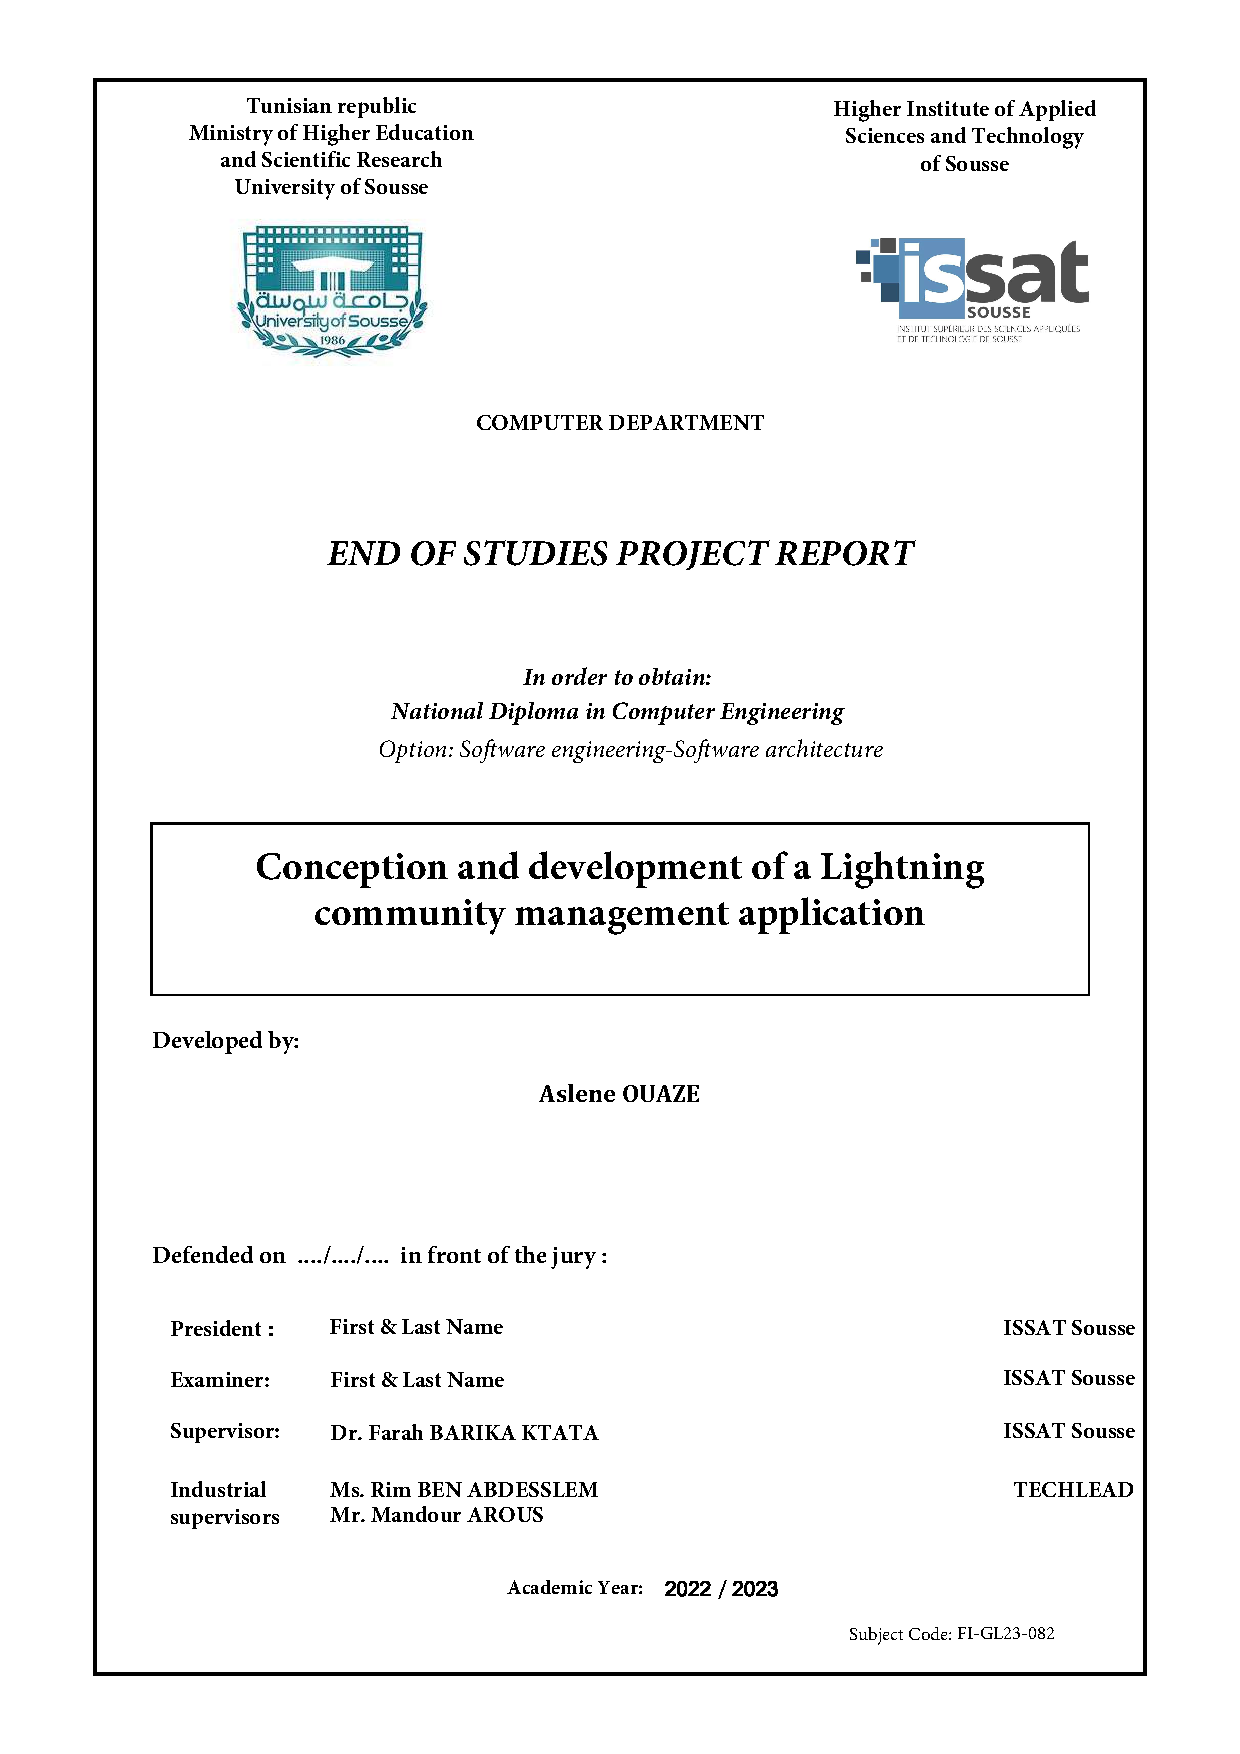
\includepdf[pages=-,fitpaper=true]{page de garde.pdf}
  



    \cleardoublepage%
    % @Author: Jacem Chaieb
% @Date:   2015-07-26 13:42:06
% @Last Modified by:   Jacem Chaieb
% @Last Modified time: 2016-04-12 15:43:36
\chapter*{Thanks}
\addcontentsline{toc}{chapter}{Thanks}
\thispagestyle{empty}
%
At the end of this work, I would like to express my sincere thanks to
all the people who have contributed, directly or indirectly, to its success. ~\\

Lorem ipsum dolor sit amet, consectetur adipisicing elit, sed do eiusmod
tempor incididunt ut labore et dolore magna aliqua. Ut enim ad minim veniam,
quis nostrud exercitation ullamco laboris nisi ut aliquip ex ea commodo
consequat. Duis aute irure dolor in reprehenderit in voluptate velit esse
cillum dolore eu fugiat nulla pariatur. Excepteur sint occaecat cupidatat non
proident, sunt in culpa qui officia deserunt mollit anim id est laborum. Lorem ipsum dolor sit amet, consectetur adipisicing elit, sed do eiusmod
tempor incididunt ut labore et dolore magna aliqua. Ut enim ad minim veniam,
quis nostrud exercitation ullamco laboris nisi ut aliquip ex ea commodo
consequat. Duis aute irure dolor in reprehenderit in voluptate velit esse
cillum dolore eu fugiat nulla pariatur. Excepteur sint occaecat cupidatat non
proident, sunt in culpa qui officia deserunt mollit anim id est laborum.
\chapter*{Dedication}
\addcontentsline{toc}{chapter}{Dedication}
\thispagestyle{empty}
%
%For all they have endured to satisfy all my needs and wishes
\begin{center}
  I dedicate this work to: ~\\
  


  Lorem ipsum dolor sit amet, consectetur adipisicing elit, sed do eiusmod ~\\
  tempor incididunt ut labore et dolore magna aliqua. Ut enim ad minim veniam, ~\\
  quis nostrud exercitation ullamco laboris nisi ut aliquip ex ea commodo ~\\
  consequat. Duis aute irure dolor in reprehenderit in voluptate velit esse ~\\
  cillum dolore eu fugiat nulla pariatur. Excepteur sint occaecat cupidatat non ~\\
  proident, sunt in culpa qui officia deserunt mollit anim id est laborum ~\\
\end{center}
%
\nopagebreak{%
  % And maybe a quote here
  \raggedright\hspace{5.75cm} To all of you,~\\
  \raggedright\hspace{7.75cm} I dedicate this work\@.~\\~\\~\\
  %
  \raggedleft\normalfont\large\itshape{} \reportAuthor\par%
}
%
%
%
%
%
%
\cleardoublepage%

    \cleardoublepage%
% @Author: Jacem Chaieb
% @Date:   2015-07-26 13:42:06
% @Last Modified by:   Jacem Chaieb
% @Last Modified time: 2016-04-12 15:49:40

%%%%%%%%%%%%%%%%%%%%%%%%%%%%
% CHAPTER                  %
%%%%%%%%%%%%%%%%%%%%%%%%%%%%
\thispagestyle{empty}
\vspace*{\fill}
\begingroup
\centering
\begin{center}
{\large \textbf{Résumé}}
\end{center}

Ce travail a été développé dans le cadre d'un projet de stage de fin d'études qui a été réalisé au sein de la
Société TECHLEAD.
Ce projet consiste à concevoir et développer une lightning application dynamique pour le CRM Salesforce
pour permettre aux administrateurs et aux directeurs de communautés de gérer leur communauté et ses utilisateurs.\\
Notre application donne également
la possibilité de consulter l'historique de connexion des utilisateurs et un tableau de bord synthétique visualisant les KPI ainsi que la mise à disposition d'un Chatbot intelligent à l'administrateur.\\~\\
\textbf{Mots clés}\\
Application Lightning, Gestionnaire de communauté, Chatbot, LWC, JS, CSS, Apex, Aura, SLDS, SOQL, SOSL, 
Architecture MVC

\endgroup
\vspace*{\fill}
\cleardoublepage%










\thispagestyle{empty}
\vspace*{\fill}
\begingroup
\centering
\begin{center}
{\large \textbf{Summary}}
\end{center}

This work was developed as part of an end-of-study internship project which was achieved within the
TECHLEAD company.
This project involves designing and developing a dynamic lightning application for the Salesforce CRM
to enable administrators and community managers to manage their community and its users.\\
Our application also gives
the possibility of consulting users' connection history and a synthetic dashboard visualizing the KPIs as well as providing a smart Chatbot to the administrator.\\~\\
\textbf{Keywords}\\
Lightning application, Community Management, Chatbot, LWC, JS, CSS, Apex, Aura, SLDS, SOQL, SOSL, 
MVC Architecture

\endgroup
\vspace*{\fill}





    \cleardoublepage%
    

    \tableofcontents
    %\addcontentsline{toc}{chapter}{\contentsname}
    \cleardoublepage%

    \listoffigures
    %\addcontentsline{toc}{chapter}{\listfigurename}
    \cleardoublepage%

    \listoftables
    %\addcontentsline{toc}{chapter}{\listtablename}
    \cleardoublepage

    %\printglossary[type=\acronymtype, title=Abbreviations]
    

    \sloppy

    \pagenumbering{arabic}% 1 2 3 4 5
    \doublespacing{}% Double spacing between lines

    \addtocontents{toc}{\protect\setcounter{tocdepth}{2}}

    % Main matter
    % @Author: Jacem Chaieb
% @Date:   2015-07-26 13:42:06
% @Last Modified by:   Jacem Chaieb
% @Last Modified time: 2016-04-12 15:49:40

%%%%%%%%%%%%%%%%%%%%%%%%%%%%
% CHAPTER                  %
%%%%%%%%%%%%%%%%%%%%%%%%%%%%
\chapter*{General Introduction}
\addcontentsline{toc}{chapter}{General Introduction}

\markboth{\MakeUppercase{General Introduction}}{}%
In today's digital world, where businesses are increasingly relying on cloud-based services and software,such as the Salesforce Platform, efficient management of user accounts has become crucial. This area demonstrates
multiple important investments thanks to the increasing number of interested developers
in this platform who offer an infinity of useful applications.\\
These applications are accessible everywhere and through multiple devices as long as that device is connected to Salesforce, such availability is provided thanks to the robust web and mobile infrastructure of the Salesforce platform.\\
That's why we wanted to create a lightning solution for individuals and enterprises who want to manage and monitor their user's activity within Salesforce and we took community users as a base point. Our application will provide multiple information and statistics about each user as well as enable modifications to such information, it will also provide useful KPI charts and a smart chatbot solution for administrators and community managers.\\
Our end-of-study project entitled "Salesforce Community Management Lightning Application" concludes our summer training as a computer engineer.\\
The project was carried out over six months, within the company TECHLEAD. This report summarizes the stages of realization of this
project. Its purpose is to situate the context of the project, to describe the resulting application, the methods, and tools used as well as the results obtained.\\
This report follows the following organization:\\
The first chapter is entitled "General Framework of the Project", which is an introductory chapter presenting the host company, the problem, the solution
proposed, and the objectives of the project, a study of the existing and the process of
development of our application.\\
The second chapter, "Specification of needs", is used to identify the actors of our application and then to specify the functional and non-functional needs.
functionalities to which our application must respond, making it possible to identify
its main features.\\
The third chapter, "Conception", serves to describe the conceptual diagrams and the architecture applied to our proposed solution.\\
The fourth and final chapter, "Realization", illustrates the realization
of our project through the presentation of the environment and the development tools as well as the visualization of the results of our work through
the main application interfaces.\\
Finally, we end the report with a general conclusion in which
we recapitulate the work carried out and we present the prospects.


    \cleardoublepage%

    % @Author: Jacem Chaieb
% @Date:   2015-07-26 13:42:06
% @Last Modified by:   Jacem Chaieb
% @Last Modified time: 2016-04-12 15:45:38

%%%%%%%%%%%%%%%%%%%%%%%%%%%%
% CHAPTER                  %
%%%%%%%%%%%%%%%%%%%%%%%%%%%%

\chapter{General framework of the project}%


%%%%%%%%%%%%%%%%%%%%%%%%%%%%
% SECTION                  %
%%%%%%%%%%%%%%%%%%%%%%%%%%%%
\section*{Introduction}
We begin this chapter with a general presentation of the organization
of the reception. We will then detail the context and the problem of our project and
the proposed solution, which will attempt to resolve the inconveniences
that already exist. We will finish this chapter by describing
the schedule of our internship through the Gantt chart as well as the
development process.\\

\section{Presentation of the host organization}
TechLead is a Tunisian IT engineering company whose mission is to design and implement Salesforce solutions for companies to improve their productivity, profitability, and market adaptability.\\
The company supports its clients throughout the life cycle of their projects, from consulting to the complete implementation of the solution and up to the transfer of skills. The company's young, dynamic, and versatile team assists clients in all stages of implementing their Salesforce solution to better interact with customers, partners, and prospects.
The company offers many services such as:
\begin{itemize}
\item[•] \textbf{Accompaniment:} The company's Salesforce advisors help clients implement and develop your Salesforce solution. They can intervene in the audit and analysis of needs, the design, the integration of data, and the configuration of clients' projects quickly and efficiently.
\item[•] \textbf{Support:} The company's experienced developers can provide assistance and maintenance to clients' projects in the various administration or development needs with good availability and responsiveness.
\item[•] \textbf{Salesforce Training:} The company provides training tailored to client's needs and helps them use and leverage the capabilities of Salesforce.
\end{itemize}
\begin{figure}[H]%
    \center   
    
\includegraphics[scale=0.2]{techlead.png}
    \caption{Host organization TECHLEAD}
\end{figure}



\section{Project presentation}
In this part, we put our work in its general context.
first, we present the context. Second, we present the problem and the reasons that led
us to suggest this topic. Third, we present the solution
proposed to solve the problem. Finally, we will describe the objectives
of this project.
\subsection{Context}
Salesforce is a highly customizable advanced CRM, it stores customer data, gives processes to nurture prospective customers, and provides ways to collaborate with other workers. \cite{1} \\
Salesforce comes with a lot of standard functionality, or out-of-the-box products and features that clients can use to run their business. Here are some common things businesses want to do with Salesforce and the features Salesforce gives that support those activities:\cite{1}
\begin{figure}[H]%
    \center   
    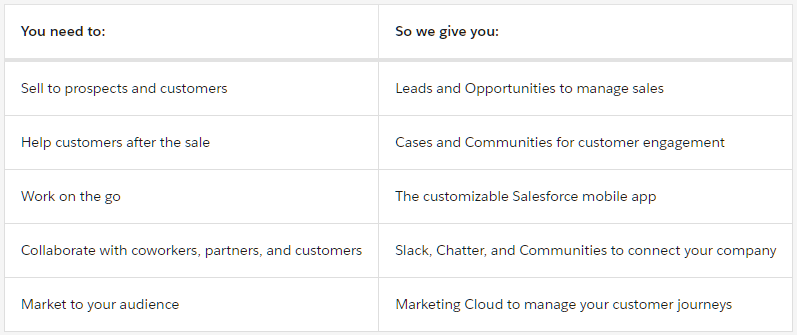
\includegraphics[scale=0.8]{context.png}
    \caption{Salesforce features, Source: \cite{1}}
\end{figure}
The platform also helps clients move fast. Part of that speed comes from replacing tasks that clients are used to doing by hand with more streamlined processes.\cite{2}\\
The platform's goal is to make big changes with minimal effort and to solve mistakes that impact the buyer using dynamic expandable interfaces using additional extensions.
\begin{figure}[H]%
    \center   
    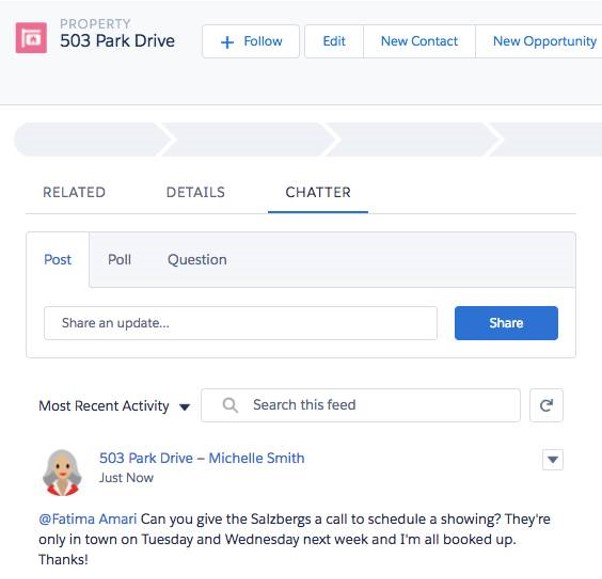
\includegraphics[scale=0.8]{chatter.jpg}
    \caption{Chatter extension in Salesforce, Source: \cite{2}}
\end{figure}
\newpage
Here are a few use cases for different departments:
\begin{figure}[H]%
    \center   
    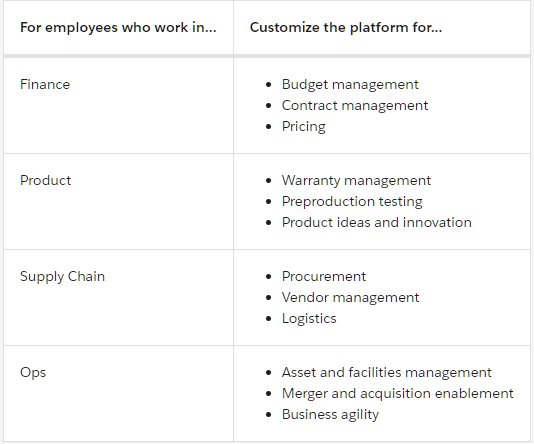
\includegraphics[scale=0.8]{usecases.png}
    \caption{Usecases for Salesforce, Source: \cite{2}}
\end{figure}
Salesforce is a cloud company. Everything to offer resides in the trusted, multitenant cloud.\cite{3} \\
The Salesforce platform is the foundation of the services. It’s powered by metadata and made up of different parts, like data services, artificial intelligence, and robust APIs for development. \cite{3} \\
All the apps sit on top of the platform. The prebuilt offerings like Sales Cloud and Marketing Cloud, along with apps built using the platform, have consistent, powerful functionality.\cite{3} \\
Everything is integrated. The platform technologies like predictive analytics and the development framework are built into everything to offer and everything to build.\cite{3} 
\begin{figure}[H]%
    \center   
    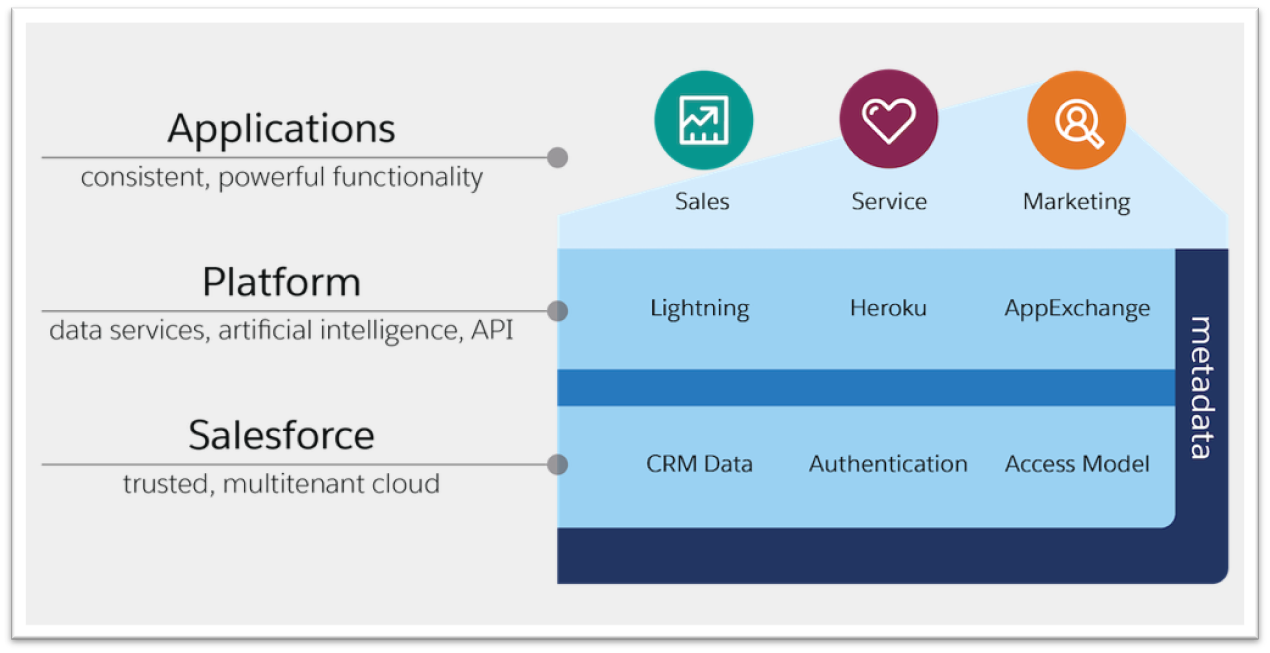
\includegraphics[scale=0.8]{architecture.png}
    \caption{Salesforce's architecture, Source: \cite{3}}
\end{figure}

\subsection{Problem}
In Salesforce, each user is identified by a unique username and profile. Along with other settings, the profile determines what tasks a user can perform, what data they can view, and how they can use the data.\\
As a Salesforce admin, you manage users in your organization. In addition to creating and assigning users, user management includes managing permissions and licenses, delegating users, and more \\

Users are managed in the community through a Salesforce interface and over several stages which makes it difficult and time-consuming.
\subsection{Proposed solution}
The main objective of our work is to design and develop a powerful tool to facilitate the task of managing the users of the community.\\
This application is intended to offer any organization a simple and effective means to manage the "administration" part, then the connection history part, and finally provide a synthetic dashboard visualizing the KPIs as well as a smart Chatbot solution for the administrators and community managers.
\subsection{Objectives}
Ensure user satisfaction by ensuring:\\
\textbf{Functional objectives:}
\begin{enumerate}
\item \textbf{Choice of the community:}
Select the community to which we will manage the users

\item \textbf{Manage users:}
The system must allow users to be managed with the functionalities of activation,
deactivation, modification, and consultation of the list of users via a data table.
Creation of different filters that allow us to facilitate the navigation of the list of users.

\item \textbf{Manage connection history:}
Create a chart that shows the number of user connections per day, week, year, or
according to a well-determined date. This allows the administrator to modify the user’s license

\item \textbf{Offer a synthetic dashboard}
\item \textbf{Offer a smart Chatbot solution}

\end{enumerate}
\textbf{Non-functional objectives:}
\begin{enumerate}
\item\textbf{ Security:} Access to information is only possible after verification of privileges and access rights,
for example Authentication, Redirections.

\item \textbf{Ergonomics and user-friendliness:}
The application will provide a user-friendly and easy-to-use interface that does not
require any prerequisites, so it can be used by all types of users (even non-computer specialists).

\item \textbf{Extensibility and maintainability:}
The architecture of the application will allow the evolution and maintenance (addition
or deletion or update) at the level of its various modules in a flexible manner.

\item \textbf{Performance:}
The application must be efficient, i.e. the system must react within a period that does
not exceed 5 seconds, whatever the action of the application.
\item \textbf{Availability:}
The application will be available on 24/24, and 7/7 except during the maintenance period.

\end{enumerate}
\textbf{Technical objectives:}
\begin{enumerate}
\item Organization of the application according to the MVC architecture: a software architecture model that separates the representation of information from the user's interaction with it.

\begin{figure}[H]%
    \center   
    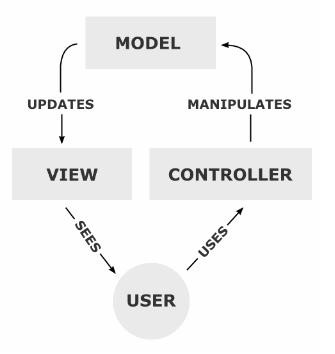
\includegraphics[scale=0.8]{mvc.jpg}
    \caption{MVC Architecture}
\end{figure}

\item Using the Framework "LWC".
\item Using the programming language "Apex".
\item Using the library "SLDS".
\item Using the Salesforce Object Query Language "SOQL/SOSL".

\end{enumerate}
\section{Study of the existing}
In this part, we analyze and criticize the existing applications
currently, through the following table propose a solution that solves
their drawbacks.
\begin{table}[H]
\begin{tabular}{|l|l|l|}
\hline
\textbf{Application} & \textbf{Pros}                                                                                                                                                                                                                                                                                                       & \textbf{Cons}                                                                                                                                                                                                                                                                                                                                                                                           \\ \hline
HubSpot              & \begin{tabular}[c]{@{}l@{}}- User-Friendly Interface\\ - Ability to create custom roles\\ and assign specific permissions\\ to users based on their roles.\\ - Ability tracks user activity,\\ allowing businesses \\ to monitor user behavior.\end{tabular}                                                        & \begin{tabular}[c]{@{}l@{}}- Interface can be complex, \\ particularly for businesses \\ with a large number of users.\\ - Pricing structure is based\\ on the number of contacts\\ in a business's database,\\ which can make it more expensive\\ for businesses with larger teams.\\ - There may be a learning curve\\ when it comes to managing users\\ and configuring access control.\end{tabular} \\ \hline
ZenDesk              & \begin{tabular}[c]{@{}l@{}}- Provides user analytics,\\ allowing businesses \\ to monitor user behavior.\\ - Allows businesses to set up\\ custom notifications for user actions,\\ such as ticket creation or update.\\ - Provides tools for user collaboration,\\ such as shared views and comments.\end{tabular} & \begin{tabular}[c]{@{}l@{}}- May not offer as much granularity\\ as some businesses require.\\ - Interface may not offer \\ as much customization \\ as some businesses require.\\ - Pricing structure is based\\ on the number of agents,\\ which can make it more expensive\\ for businesses with larger teams.\end{tabular}                                                                          \\ \hline
Conga                & \begin{tabular}[c]{@{}l@{}}- Offers customizable workflows.\\ - Offers Centralized \\ user management system.\\ - Provides tools for user collaboration,\\ such as document sharing and commenting\end{tabular}                                                                                                     & \begin{tabular}[c]{@{}l@{}}- Limited third-party integrations\\ - Pricing structure can be\\ more expensive for \\ businesses with larger teams.\\ - User management interface\\ can be complex.\end{tabular}                                                                                                                                                                                           \\ \hline
\end{tabular}
\caption{Study of the existing}
\end{table}
\section{Development process}
A software development process is a set of related activities
followed by a team led to the production of the software within the organization. It consists of a detailed plan describing how to develop, design,
test, deploy, and maintain the product. \cite{4}
\subsection{Incremental development}
In this context, we adopt the process of incremental development as an approach to the realization of our project. According to this process, the customer's needs are specialized, the software is globally designed,
then the realization is done by an increment of functionalities.\cite{4} \\
Each increment
is considered an executable part of the final system. These increments
are successively integrated into the final product and at each stage, the software is
tested, operated, and maintained as a whole.\cite{4} \\
Implementing the software by
increment makes it possible to take into account the risk analysis to facilitate
the detection of errors at the earliest according to customer feedback and to reduce
time and cost of production, which helps in the realization of software
quality. \cite{4}
\subsection{Provisional schedule of tasks}
A Gantt chart is a graphical tool that represents the management
of the project over time, which facilitates its implementation.\\
Indeed, the internship within TECHLEAD will run for a period of 4 months. The following timeline illustrates a provisional schedule set early in development, representing the main stages leading to a functional solution that meets the criteria defined by previusly mentioned specifications.

\begin{figure}[H]%
    \center   
    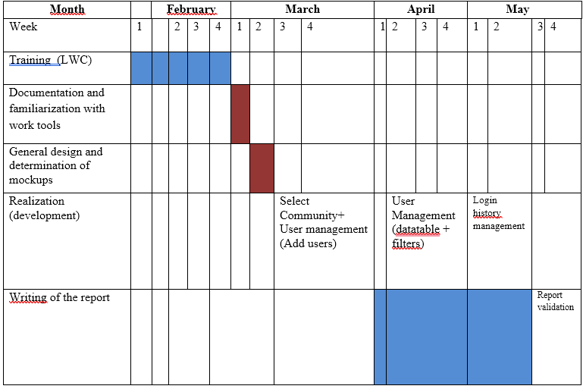
\includegraphics[scale=1]{gantt.png}
    \caption{Gantt diagram}
\end{figure}
\section*{Conclusion}
In this chapter, we have introduced the context of our project by representing the host organization in the first place. Secondly, we have introduced the sales platform and its features. Thirdly, we have
cleared up the problem. Then, we described the proposed solution and
the objectives to be achieved. After that, we analyzed the existing applications. Lastly, we have depicted the advancement of
activities throughout the project according to the adopted development process.
In the next chapter, we will specify the functional requirements and the
non-functional needs.
    \cleardoublepage%
    
    \chapter{Specification of needs}
\section*{Introduction}
In this chapter, we will identify the actors, then we will specify the functional and non-functional needs that the proposed solution must meet. Finally, we present the use case diagrams explaining our application's main functionalities.
\section{Identification of actors}
An actor represents an external entity that interacts directly with the
system. It can be either a human person or a system. We distinguish
two types of actors, the main actor, and a secondary actor. Indeed,
a principal actor obtains an observable result of the system while a
secondary actor is asked for additional information.\\
\subsection*{Main actors}
\textbf{Community Manager}\\
The community manager is the first main user of our application who should be able to :
\begin{itemize}
\item[•] Choose the community that he has the right to access and manage.
\item[•] Consult users of a specific community inside a well-organized table with pagination options.
\item[•] Filter said users by name, user-name, Salesforce account name, status (active or not active), and Salesforce profile.
\item[•] Consult and update the details of each user.
\item[•] Activate users within a specific community.
\item[•] Deactivate users within a specific community.
\item[•] Send a "Welcome to community" email to a specific active user.
\item[•] Send a "Reset password" email to a specific active user.
\item[•] Add one or multiple users at once to a specific community.
\end{itemize}
In case when the community manager has a Salesforce role he will be also able to :
\begin{itemize}
\item[•] Add one or multiple users at once to a specific community.
\end{itemize}
\textbf{Salesforce Administrator}\\
The Salesforce administrator is the second main user of our application who should be able to :
\begin{itemize}
\item[•] Perform all the actions, mentioned above, that the community manager can.
\item[•] Consult a bar chart that shows the number of logins of each user within the selected community.
\item[•] Filter chart results by the period between two specific dates.
\item[•] Consult details about each user displayed in the chart.
\item[•] Update the Salesforce user license for each user displayed in the chart.
\item[•] Consult users failed login attempts to a specific community inside a well-organized table with pagination options.
\item[•] Filter said login attempts by name, user-name, status( Invalid password, No community access, etc... ) and event date and time.
\item[•] Consult detailed information about each login attempt.
\item[•] Send a security warning email to the account owner about the login attempt event.
\item[•] Access a Chatbot that provides information about the selected community or the Salesforce organization.


\end{itemize}
\subsection*{Secondary actors}
\textbf{Salesforce System}\\
This actor is the system, previously developed and deployed in a cloud server by the Salesforce organization, interactable through our application, and it's responsible for :
\begin{itemize}
\item[•] Sending an automatic "Welcome to community" email upon adding a new member to the community by our application user.  
\item[•] Sending an automatic "Welcome to community" email upon activating a previously deactivated user by our application user.
\item[•] Generating reset password URL upon sending a "Reset password" email to a community member by our application user.
\item[•] Tracking users' successful and failed login attempts and saving them to the organization database.

\end{itemize}
\section{Functional Needs}
Functional needs are expressed by the user of the application
which makes it possible to identify the functionalities of this application.\\
In our
case, the functional needs are:
\begin{itemize}
\item Choice of the community:\\
Select the community to which we will manage the users.

\item Manage users:\\
The system must allow users to be managed with the functionalities of activation,
deactivation, modification, and consultation of the list of users via a data table.
Creation of different filters that allow us to facilitate the navigation of the list of users.

\item Manage connection history:\\
Create a chart that shows the number of user connections per day, week, year, or
according to a well-determined date. This allows the administrator to modify the user’s license.


\item Offer a synthetic dashboard:\\
Allowing the system administrator / the community manager to visualize the KPIs (Key Performance Indicators) of his organization/community.


\end{itemize}
\section{Non-functional Needs}
Non-functional requirements represent the characteristics of the system.
They relate to the constraints to be taken into consideration to set up
an adequate solution.\\
For our application, the non-functional requirements are:
\begin{itemize}
\item Security:\\
Access to information is only possible after verification of privileges and access rights,
for example Authentication, Redirections.

\item Ergonomics and user-friendliness:\\
The application will provide a user-friendly and easy-to-use interface that does not
require any prerequisites, so it can be used by all types of users (even non-computer specialists).

\item Extensibility and maintainability:\\
The architecture of the application will allow the evolution and maintenance (addition
or deletion or update) at the level of its various modules in a flexible manner.

\item Performance:\\
The application must be efficient, i.e. the system must react within a period that does
not exceed 5 seconds, whatever the action of the application.

\item Availability:\\
The application will be available on 24/24 and 7/7 except during maintenance.

\end{itemize}
\section{Use case diagrams}
In this section, we will highlight the system's functionalities to be
from the functional needs mentioned above based on the UML(Unified Modeling Language) diagrams which group together all the system's use cases.
\subsection{Global use case diagram}
The following figure illustrates the global use case diagram of our application
\begin{figure}[H]%
    \center   
    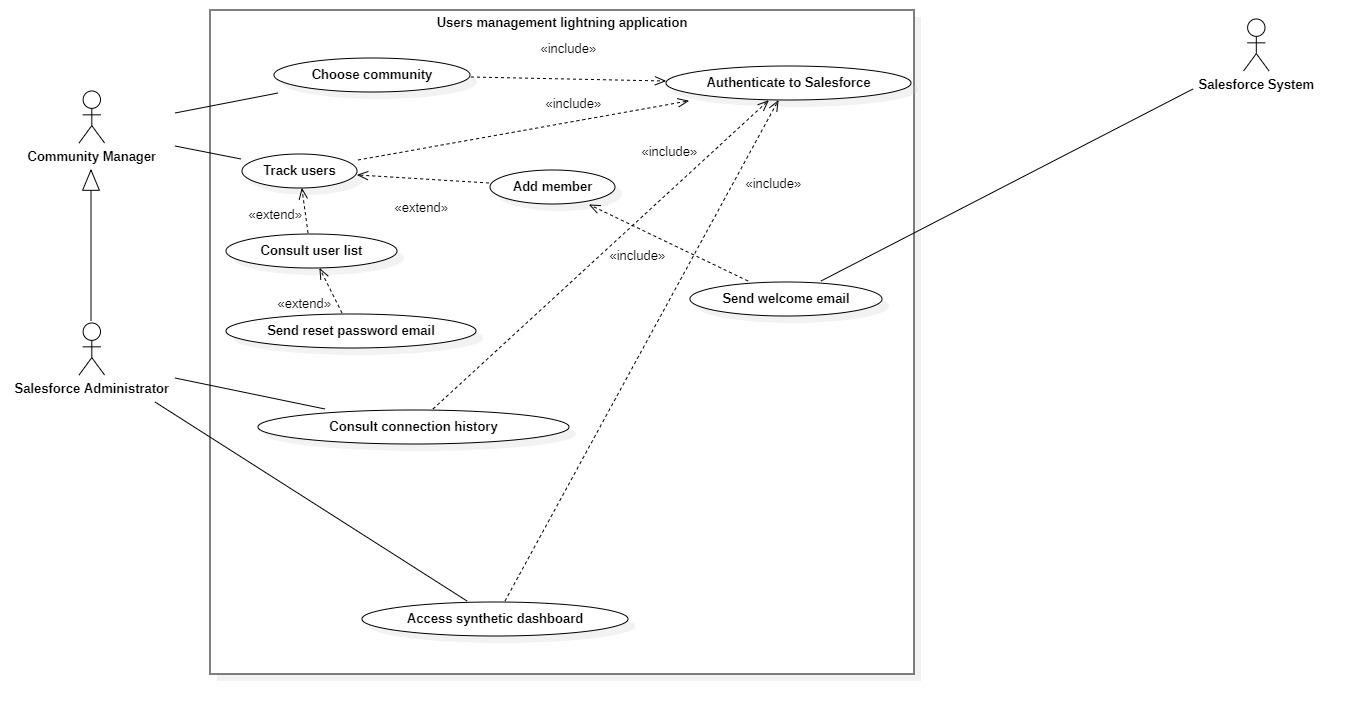
\includegraphics[scale=0.45]{Global UC.jpg}
    \caption{Global use case diagram}
\end{figure}
\subsection{Use case refinement}
In this section, we will detail the main use cases.
\subsubsection{Consult user list use case refinement}
In our application, the community manager and the system administrator can access a data table containing the full list of users within their respective communities.\\
The following figure shows the Consult user list use case diagram.
\begin{figure}[H]%
    \center   
    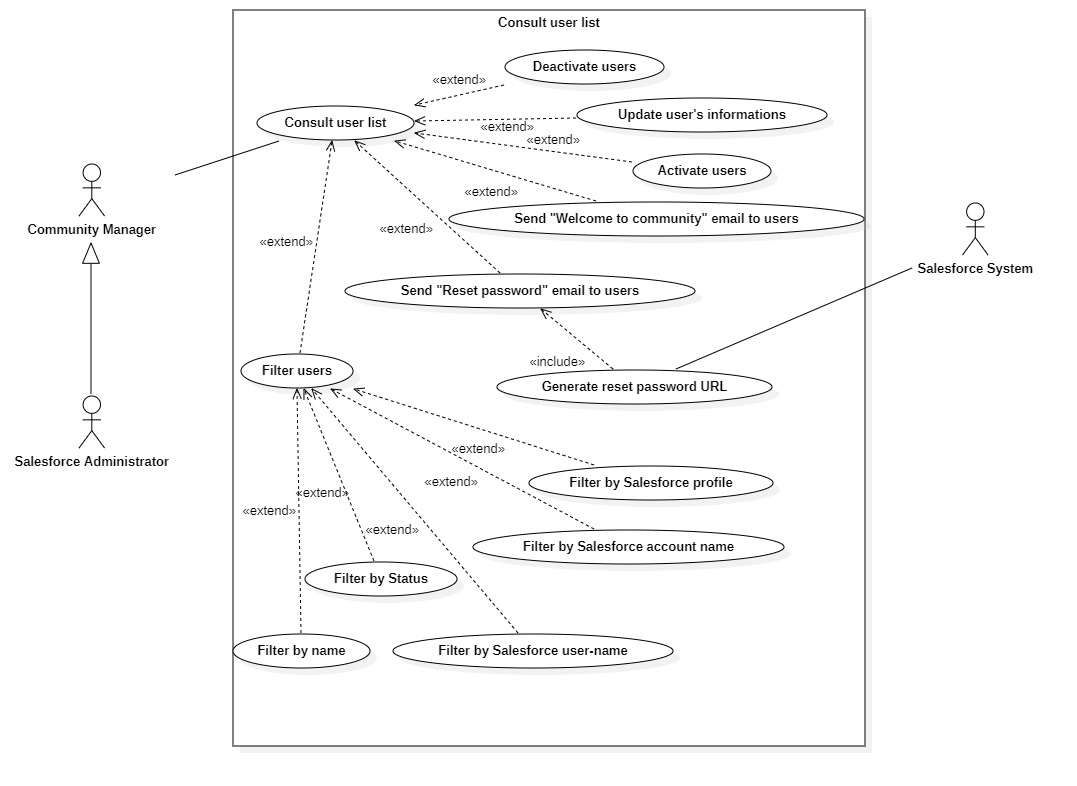
\includegraphics[scale=0.5]{Consult users list UC.jpg}
    \caption{Consult user list use case diagram}
\end{figure}
The following table details the tasks to be performed by the user to manage the user list.

\begin{table}[H]
\footnotesize% or \small or \scriptsize
\begin{tabular}{|ll|}
\hline
\multicolumn{2}{|c|}{\textbf{Summary}}                                                                                                                                                                                                                                                                                                                                                                                                                                                                                                                                                                                                                                                                                                                                                         \\ \hline
\multicolumn{1}{|l|}{Title}                      & Consult user list                                                                                                                                                                                                                                                                                                                                                                                                                                                                                                                                                                                                                                                                                                                           \\ \hline
\multicolumn{1}{|l|}{Objectif}                   & \begin{tabular}[c]{@{}l@{}}Allowing the community manager or the system administrator\\ to manage his community members\end{tabular}                                                                                                                                                                                                                                                                                                                                                                                                                                                                                                                                                                                                        \\ \hline
\multicolumn{1}{|l|}{Actors}                     & Community manager, System administrator                                                                                                                                                                                                                                                                                                                                                                                                                                                                                                                                                                                                                                                                                                     \\ \hline
\multicolumn{2}{|c|}{\textbf{Description of sequences}}                                                                                                                                                                                                                                                                                                                                                                                                                                                                                                                                                                                                                                                                                                                                        \\ \hline
\multicolumn{1}{|l|}{Pre-condition}              & \begin{tabular}[c]{@{}l@{}}- User should be authenticated to Salesforce\\ - User should be the owner of at least one community\end{tabular}                                                                                                                                                                                                                                                                                                                                                                                                                                                                                                                                                                                                 \\ \hline
\multicolumn{1}{|l|}{Post-condition}             & - Community members are well organized                                                                                                                                                                                                                                                                                                                                                                                                                                                                                                                                                                                                                                                                                                      \\ \hline
\multicolumn{1}{|l|}{Normal scenario}            & \begin{tabular}[c]{@{}l@{}}1. User accesses the user list interface\\ 2. User selects one or many community members\\ 3. User clicks the "activate/deactivate" button for selected members\\ 4. The system prompts the success of the operation\\ 5. The user clicks the "Send welcome email" button\\ for the selected members\\ 6. The system prompts the success of the operation\\ 7. The user clicks the "Send reset password" button\\ for the selected members\\ 8. The system prompts the success of the operation\\ 9. The user clicks the "show details" button for one member\\ 10. The member information interface pops up \\ 11. User updates the selected member information and complies\\ 12. System prompts the success of the operation\end{tabular} \\ \hline
\multicolumn{1}{|l|}{Alternative scenario}       & \begin{tabular}[c]{@{}l@{}}1. License limit exceeded when activating members: The system\\ sends an error message\\ 2. Sending a welcome email to a deactivated member: The system\\ sends an error message\\ 3. Changing member username to an existing one: The system\\ sends an error message\end{tabular}                                                                                                                                                                                                                                                                                                                                                                                                                              \\ \hline
\multicolumn{1}{|l|}{Non-functional constraints} & \begin{tabular}[c]{@{}l@{}}1. The interface must be ergonomic\\ 2. Error messages should be understandable and clear\end{tabular}                                                                                                                                                                                                                                                                                                                                                                                                                                                                                                                                                                                                           \\ \hline
\end{tabular}
\captionsetup{skip=5pt} % Adjust the skip value as per your needs
\caption{Consult user list use case}

\end{table}
\pagebreak
\subsubsection{Add members use case refinement}
In our application, the community manager and the system administrator can add one or multiple members at once to their respective communities.\\

The following table details the tasks to be performed by the user to add members to his community.

\begin{table}[H]
\begin{tabular}{|ll|}
\hline
\multicolumn{2}{|c|}{\textbf{Summary}}                                                                                                                                                                                                                                                                                                                                                                                                                                                                                                                                                                                                                                                                                      \\ \hline
\multicolumn{1}{|l|}{Title}                      & Add members                                                                                                                                                                                                                                                                                                                                                                                                                                                                                                                                                                                                                                                              \\ \hline
\multicolumn{1}{|l|}{Objectif}                   & \begin{tabular}[c]{@{}l@{}}Allowing the community manager or the system administrator to \\ add one or multiple members at once to his community\end{tabular}                                                                                                                                                                                                                                                                                                                                                                                                                                                                                                            \\ \hline
\multicolumn{1}{|l|}{Actors}                     & Community manager, System administrator                                                                                                                                                                                                                                                                                                                                                                                                                                                                                                                                                                                                                                  \\ \hline
\multicolumn{2}{|c|}{\textbf{Description of sequences}}                                                                                                                                                                                                                                                                                                                                                                                                                                                                                                                                                                                                                                                                     \\ \hline
\multicolumn{1}{|l|}{Pre-condition}              & \begin{tabular}[c]{@{}l@{}}- User should be authenticated to Salesforce\\ - User should be the owner of at least one community\\ - User should have a Salesforce role\end{tabular}                                                                                                                                                                                                                                                                                                                                                                                                                                                                                       \\ \hline
\multicolumn{1}{|l|}{Post-condition}             & - New member(s) are added to the owner's community                                                                                                                                                                                                                                                                                                                                                                                                                                                                                                                                                                                                                       \\ \hline
\multicolumn{1}{|l|}{Normal scenario}            & \begin{tabular}[c]{@{}l@{}}1. User accesses the add members interface\\ 2. The user fills the displayed form with information about the new member\\ 3. The user clicks the " add another member" button\\ 4. A new empty form, identical to the previous one, is displayed\\ 5. The user fills the new form with information about the next new member\\ 6. The user clicks the "clone member" button\\ 7. A new form containing the same values as the previous form is displayed\\ 8. The user clicks the "delete form" button\\ 9. The selected form is deleted from the screen\\ 10. The user clicks the "submit" button \\ 11. System prompts the success of the operations\end{tabular} \\ \hline
\multicolumn{1}{|l|}{Alternative scenario}       & \begin{tabular}[c]{@{}l@{}}1. Empty fields: The system sends an error message:\\ You must complete all the required fields\\ 2. The email entered is not valid: The system sends an error message\\ describing the validation conditions for this field\\ 3. Duplicate Salesforce user-name: The system sends an error message\end{tabular}                                                                                                                                                                                                                                                                                                                              \\ \hline
\multicolumn{1}{|l|}{Non-functional constraints} & \begin{tabular}[c]{@{}l@{}}1. The interface must be ergonomic\\ 2. Error messages should be understandable and clear\end{tabular}                                                                                                                                                                                                                                                                                                                                                                                                                                                                                                                                        \\ \hline
\end{tabular}
\captionsetup{skip=5pt} % Adjust the skip value as per your needs
\caption{Add members use case}

\end{table}
\subsubsection{Consult synthetic dashboard use case refinement}
In our application, the community manager and the system administrator can access a dashboard containing features that helps them to manage their respective communities.\\
The following figure shows the Consult synthetic use case diagram.
\begin{figure}[H]%
    \center   
    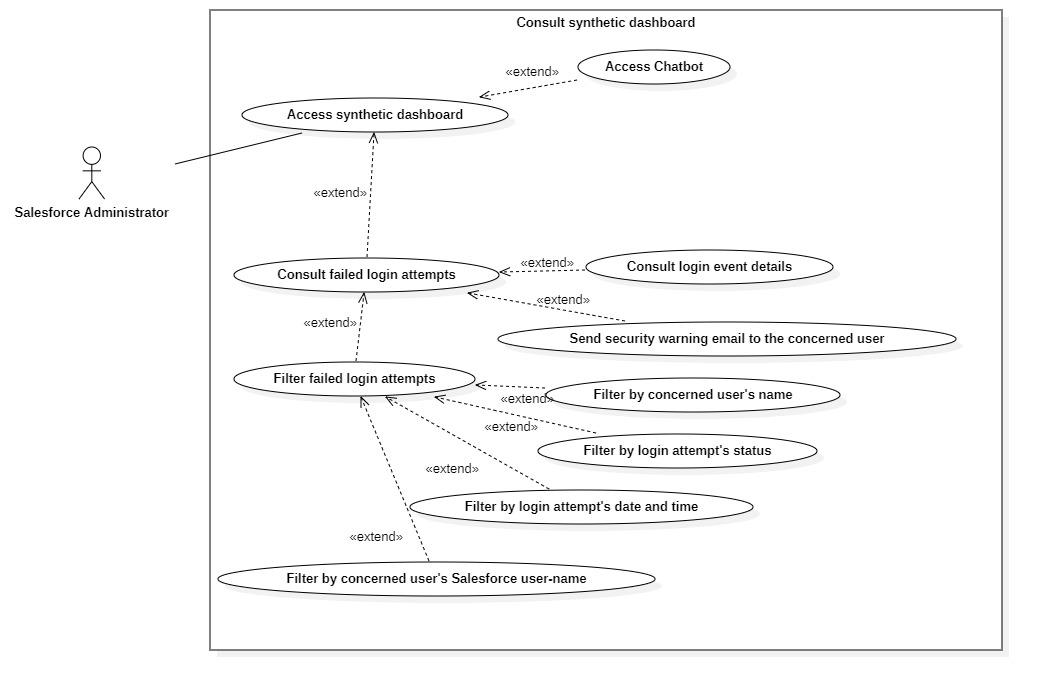
\includegraphics[scale=0.5]{Consult synthetic dashboard UC.jpg}
    \caption{Consult synthetic dashboard use case diagram}
\end{figure}

The following table details the tasks to be performed by the customer to consult the synthetic dashboard
in our application.
\begin{table}[H]
\begin{tabular}{|ll|}
\hline
\multicolumn{2}{|c|}{\textbf{Summary}}                                                                                                                                                                                       \\ \hline
\multicolumn{1}{|l|}{Title}                      & Consult synthetic dashboard                                                                                                                                               \\ \hline
\multicolumn{1}{|l|}{Objectif}                   & \begin{tabular}[c]{@{}l@{}}Allowing the system administrator\\ to access extra features that helps him to manage his communities\end{tabular} \\ \hline
\multicolumn{1}{|l|}{Actors}                     & System administrator                                                                                                                                   \\ \hline
\multicolumn{2}{|c|}{\textbf{Description of sequences}}                                                                                                                                                                      \\ \hline
\multicolumn{1}{|l|}{Pre-condition}              & \begin{tabular}[c]{@{}l@{}}- User should be authenticated to Salesforce\\ - User should be the owner of at least one community\end{tabular}                               \\ \hline
\multicolumn{1}{|l|}{Post-condition}             & \begin{tabular}[c]{@{}l@{}}- System administrator is well informed\\ about his respective community.\end{tabular}                                \\ \hline
\multicolumn{1}{|l|}{Normal scenario}            & \begin{tabular}[c]{@{}l@{}}1. User accesses the dashboard interface\\ 2. User selects the wanted feature \\ 3. The selected feature interface pops up.\end{tabular}       \\ \hline
\multicolumn{1}{|l|}{Alternative scenario}       &                                                                                                                                                                           \\ \hline
\multicolumn{1}{|l|}{Non-functional constraints} & 1. The interface must be ergonomic                                                                                                                                        \\ \hline
\end{tabular}
\caption{Consult synthetic dashboard use case}
\end{table}


The following table details the tasks to be performed by the customer to consult the failed login attempts
in our application.
\begin{table}[H]
\begin{tabular}{|ll|}
\hline
\multicolumn{2}{|c|}{\textbf{Summary}}                                                                                                                                                                                                                                                                                                                                                                                                                                                                                                                           \\ \hline
\multicolumn{1}{|l|}{Title}                      & Consult failed login attempts                                                                                                                                                                                                                                                                                                                                                                                                                                                                                 \\ \hline
\multicolumn{1}{|l|}{Objectif}                   & \begin{tabular}[c]{@{}l@{}}Allowing  the system administrator\\ to access failed login attempts and inform concerned users about them\end{tabular}                                                                                                                                                                                                                                                                                                                                                            \\ \hline
\multicolumn{1}{|l|}{Actors}                     & System administrator                                                                                                                                                                                                                                                                                                                                                                                                                                                                                          \\ \hline
\multicolumn{2}{|c|}{\textbf{Description of sequences}}                                                                                                                                                                                                                                                                                                                                                                                                                                                                                                          \\ \hline
\multicolumn{1}{|l|}{Pre-condition}              & \begin{tabular}[c]{@{}l@{}}- User should be authenticated to Salesforce\\ - User should be the owner of at least one community\end{tabular}                                                                                                                                                                                                                                                                                                                                                                   \\ \hline
\multicolumn{1}{|l|}{Post-condition}             & - Users are well-informed about their account security status.                                                                                                                                                                                                                                                                                                                                                                                                                                                \\ \hline
\multicolumn{1}{|l|}{Normal scenario}            & \begin{tabular}[c]{@{}l@{}}1. User accesses the failed login attempts interface\\ 2. The user clicks the "show details" button for a specific login event\\ 3. The "show details" interface for the selected login event pops up\\ 4. The user clicks the "send security warning email" button for\\ the specific login event\\ 5. The system prompts the success of the operation\\ 6. The concerned user receives the warning email, containing details\\ about the failed login attempt, in his email\end{tabular} \\ \hline
\multicolumn{1}{|l|}{Alternative scenario}       & \begin{tabular}[c]{@{}l@{}}1. Server error when sending the warning email: The system\\ sends an error message received from the server\end{tabular}                                                                                                                                                                                                                                                                                                                                                          \\ \hline
\multicolumn{1}{|l|}{Non-functional constraints} & \begin{tabular}[c]{@{}l@{}}1. The interface must be ergonomic\\ 2. Error messages should be understandable and clear\end{tabular}                                                                                                                                                                                                                                                                                                                                                                             \\ \hline
\end{tabular}
\caption{Consult failed login attempts use case}
\end{table}



\subsubsection{Access Chatbot use case refinement}
The following figure illustrates the use case diagram "Access Chatbot"

\begin{figure}[H]%
    \center   
    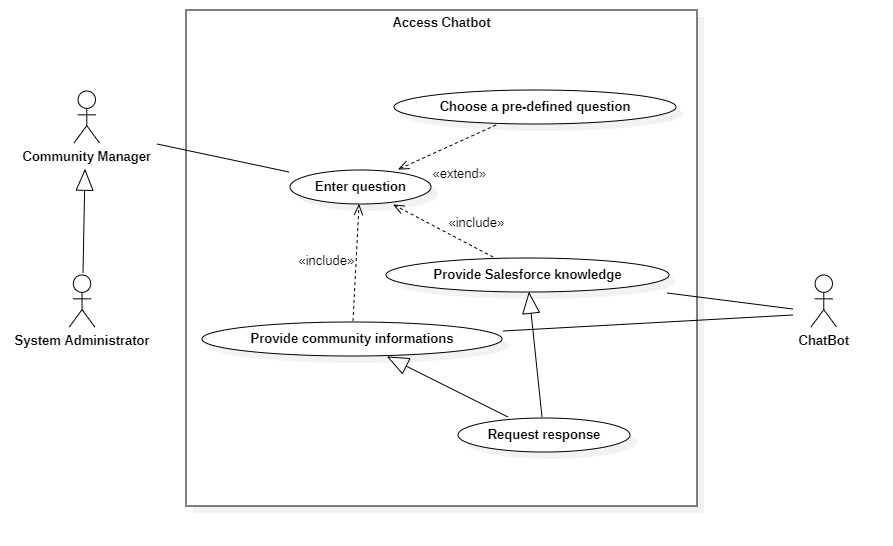
\includegraphics[scale=0.5]{Access Chatbot.jpg}
    \caption{Access Chatbot use case diagram}
\end{figure}

The following table details the tasks to be performed by the customer to Access the Chatbot within our app.
\begin{table}[H]
\begin{tabular}{|ll|}
\hline
\multicolumn{2}{|c|}{\textbf{Summary}}                                                                                                                                                                                                                                                                                                                              \\ \hline
\multicolumn{1}{|l|}{Title}                      & Access Chatbot                                                                                                                                                                                                                                                                                                   \\ \hline
\multicolumn{1}{|l|}{Objectif}                   & \begin{tabular}[c]{@{}l@{}}Trigger a Chatbot that responds to user requests \\ while providing informations about the current community\end{tabular}                                                                                                                                                             \\ \hline
\multicolumn{1}{|l|}{Actors}                     & System administrator, Chatbot                                                                                                                                                                                                                                                                                    \\ \hline
\multicolumn{2}{|c|}{\textbf{Description of sequences}}                                                                                                                                                                                                                                                                                                             \\ \hline
\multicolumn{1}{|l|}{Pre-condition}              & \begin{tabular}[c]{@{}l@{}}- User should be authenticated to Salesforce\\ - User should be the owner of at least one community\end{tabular}                                                                                                                                                                      \\ \hline
\multicolumn{1}{|l|}{Post-condition}             & \begin{tabular}[c]{@{}l@{}} - User question is answered\\ and the response is displayed on the screen. \end{tabular}                                                                                                                                                                                                                                             \\ \hline
\multicolumn{1}{|l|}{Normal scenario}            & \begin{tabular}[c]{@{}l@{}}1. User accesses the Chatbot interface\\ 2. User types a question or selects a predefined question.\\ 3. The chatbot is launched upon receipt of a request\\ 4. The chatbot analyzes the request\\5. The chatbot prepares the response\\ 6. The chatbot sends the response\end{tabular} \\ \hline
\multicolumn{1}{|l|}{Alternative scenario}       & 1. An error message is displayed if the question\\ is not recognized by the system.                                                                                                                                                                                                                                 \\ \hline
\multicolumn{1}{|l|}{Non-functional constraints} & \begin{tabular}[c]{@{}l@{}}1. The interface must be ergonomic\\ 2. Error messages should be understandable and clear\\ 3. The ChatBot must always be available.\end{tabular}                                                                                                                                     \\ \hline
\end{tabular}

\caption{Access Chatbot use case}
\end{table}

\pagebreak
\section*{Conclusion}
In this chapter, we have described the specification phases of the
needs of our developed application to identify the different actors
as well as the features and services that our application must provide.\\
We have detailed these features with use case diagrams. The next chapter will be devoted to the conception phase.
    \cleardoublepage%
    \chapter{Conception}
\section*{Introduction}
After identifying the functional and non-functional needs and the main functionalities of our application. We begin this part
of the conceptual study by describing the general architecture of our system and
it's detailed internal modeling through class and sequence diagrams.
\section{Global Architecture}
In this section, we will give an overview of the definition of the
the architectural pattern was chosen to model our application and we will
detail the projection of this pattern on our application.

\subsection{Definition of the Model-View-Controller design pattern}
Our chosen architecture of work for this project will be the MVC  architecture since it is recommended by the Salesforce developer’s community.\\
The model-view-controller (MVC) design pattern specifies that an application consists of a data model, presentation information, and control information.\cite{5} \\
The pattern requires that each of these be separated into different objects:
\begin{itemize}
\item \textbf{The model} (for example, the data information) contains only pure application data; it contains no logic describing how to present the data to a user. \cite{5}
\item \textbf{The view} (for example, the presentation information) presents the model's data to the user. The view knows how to access the model's data but does not know what this data means or what the user can do to manipulate it. \cite{5}
\item \textbf{The controller} (for example, the control information) exists between the view and the model. It listens to events triggered by the view (or another external source) and executes the appropriate reaction to these events. In most cases, the reaction is to call a method on the model. Since the view and the model are connected through a notification mechanism, the result of this action is then automatically reflected in the view.\cite{5}
\end{itemize}
Thanks to these principles, the components of the application become easy to
manage, test, modify, and reuse.\\
The following figure explains furthermore the role and the idea behind each component of the MVC pattern:

\begin{figure}[H]%
    \center   
    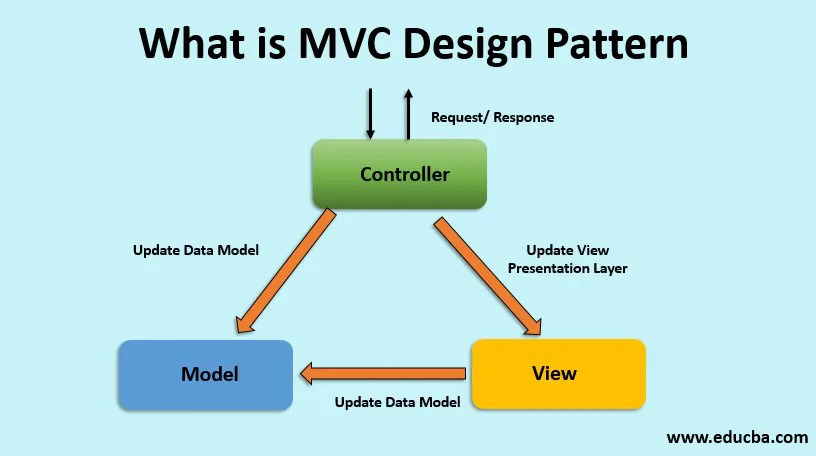
\includegraphics[scale=0.5]{mvc2.jpg}
    \caption{Understanding MVC Design Pattern, Source: \cite{7}}
\end{figure}
\subsection{Application of the "MVC" pattern}
We explain in this paragraph the details of the projection of the pattern
MVC on our app.\\
The following figure represents the class diagram which illustrates the binding
between entities (classes). Indeed, this diagram translates the content of the \textbf{Model} component, and it's based on the schema that is already established within the Salesforce infrastructure.
\begin{figure}[H]%
    \center   
    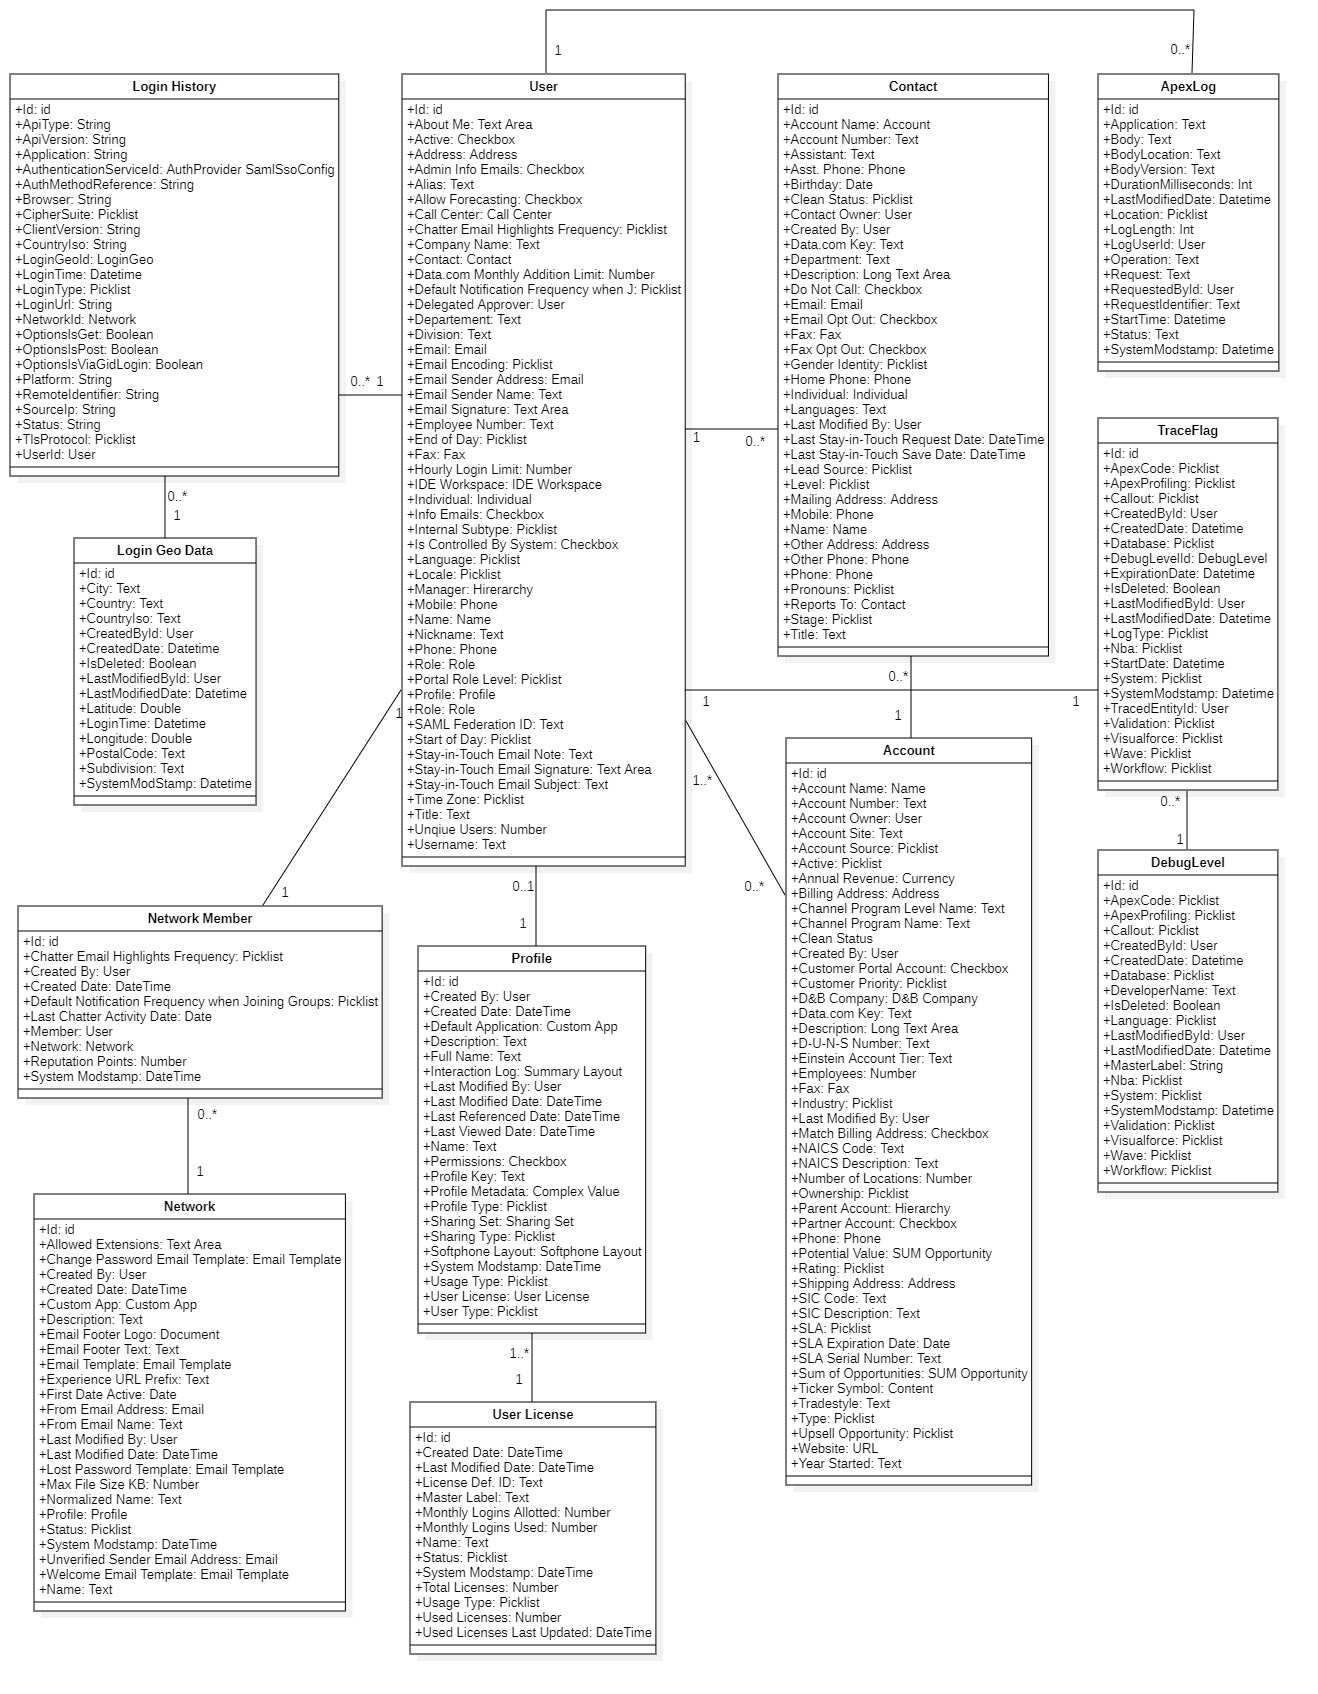
\includegraphics[scale=0.4]{ClassDiagram.jpg}
    \caption{Class diagram representing the "Model" component}
\end{figure}
\newpage
Description of classes representing our Model:
\begin{itemize}
\item \textbf{User:}\\
This class represents our application's Salesforce user, who is the main focus of the administrator and community managers main focus when working within our app. This class's most important attributes in our application are:
\begin{itemize}
\item[•] Id: the unique identification key for the user 
\item[•] Active: determines the status of the user (active or not active)
\item[•] Address: the full address of the user
\item[•] Alias: the alias of the user, usually composed of the first letter of his first name and his last name concatenated together
\item[•] Contact: a lookup field that connects the user to its corresponding Salesforce contact which is necessary to have to allow the user to access a community
\item[•] Email: the email of the user
\item[•] Email Encoding: the encoding of the user's email (for example UTF-8), useful for sending appropriate emails to the user
%\item[•] First Name: the first name of the user
\item[•] Is Portal Enabled: determines if the user can access a community or not
%\item[•] Last Name: the last name of the user
\item[•] Language: the preferred interface language of the user that will control the user interface of the accessed community
\item[•] Locale: the geolocation locale id of the user ( example Arabic(Tunisia) )
\item[•] Name: the full name of the user which is composed automatically by the Salesforce system by concatenating his first name and his last name
\item[•] Profile: a lookup field that connects the user to its corresponding Salesforce profile which controls the level of access provided to the user ( for example System Administrator which gives full access to all Salesforce objects and configurations )
\item[•] Role: the relative company role of the user ( for example CEO ), this field is required to be able to add a user to a community through our app
\item[•] Time Zone: the timezone of the user ( for example GMT+02:00 )
\item[•] Username: the unique Salesforce user name if the user usually identical to the user's email
\end{itemize}
\item \textbf{Contact:}\\
This class represents the Salesforce contacts connected to the community user in our application. This class's most important attributes in our application are:
\begin{itemize}
\item[•] Id: the unique identification key for the contact 
\item[•] Account Name: a lookup field that represents the Salesforce unique account connected to the contact
\item[•] Contact Owner: a lookup field that represents the user owning the Salesforce contact
\item[•] Created By:: a lookup field that represents the user who created the Salesforce contact
\item[•] Email: email of the contact
\item[•] Last Modified By: a lookup field that represents the last user to modify details of the contact
\item[•] Name: the full name of the contact

\end{itemize}
\item \textbf{Account}\\
This class represents the Salesforce account connected to the community user in our application. This class's most important attributes in our application are:
\begin{itemize}
\item[•] Id: the unique identification key for the account 
\item[•] Account Name: Salesforce account name
\item[•] Account Owner: a lookup field that represents the user owning the Salesforce account 
\item[•] Created By: a lookup field that represents the user who created the Salesforce account 
\item[•] Customer Portal Account: determines if the account can be connected to the community user
\item[•] Last Modified By: a lookup field that represents the last user to modify details of the account
\item[•] Parent Account: a self-lookup field that represents the parent account of this account through the Salesforce hierarchy
\end{itemize}
\item \textbf{Profile}\\
This class represents the Salesforce profile connected to the community user in our application. This class's most important attributes in our application are:
\begin{itemize}
\item[•] Id: the unique identification key for the profile 
\item[•] Created By: a lookup field that represents the user who created the Salesforce profile 
\item[•] Full Name: the full name of the profile that represents its usage context 
\item[•] Last Modified By: a lookup field that represents the last user to modify details of the profile
\item[•] Name: the name of the Salesforce profile that represents the main way of identifying the profile through other objects
\item[•] User License: a lookup field that represents the Salesforce purchased user license connected to the profile 

\end{itemize}
\item \textbf{User License}\\
This class represents the Salesforce purchased user license connected to the community user in our application. This class's most important attributes in our application are:
\begin{itemize}
\item[•] Id: the unique identification key for the user license 
\item[•] Name: the name of the Salesforce user license that represents the main way of identifying the user license through other objects
\item[•] Total Licenses: represents the total number of purchased user licenses dedicated to community users 
\item[•] Used Licenses: represents the number of used user licenses which determines if the administrator or the community manager can add more users to his community depending on how many purchased user licenses are left

\end{itemize}
\item \textbf{Network}\\
This class represents the community created by our application's administrator or the community manager. This class's most important attributes in our application are:
\begin{itemize}
\item[•] Id: the unique identification key for the network 
\item[•] Created By: a lookup field that represents the user who created the Salesforce community 
\item[•] Created Date: represents the date and time of the creation of the Salesforce community
\item[•] Description: a brief description of the community set by its creator to summarize its purpose
\item[•] From Email Address: represents the email that will be displayed when a user receives an email through our application
\item[•] From Email Name: represents the name that will be displayed when a user receives an email through our application
\item[•] Last Modified By: a lookup field that represents the last user to modify details or the content of the community
\item[•] Last Modified Date: represents the date and time of the last activity within the community
\item[•] Lost Password Template: represents the email template that will be used when sending a "Reset password" email through our application
\item[•] Name: the name of the Salesforce community that represents the main way of identifying the community through other objects
\item[•] Profile: a lookup field that represents the Salesforce profiles that are allowed to access the community
\item[•] Welcome Email Template: represents the email template that will be used when sending a "Welcome to community" email through our application
\end{itemize}
\item \textbf{Network Member}\\
This class represents the users that are considered members of a Salesforce community in our application. This class's most important attributes in our application are:
\begin{itemize}
\item[•] Id: the unique identification key for the network member
\item[•] Created By: a lookup field that represents the user who added the new member to the Salesforce community 
\item[•] Member: a lookup field that represents the user representing the member of the community, this field is used to access all the details about the user within the Network Member object
\item[•] Network: a lookup field that represents the community that the member is considered a part of, this field is used to access all the details about the community within the Network Member object


\end{itemize}

\item \textbf{Login History}\\
This class represents the login event details that are recorded by Salesforce regarding users' activity and will be used to track the activities of the members of any Salesforce community in our application. This class's most important attributes in our application are:
\begin{itemize}
\item[•] Id: the unique identification key for the login history
\item[•] Browser: represents the commercial name and the version of the web browser that the login vent happened from ( for example Chrome 112 ) 
\item[•] CountryIso: the first two letters of the country where the login event happened from ( for example TN stands for Tunisia )
\item[•] LoginGeoId: a lookup field that represents the geographic location connected to the login event
\item[•] LoginTime: the exact date and time of the login event
\item[•] NetworkId:  a lookup field that represents the community that the user wanted to access when the login event was recorded
\item[•] Platform: represents the commercial name and the version of the platform that the login vent happened from ( for example Windows 10 )
\item[•] SourceIp: the IP address of the user that tried to access the community 
\item[•] Status: the state of the login attempt ( for example Invalid Password )
\item[•] UserId: a lookup field that represents the user concerned with the login event, this field is used to send security warning emails, within our application, to users concerned with a failed login attempt 

\end{itemize}
\item \textbf{LoginGeo}\\
This class represents the login event's geographic location details that are recorded by Salesforce regarding users' activity and will be used to track the geographic location of the activities of the members of any Salesforce community in our application. This class's most important attributes in our application are:
\begin{itemize}
\item[•] Id: the unique identification key for the loginGeo
\item[•] City: represents the city when the login event happened (for example Mahdia)
\item[•] Country: represents the country when the login event happened (for example Tunisia)
\item[•] CountryIso: the first two letters of the country where the login event happened from ( for example TN stands for Tunisia )
\item[•] Latitude: represents the geographic latitude of the login event
\item[•] Longitude: represents the geographic longitude of the login event

\end{itemize}
\item \textbf{TraceFlag}\\
This class represents the tracked users and entities regarding monitoring logs for programming errors and bugs committed by developers in the community and will be used to register said users so that their error logs will be monitored by the administrator. This class's most important attributes in our application are:
\begin{itemize}
\item[•] Id: the unique identification key for the traceFlag
\item[•] StartDate: represents the tracking event's starting date for the created trace flag
\item[•] ExpirationDate: represents the expiration date for the created trace flag
\item[•] DebugLevelId: a lookup field that connects the traceflag to the Debulevel object in Salesforce, in our application this field will have the default value of the SFDC DevConsole's Id 
\item[•] LogType: determines the type of logging that will be returned when requesting it, in our application, it will take the default value of "USER \_ DEBUG" since we will be tracking users' error logs
\item[•] TracedEntityId: represents the id of the tracked user

\end{itemize}
\item \textbf{DebugLevel}\\
This class represents a configuration setting that determines the level of detail for debugging and logging activities in the system. This class's most important attributes in our application are:
\begin{itemize}
\item[•] Id: the unique identification key for the debugLevel
\item[•] MasterLabel: represents debugLevel main label that will be used in our application to retrieve the id of the object and connect it to the TraceFlag object

\end{itemize}
\item \textbf{ApexLog}\\
This class represents the detailed logs of the execution of all Apex code run by the tracked user within the community, and it will be used in our application to provide said logs to the administrator. This class's most important attributes in our application are:
\begin{itemize}
\item[•] Id: the unique identification key for the apexLog
\item[•] Body: represents the plain text containing execution traces, debug operations and outputs, and errors provided by the called Apex methods
\item[•] LogUserId: a lookup field representing the user who ran the Apex code which generated the ApexLog
\item[•] StartDate: represents the date and time marking the beginning of the Apex code's execution
\item[•] Status: represents the title of the main event's log (for example out of bound exception)

\end{itemize}
\end{itemize}
%End of page 35 in the Selma report%
The classes we have defined in the "Model" component are related to the Salesforce object infrastructure, and employable in various types of features in our application. Thus, we made the
principle of independence between the business rules and the application rules.\\


\section{Dynamic view of the application}
In this section, we will describe the internal dynamic of our application using sequence diagrams 
\subsection{Detailed sequence diagram of the "Choose community" use case}
The following figure illustrates the detailed sequence diagram of the use case
"Choose community".
This use case starts with opening a community list interface
for the user. Then, the user may enter his searched community name or a few letters of it.
The system displays an error message if there are no communities found with the entered name otherwise it displays found communities. Then the user may choose to access one of the displayed communities, then the system redirects the user to that community dashboard. 
\begin{figure}[H]%
    \center   
    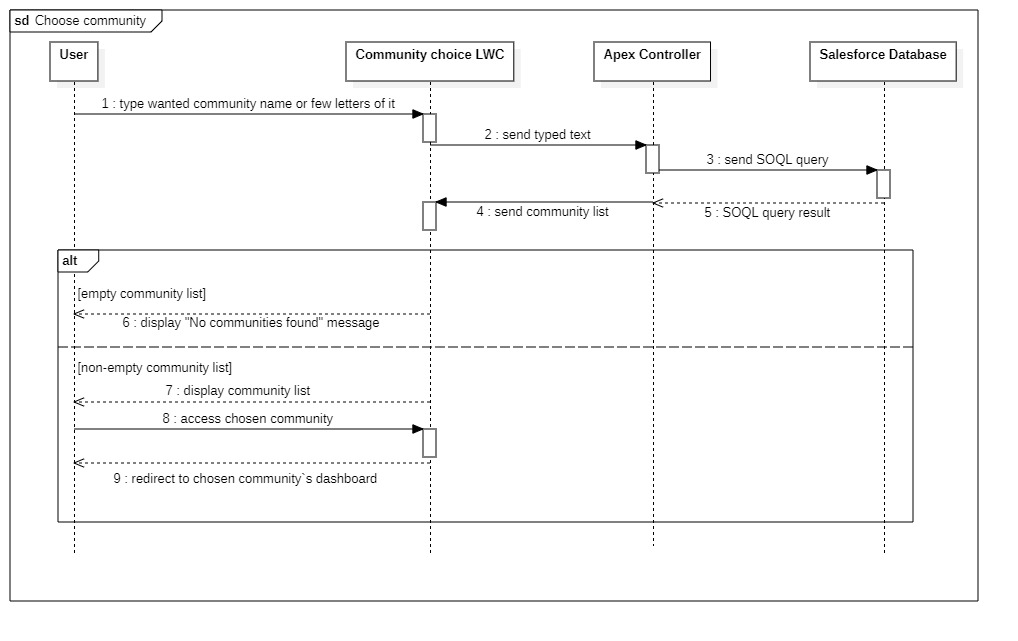
\includegraphics[scale=0.5]{Choose community_seq.jpg}
    \caption{Detailed sequence diagram of the "Choose community" use case}
\end{figure}
\subsection{Detailed sequence diagram of the "Access synthetic dashboard" use case}
The following figure illustrates the detailed sequence diagram of the use case
"Access synthetic dashboard".
This use case starts with opening a dashboard interface specific to the community chosen
by the user. The user may consult the account distribution chart, licenses distribution chart, login attempts distribution chart, time spent in community chart, and developers' error metrics chart where he will be able to select a specific user to monitor their error logs.
  \begin{figure}[H]%
    \center   
    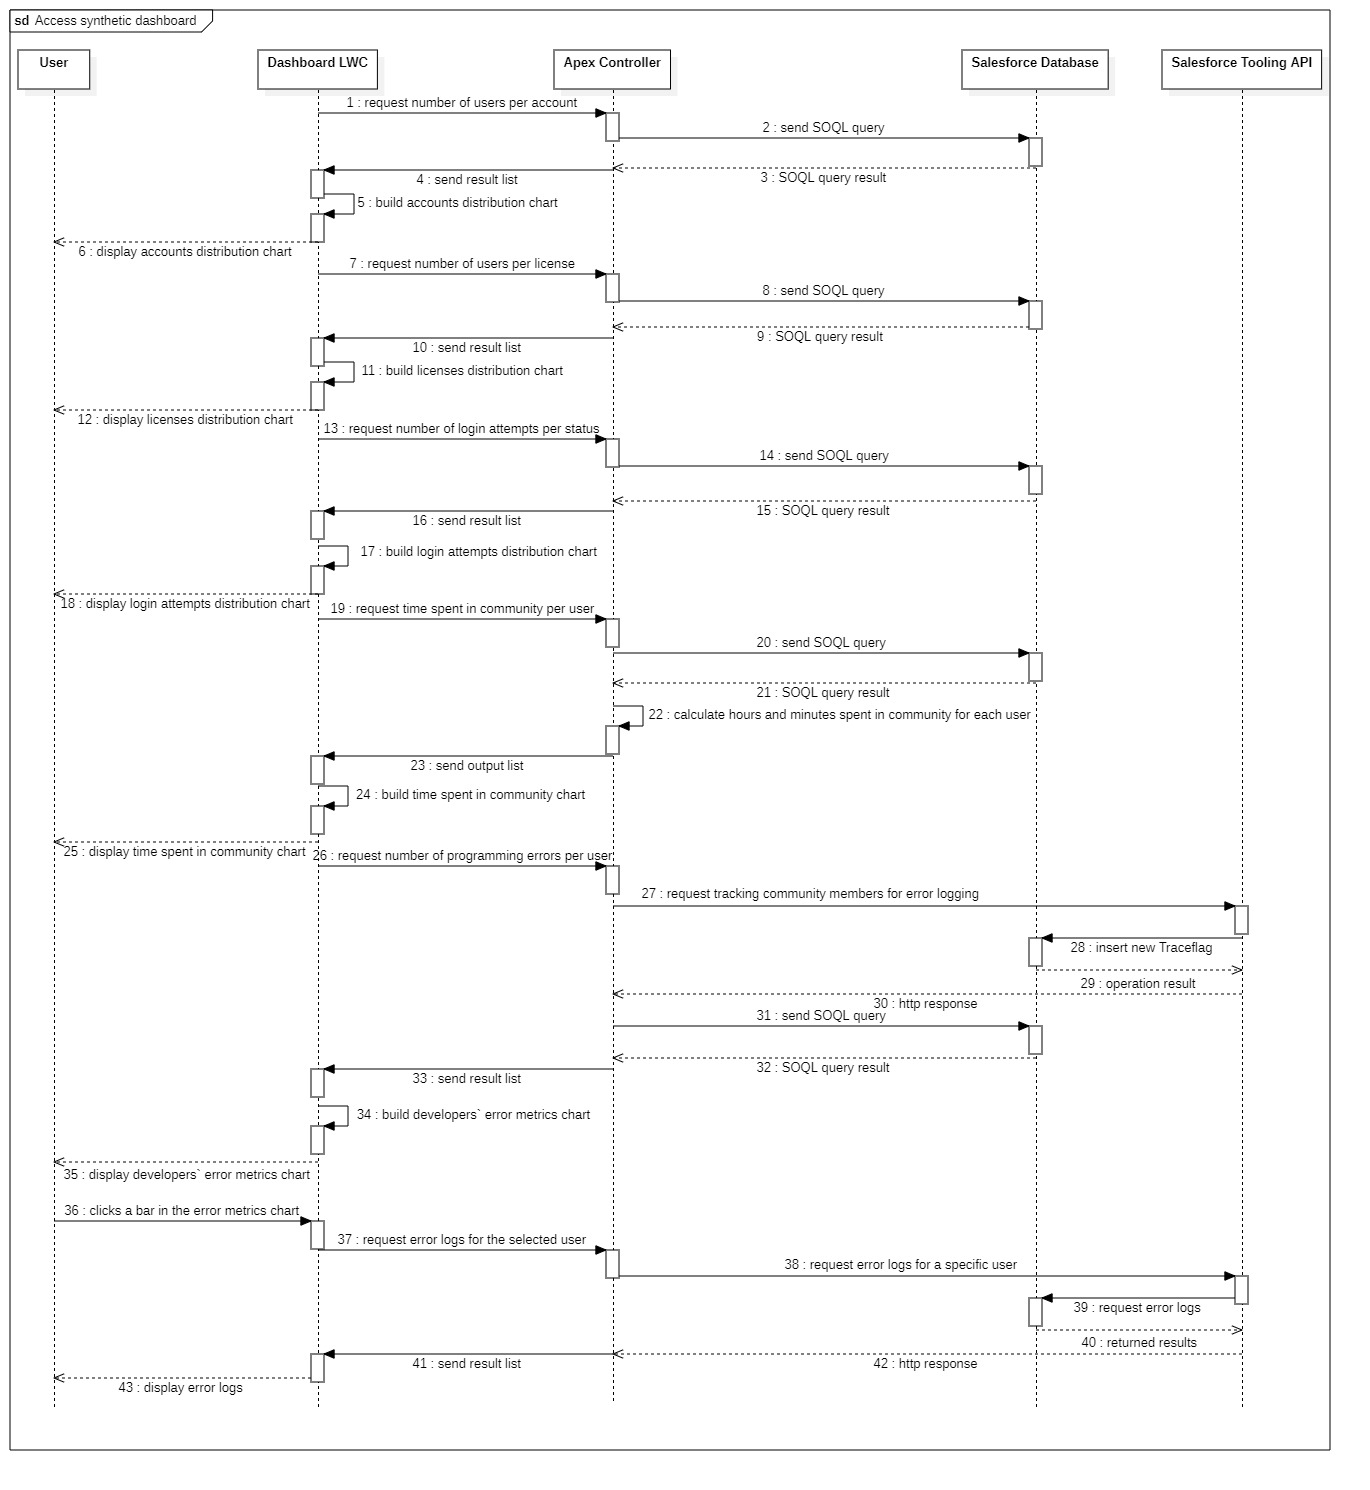
\includegraphics[scale=0.38]{Access synthetic dashboard_seq.jpg}
    \caption{Detailed sequence diagram of the "Access synthetic dashboard" use case}
\end{figure}

\subsection{Detailed sequence diagram of the "Consult users List" use case}
The following figure illustrates the detailed sequence diagram of the use case
"Consult users List".
This use case starts with opening an interface displaying a data table containing information about the user's community members. Then the user may search for a specific user using his Salesforce user name, full name, or his email address, he may also filter given results by account name, user status (active or not active), profile name, or account name. For the displayed members the user may choose to send welcome emails, send reset password emails to selected members as well as update their current status and their information.
 \begin{figure}[H]%
    \center   
    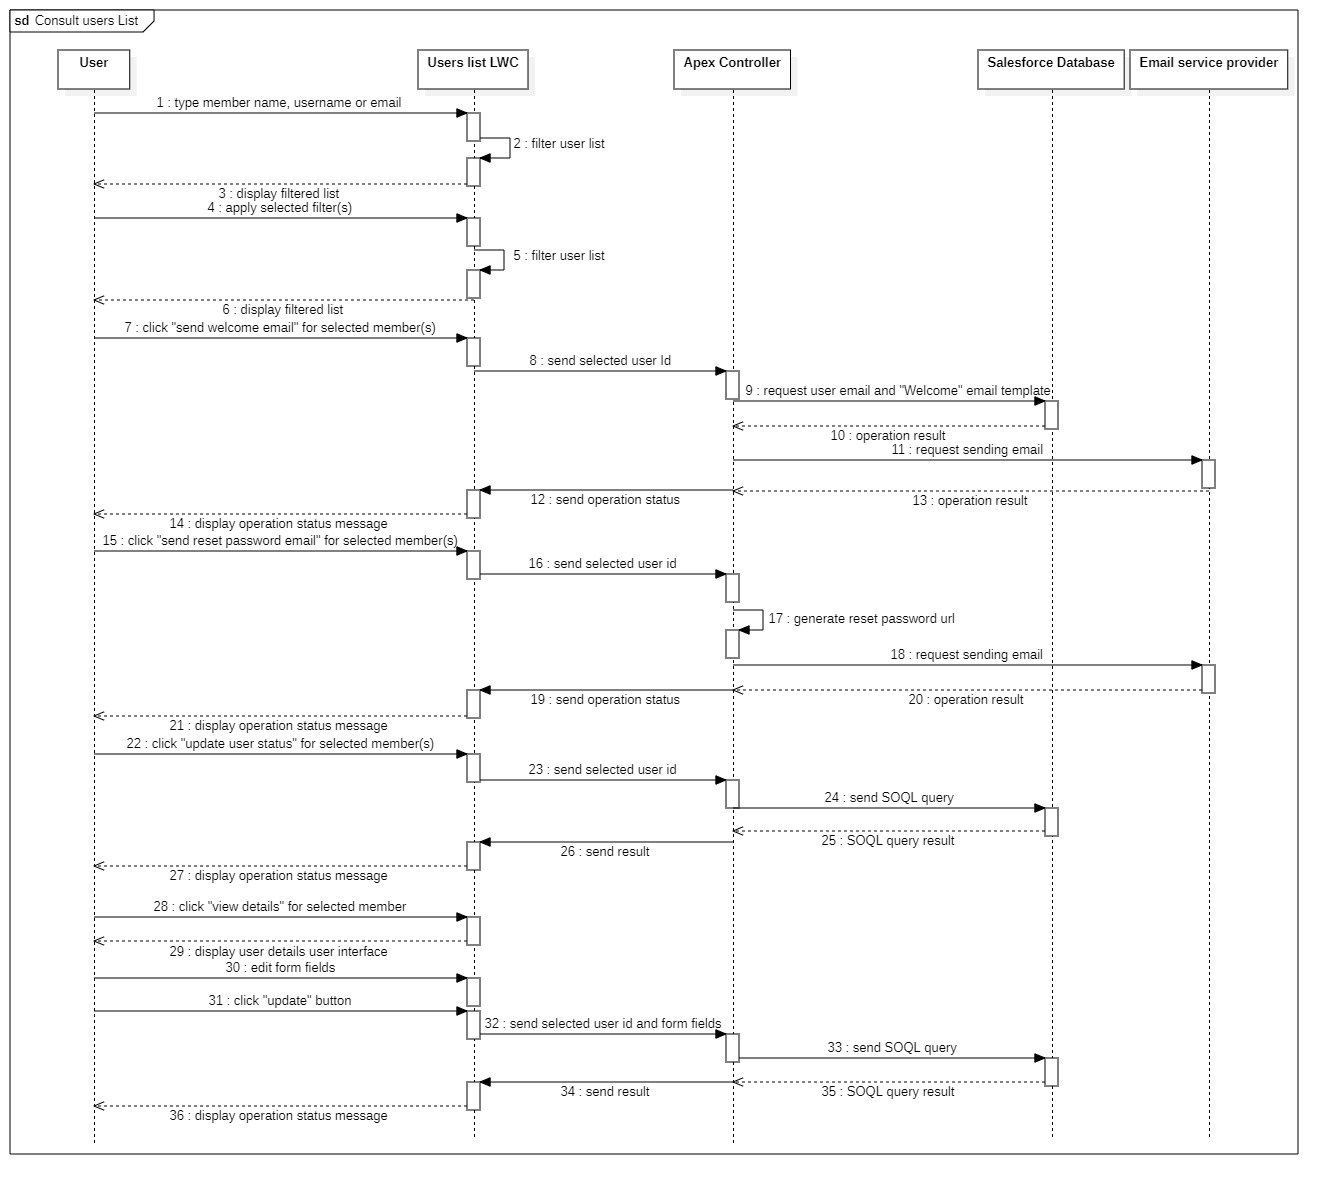
\includegraphics[scale=0.38]{Consult users List_seq.jpg}
    \caption{Detailed sequence diagram of the "Consult users List" use case}
\end{figure}
\subsection{Detailed sequence diagram of the "Add members" use case}
The following figure illustrates the detailed sequence diagram of the use case
"Add members".
This use case starts with opening an interface displaying an empty form containing input fields representing required and optional information about the new community member, the user may choose to add another empty form, add another form containing the same values as the previous one or delete the last form. Afterward, the user may choose to submit all forms where the system will prompt an error message in case one or more required fields are missing, the type user name already exists or the license limits are exceeded, otherwise, the system will prompt the success of the insert operation and will refresh the users' list. 
 \begin{figure}[H]%
    \center   
    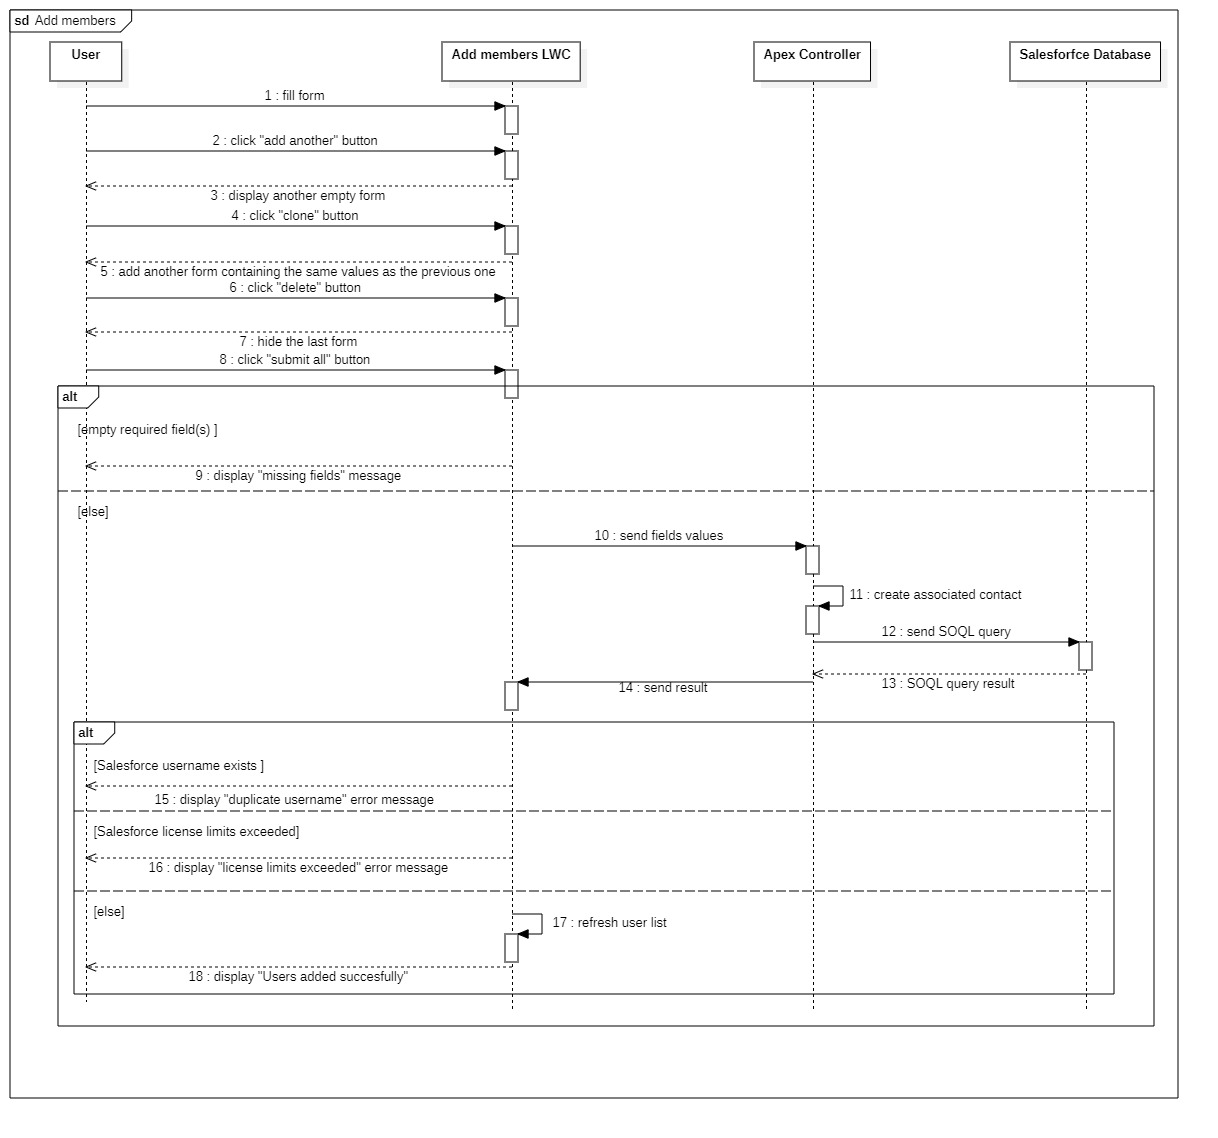
\includegraphics[scale=0.4]{Add members_seq.jpg}
    \caption{Detailed sequence diagram of the "Add members" use case}
\end{figure}

\subsection{Detailed sequence diagram of the "Consult failed login attempts" use case}
The following figure illustrates the detailed sequence diagram of the use case
"Consult failed login attempts".
This use case starts with opening an interface displaying a data table containing information about the failed login attempts committed by the user's community members. Then the user may search for a specific login event using the member's Salesforce user name or his full name, he may also filter given results by login event status (invalid password, no community access, etc) or by its date and time. For the displayed events the user may choose to send welcome security warning email to the concerned member or consult details about the full login event.
\begin{figure}[H]%
    \center   
    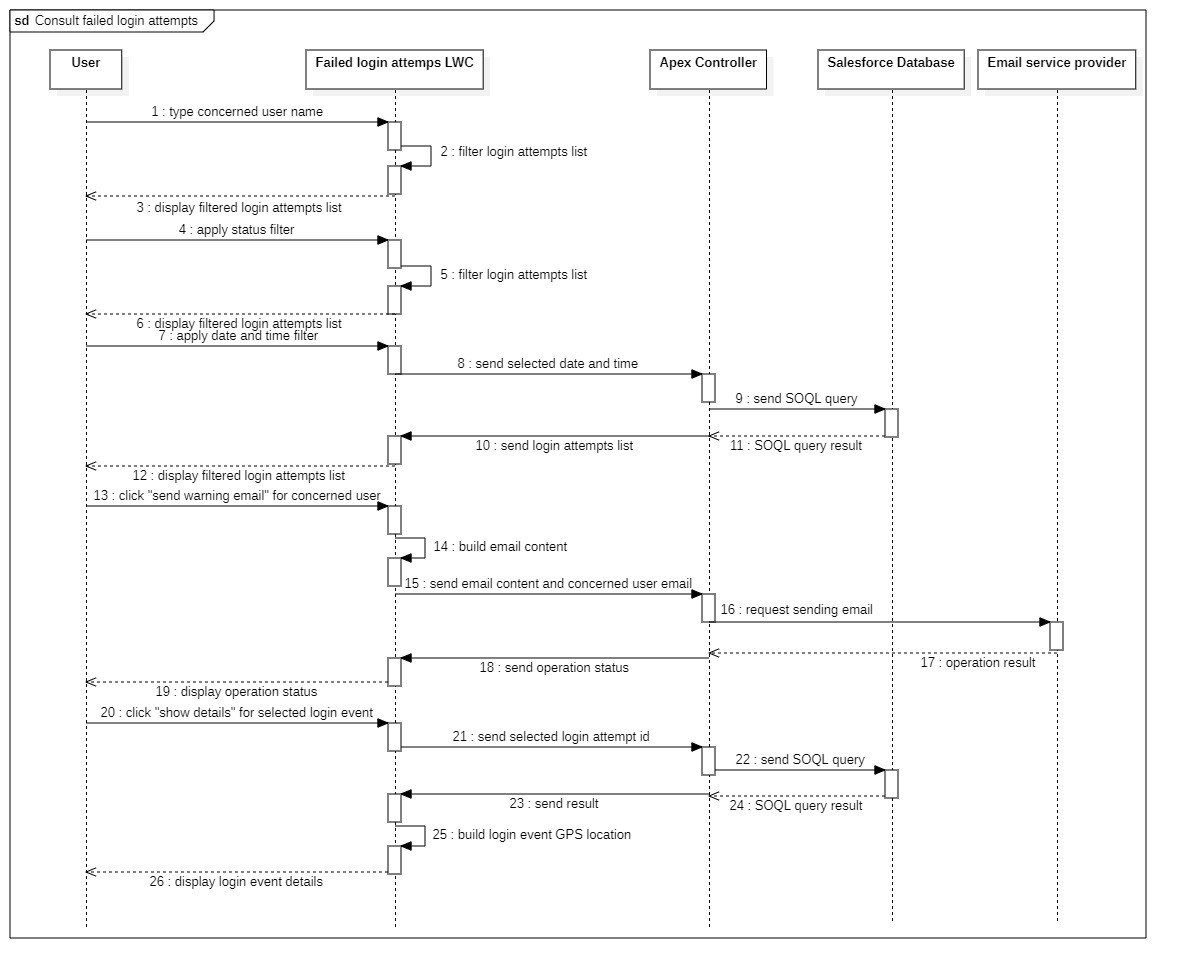
\includegraphics[scale=0.4]{Consult failed login attempts_seq.jpg}
    \caption{Detailed sequence diagram of the "Consult failed login attempts" use case}
\end{figure}
\subsection{Detailed sequence diagram of the "Consult connection history" use case}
The following figure illustrates the detailed sequence diagram of the use case
"Consult connection history".
This use case starts with opening an interface containing a bar chart displaying the number of logins for each member, the user may filter displayed results by date and time or by time range (yesterday, last week, or last month). For the displayed results the user may select a specific member to access further information about him where he will also be able to update his Salesforce user license.
\begin{figure}[H]%
    \center   
    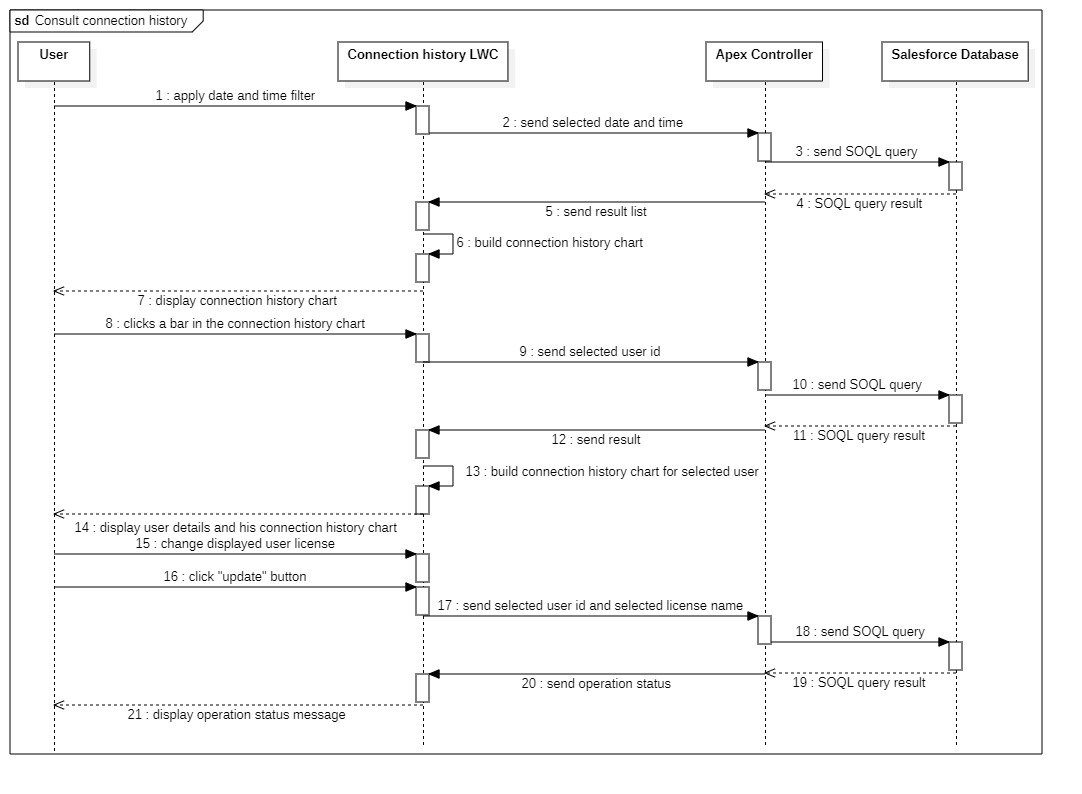
\includegraphics[scale=0.45]{Consult connection history_seq.jpg}
    \caption{Detailed sequence diagram of the "Consult connection history" use case}
\end{figure}
\subsection{Detailed sequence diagram of the "Access Chatbot" use case}
The following figure illustrates the detailed sequence diagram of the use case
"Access Chatbot".
This use case starts with opening a chat interface where the user may type any question that he wants to ask the digital assistant, he may also select one of the predefined questions proposed by the system, then the system will prompt the answer given by the Chatbot or display an error in case there is one. Next, the user will be asked for feedback regarding the given answer and he will be able to click the like or the dislike button, the given feedback will be saved in the current Salesforce organization database and will be exploited for future updates of the Chatbot.
\begin{figure}[H]%
    \center   
    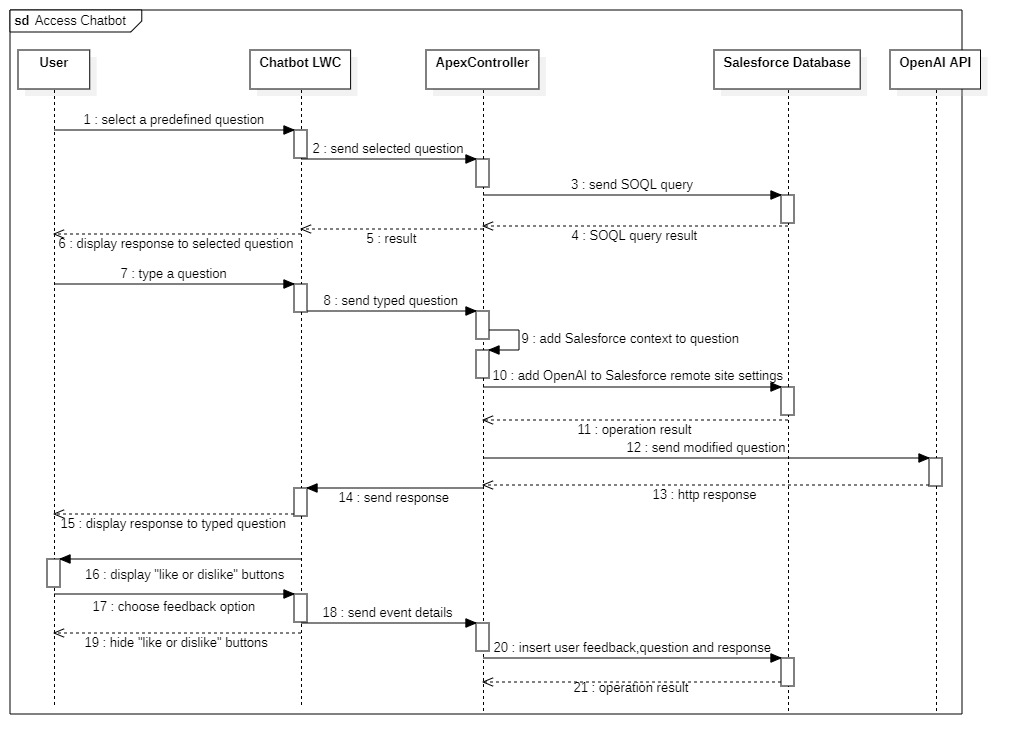
\includegraphics[scale=0.5]{Access Chatbot_seq.jpg}
    \caption{Detailed sequence diagram of the "Access Chatbot" use case}
\end{figure}
\section*{Conclusion}
This chapter presents one of the most important phases of the process of
development of a project: conception subdivided into the overall conception
and detailed conception.\\
We presented an MVC pattern and we
explained its application in our case. We have described the dynamic view
of the system through a set of sequence diagrams.\\
The following chapter will deal with the implementation of the project illustrated by screenshots of different interfaces. We will describe the environment of
work and the tools used too.
    \cleardoublepage%
    \chapter{Implementation}
\section*{Introduction}
In this chapter, we describe the working environment used during
the implementation of our application. We will also describe its physical layout using a deployment diagram. Then, we
detail the work carried out and the results obtained using a set
of screenshots representing the interfaces of the different features of
our app.
\section{Technical specification}
In this section, we will present the technical choices relating to
the hardware and software environment that contributed to the realization of our
application.
\subsection{Hardware environment}
During the different stages of our project, i.e. documentation,
code implementation and testing, we had:
\begin{itemize}
\item A laptop computer with the following configuration:
\begin{itemize}
\item Brand: Lenovo;
\item Processor: AMD Ryzen 3 3200U @ 2.60 GHz ;
\item Graphical processor:  Radeon Vega Mobile Gfx;
\item RAM: 12 GB;
\item Hard disk: 1TB;
\item System type: Windows 64-bit operating system.
\end{itemize} 
\item A desktop computer with the following characteristics:
\begin{itemize}
\item Brand: Lenovo;
\item Processor: Intel(R) Core(TM) i3-7100 CPU @ 3.90GHz 3.91GHz ;
\item Graphical processor: NVIDIA GeForce GT 1030
\item RAM: 8 GB;
\item Hard disk: 500 GB + 300 GB;
\item System type: Windows 64-bit operating system.
\end{itemize}
\end{itemize}
\subsection{Software environment}
Throughout the development phase, we used these software tools
and the following programming languages and frameworks:
\subsubsection{Software tools}
During the implementation of our project, we used the following software :
\paragraph*{Visual Studio Code}
Visual Studio Code is a popular source code editor developed by Microsoft. It provides a powerful and customizable environment for software development across various programming languages. Known for its lightweight design and extensive plugin ecosystem, Visual Studio Code offers features such as syntax highlighting, code completion, debugging capabilities, and version control integration. It supports multiple operating systems and offers a user-friendly interface.\\
Visual Studio Code allows mainly the JS/HTML/CSS files in our application as well as the XML configuration files for each LWC component, in addition to Cls files that represent the Apex Controllers and the files representing the Aura applications.
\begin{figure}[H]%
    \center   
    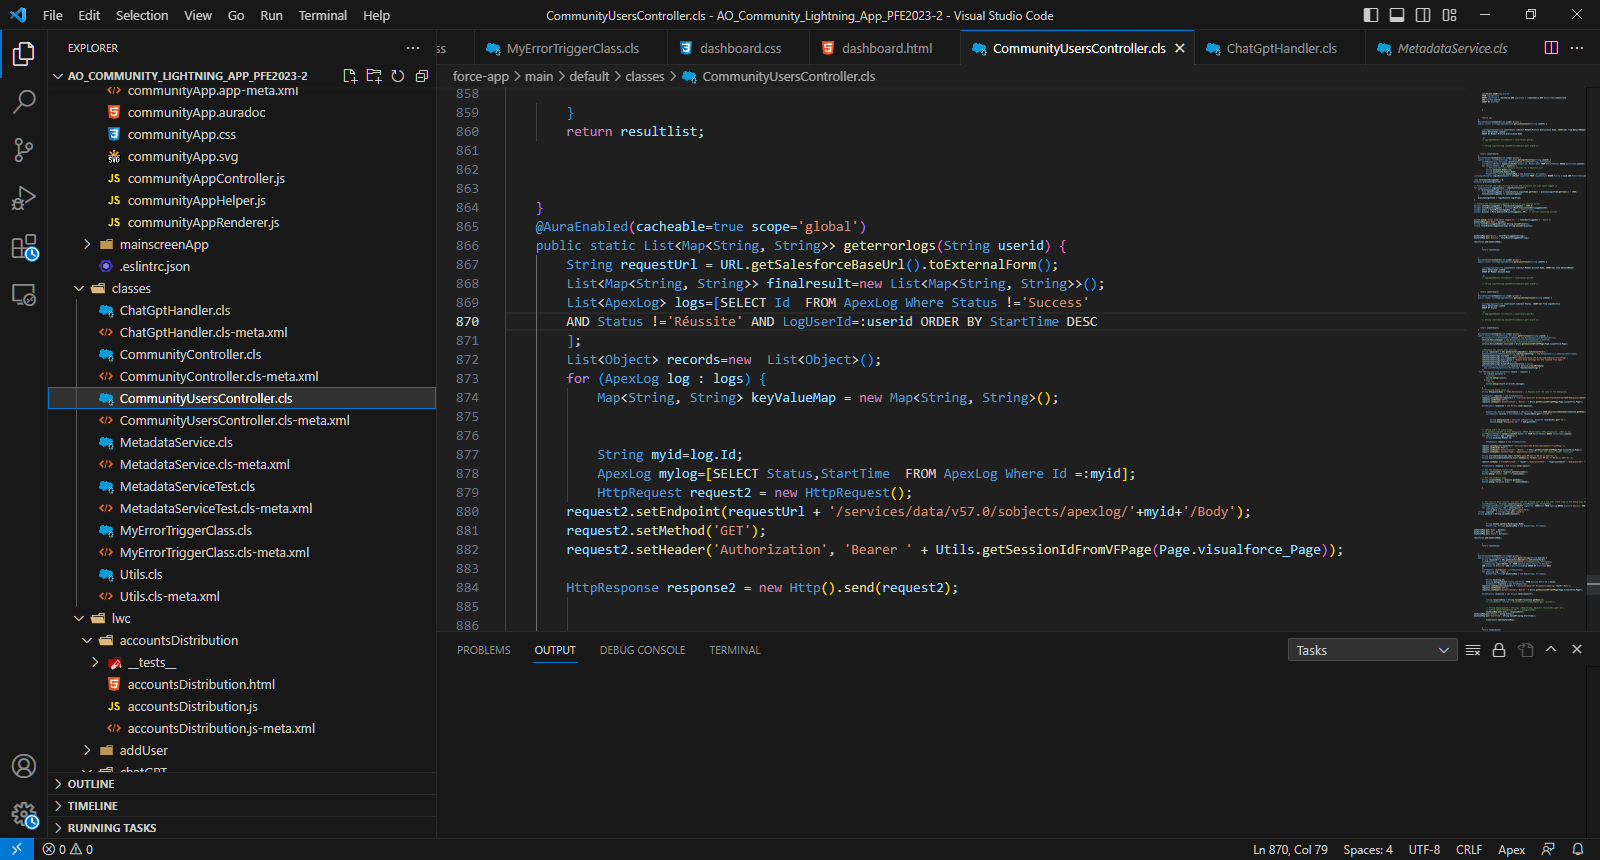
\includegraphics[scale=0.4]{vs.png}
    \caption{Visual Studio Code}
\end{figure}
\paragraph*{Salesforce Extension Pack for Visual Studio Code}
The Salesforce Development Extension Pack offers a collection of powerful tools specifically designed for developers working on the Salesforce platform. Integrated seamlessly with the lightweight and highly extensible VS Code editor, these tools empower developers with a comprehensive set of features tailored for various aspects of Salesforce development. With specialized functionalities for managing development orgs, including scratch orgs, sandboxes, and DE orgs, as well as robust support for Apex, Aura components, and Visualforce, the extension pack significantly enhances the development experience and productivity for Salesforce developers.
\begin{figure}[H]%
    \center   
    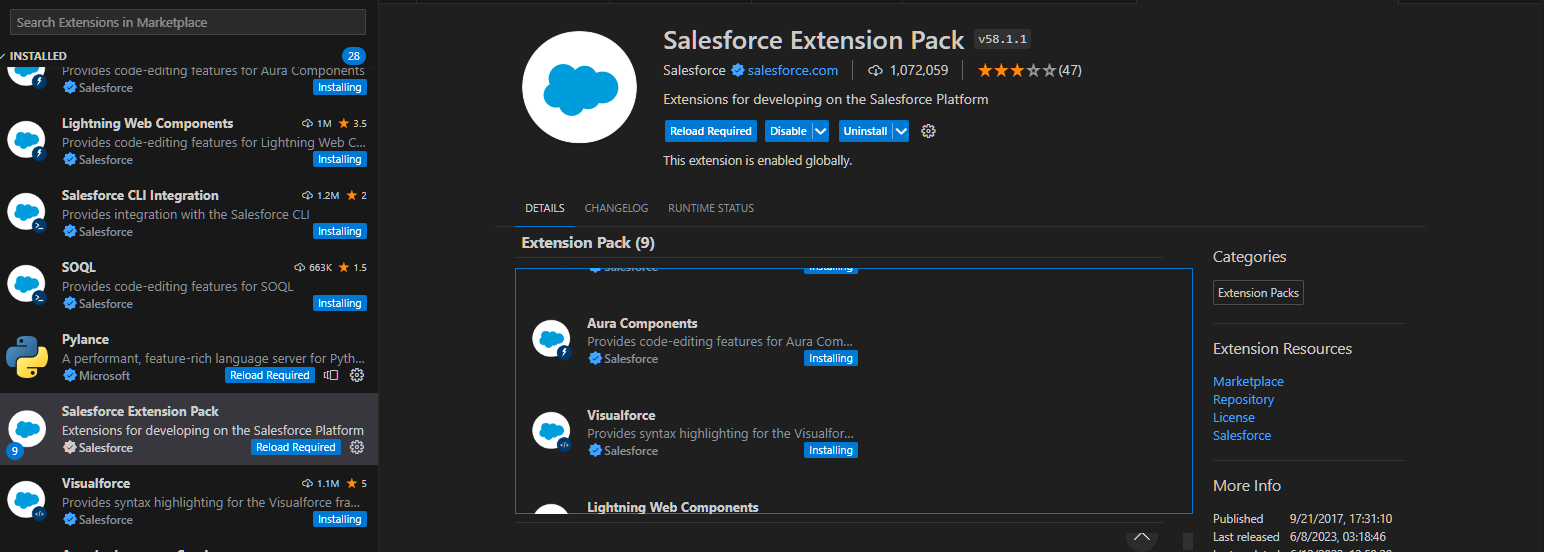
\includegraphics[scale=0.4]{extensions.png}
    \caption{Salesforce Extension Pack }
\end{figure}
\paragraph*{Salesforce CLI (sfdx)}
The Salesforce CLI is an essential command line interface that streamlines the development and automation processes for Salesforce orgs. It offers a wide range of capabilities, allowing developers to:
\begin{itemize}

\item[•] Consolidate Development Tools: By utilizing the Salesforce CLI, developers can bring together all the necessary tools required for efficient development and execute commands seamlessly within their Salesforce org.

\item[•] Source Synchronization: The CLI enables developers to synchronize source code between local environments and scratch orgs, ensuring that changes made in the development environment are accurately reflected in the org.

\item[•] Org Management: Developers can create and manage orgs effortlessly using the CLI. This includes provisioning new orgs, configuring various settings, and handling administrative tasks.

\item[•] Data Import and Export: With the CLI, developers can easily import and export data to and from their Salesforce orgs, facilitating data migration, data backup, and data integration processes.

\item[•] Test Creation and Execution: The CLI provides functionalities for creating and executing tests, allowing developers to ensure the quality and reliability of their code through automated testing procedures.

\item[•] Package Creation and Installation: Developers can utilize the CLI to create packages that encapsulate specific components or functionalities within their Salesforce orgs. These packages can be easily installed in other orgs, simplifying the deployment and distribution of applications.
\end{itemize}

\begin{figure}[H]%
    \center   
    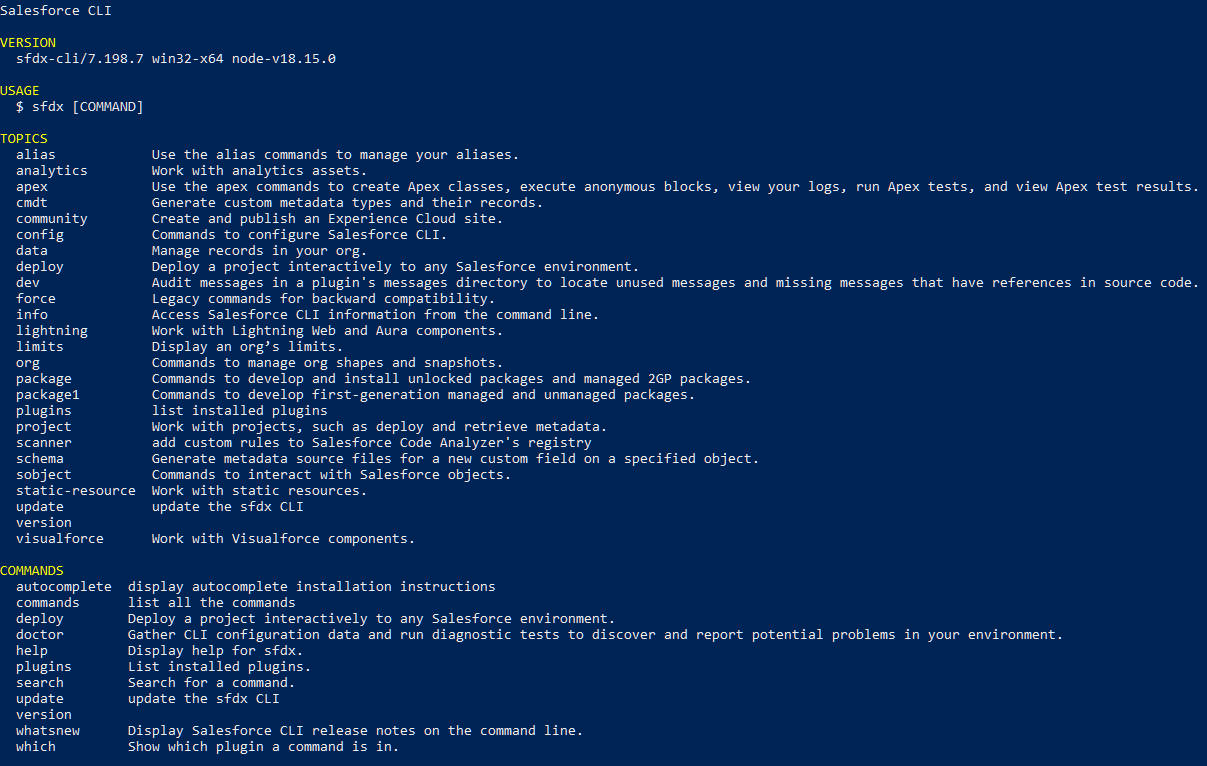
\includegraphics[scale=0.4]{cli.png}
    \caption{Salesforce CLI}
\end{figure}

\paragraph*{Salesforce Inspector}
Salesforce Inspector is a highly useful productivity tool designed specifically for Salesforce administrators and developers. It offers the capability to inspect data and metadata directly within the Salesforce user interface (UI), enhancing the efficiency and convenience of working with Salesforce.
With the added metadata layout, we were able to gain enhanced visibility and control over our Salesforce environment, making it easier to navigate, manipulate, and analyze data and metadata that is hidden by usual means.

\begin{figure}[H]%
    \center   
    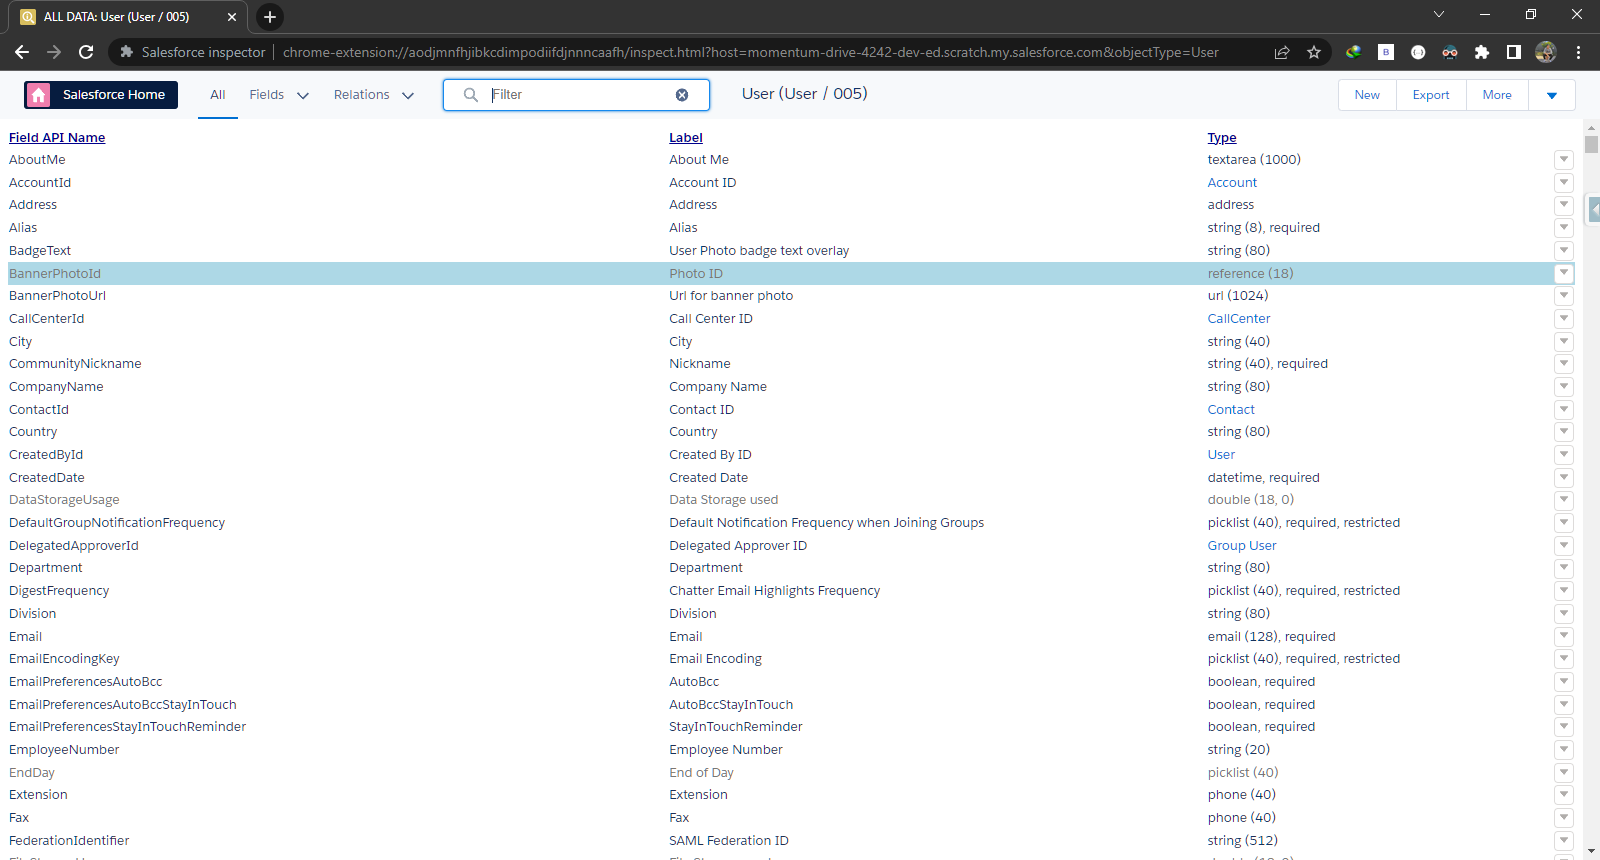
\includegraphics[scale=0.4]{inspector.png}
    \caption{Salesforce Inspector}
\end{figure}

\paragraph*{Maven Tools for Salesforce}
Maven Tools is an all-encompassing collection of Salesforce developer tools, purposefully designed to cater to the needs of Salesforce technical consultants. With its unique architecture, Maven Tools revolutionizes the delivery process of Salesforce implementations. This comprehensive toolkit offers a wide range of features, including an intelligent query editor, REST console, event hub, and much more, empowering developers to execute changes with increased speed and effectiveness.\\
In our application, we used Maven Tools for accessing the Salesforce tooling API.

\begin{figure}[H]%
    \center   
    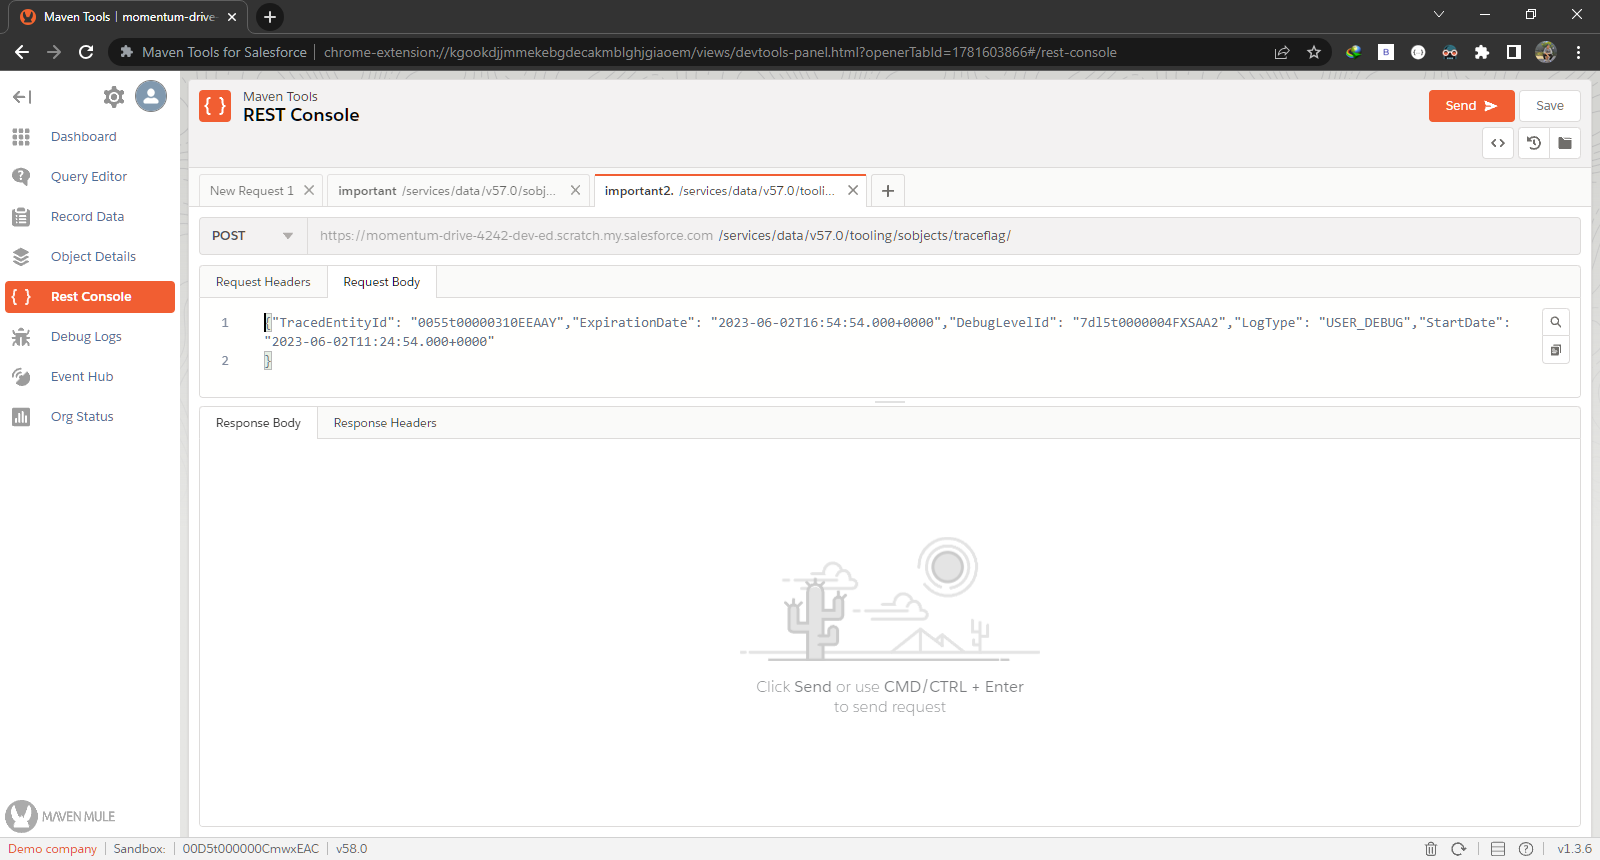
\includegraphics[scale=0.4]{maven.png}
    \caption{Maven Tools}
\end{figure}

\paragraph*{StarUML}
StarUML is a versatile software engineering tool designed for system modeling, employing various modeling notations including the Unified Modeling Language (UML), Systems Modeling Language (SysML), and classical modeling notations. Developed and published by MKLabs, StarUML offers comprehensive modeling capabilities and is compatible with Windows, Linux, and macOS operating systems.\\
In our application, we used StarUML to establish UML diagrams for this report.
\begin{figure}[H]%
    \center   
    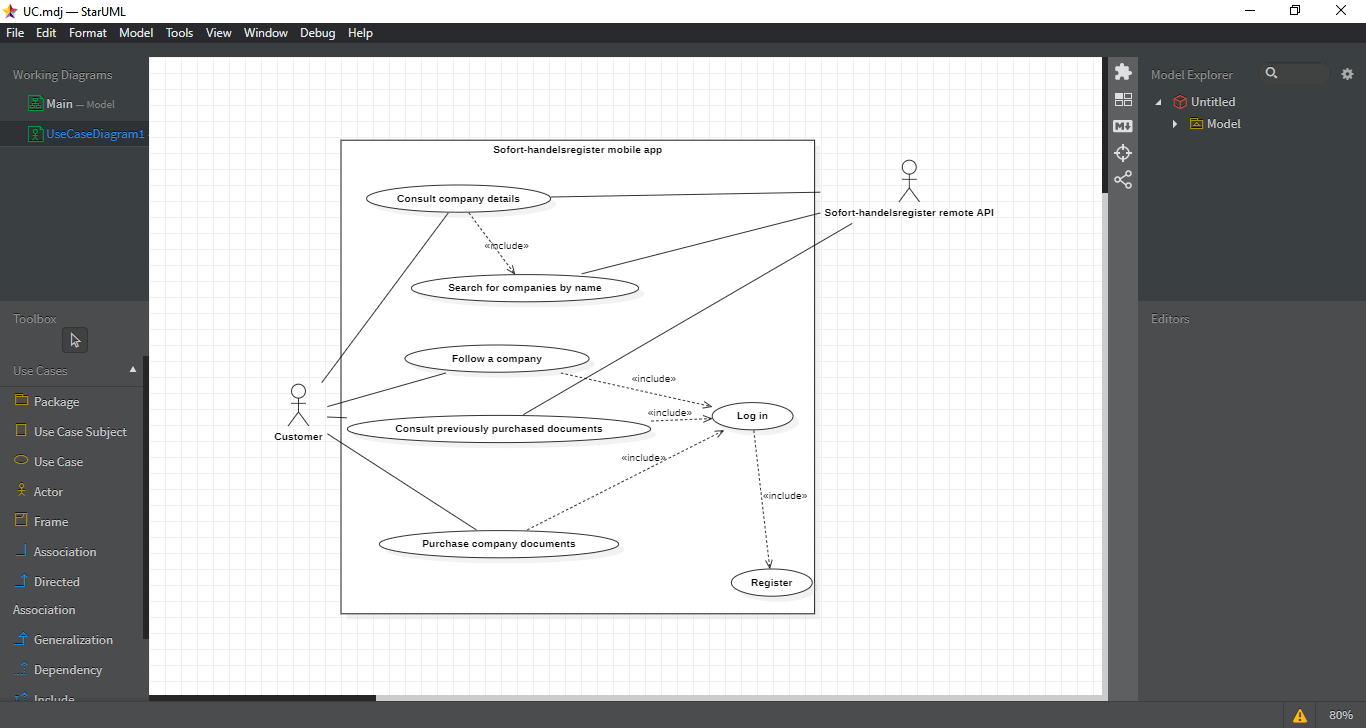
\includegraphics[scale=0.4]{star.png}
    \caption{StarUML}
\end{figure}
%current progress
\subsubsection{APIs and libraries}
\paragraph*{Salesforce Tooling API}
The Tooling API is a valuable resource for developers looking to create custom development tools or applications for Lightning Platform applications. It offers a range of capabilities that facilitate efficient and interactive development experiences.
One of the advantages of the Tooling API is its ability to retrieve smaller pieces of metadata using SOQL (Salesforce Object Query Language). This enables developers to fetch specific metadata components, resulting in improved performance compared to retrieving larger sets of metadata. \\
In our application, Salesforce tooling API was used to enable our application to interact with private Salesforce objects like Traceflag and DebugLevel.

\paragraph*{OpenAI API}
The OpenAI API is a versatile tool that can be utilized for a wide range of tasks involving natural language understanding and generation, as well as code-related operations. With its capabilities, the OpenAI API enables users to perform tasks such as language translation, text summarization, sentiment analysis, ChatBot development, and more.\\
In our application, OpenAI API was used to power up our Salesforce digital assistant and enable it to understand natural language.

\paragraph*{Libraries}
\begin{table}[H]
\begin{tabular}{|l|l|}
\hline
\textbf{Library}                                                       & \textbf{Usage}                                                                                                                                                                     \\ \hline
\begin{tabular}[c]{@{}l@{}}Salesforce \\ Metadata Service\end{tabular} & \begin{tabular}[c]{@{}l@{}}- Automate remote site settings configuration.\\ - Automate custom Salesforce object for chatbot feedback.\end{tabular}                                 \\ \hline
LWC's wire                                                             & \begin{tabular}[c]{@{}l@{}}- Establish a connection between the lightning web component \\ and an Apex method, a function in a JavaScript module, or a wire adapter.\end{tabular} \\ \hline
LWC's API & - Create a public property or method that can be accessed by parent components.                                                                                                    \\ \hline
Chart Js                                                               & - Build responsive and interactive charts from given Salesforce data.                                                                                                              \\ \hline
\end{tabular}
\caption{Libraries}
\end{table}
\subsubsection{Programming languages and frameworks}
\paragraph*{Apex}
Apex is a strongly typed, object-oriented programming language that allows developers to execute flow and transaction control statements on Salesforce servers in conjunction with calls to the API. Using syntax that looks like Java and acts like database stored procedures, Apex enables developers to add business logic to most system events, including button clicks, related record updates, and Visualforce pages. Apex code can be initiated by Web service requests and from triggers on objects.\cite{8}
\paragraph*{LWC(Lightning Web Components)}
Lightning Web Components is a framework that leverages core Web Components standards and focuses on delivering optimal performance within Salesforce-supported browsers. By utilizing the native capabilities of modern browsers, Lightning Web Components achieves a lightweight structure that excels in performance. It primarily utilizes standard JavaScript, HTML, and CSS, making it accessible and familiar to those already experienced in web development.
\paragraph*{Aura}
Aura components are the self-contained and reusable units of an app. They represent a reusable section of the UI and can range in granularity from a single line of text to an entire app.
The framework includes a set of prebuilt components. For example, components that come with the Lightning Design System styling are available in the lightning namespace.\cite{9}
\paragraph*{SOQL}
SOQL (Salesforce Object Query Language) serves as a powerful query language dedicated to retrieving data from Salesforce databases. While sharing similarities with SQL (Structured Query Language), SOQL is specifically designed for querying Salesforce data.
Using SOQL, developers can efficiently query and retrieve data from both standard and custom objects within the Salesforce platform. This includes accessing records, and fields, and establishing relationships between different objects. 
\paragraph*{SLDS}
The Salesforce Lightning Design System (SLDS) represents a comprehensive set of guidelines and resources offered by Salesforce to easily create visually consistent and user-friendly interfaces within Salesforce applications.
It also provides developers with a rich assortment of CSS styles, design patterns, and components. These resources can be utilized to construct custom Salesforce applications, including Lightning Web Components (LWC) and Aura components.
\paragraph*{XML}
The XML (Extensible Markup Language) allows the developer to create and share information formats via networks. This standard is used to describe data in our application as well as configure component visibility in Salesforce.
\paragraph*{JSON}
JSON(JavaScript Object Notation) is a lightweight data-interchange format that is easy to read and write and
frequently used by developers. Within our application, it was mainly used for communicating with external APIs. 
\subsection{Deployment diagram of the application}
The deployment diagram models the physical architecture of a system.
This diagram shows the topology of the software elements that are deployed over the material elements.
The following figure represents the deployment diagram of our application.
\begin{figure}[H]%
    \center   
    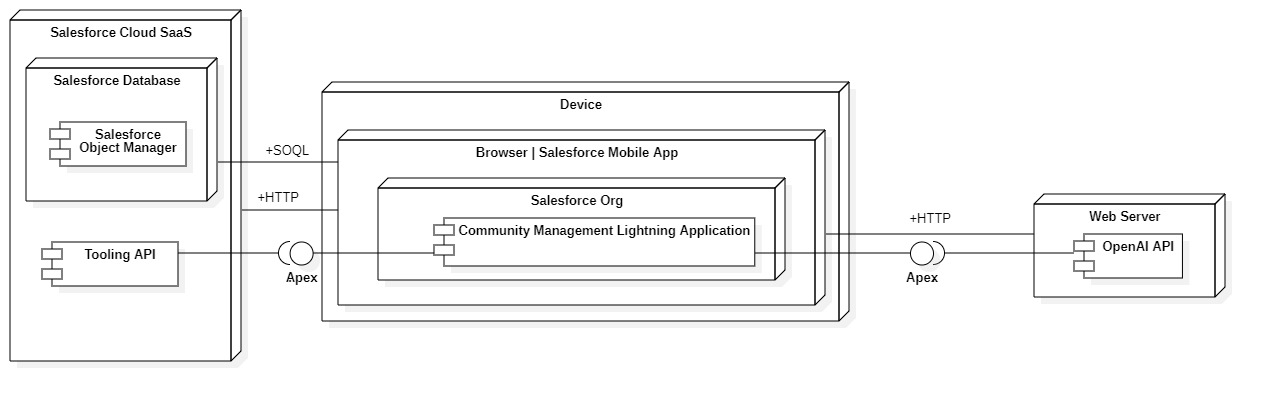
\includegraphics[scale=0.4]{DeploymentDiagram.jpg}
    \caption{Deployment diagram of the application}
\end{figure}
Our application's deployment diagram is composed of 3 Nodes:
\begin{itemize}
\item Device: the physical device that is used to access the user's Salesforce org containing our lightning application
\item Web Server: the web server embedding the OpenAI API responsible for powering up our ChatBot 
\item Salesforce cloud SAAS(software as a service): the provider of the Salesforce database that enables our application to create, read, update, or delete Salesforce records' data and the provider of the tooling API that enables our application to automate org configuration and similar operation.  
\end{itemize}
The interactions between software components are:
\begin{itemize}
\item[•] between our application and OpenAI API via HTTP requests. The exchange of data is in JSON format through the
REST(representational state transfer) APIs, the resulting data is exploited through Apex.
\item[•] between our application and Salesforce Database via SOQL queries. The exchange of data is in sObjects (Salesforce objects) format.
\item[•] between our application and Tooling API via HTTP requests. The exchange of data is in JSON format through the
REST(representational state transfer) APIs, the resulting data is exploited through Apex.

\end{itemize}

\section{Application interfaces}
In this part, we present the different features of our
application by presenting the graphical interfaces produced:
\subsection{Launching the application}
The following figure represents the landing page of the application where the user can choose to access one of his owned communities or search for a specific one by its name using the provided search bar.
\begin{figure}[H]%
    \center   
    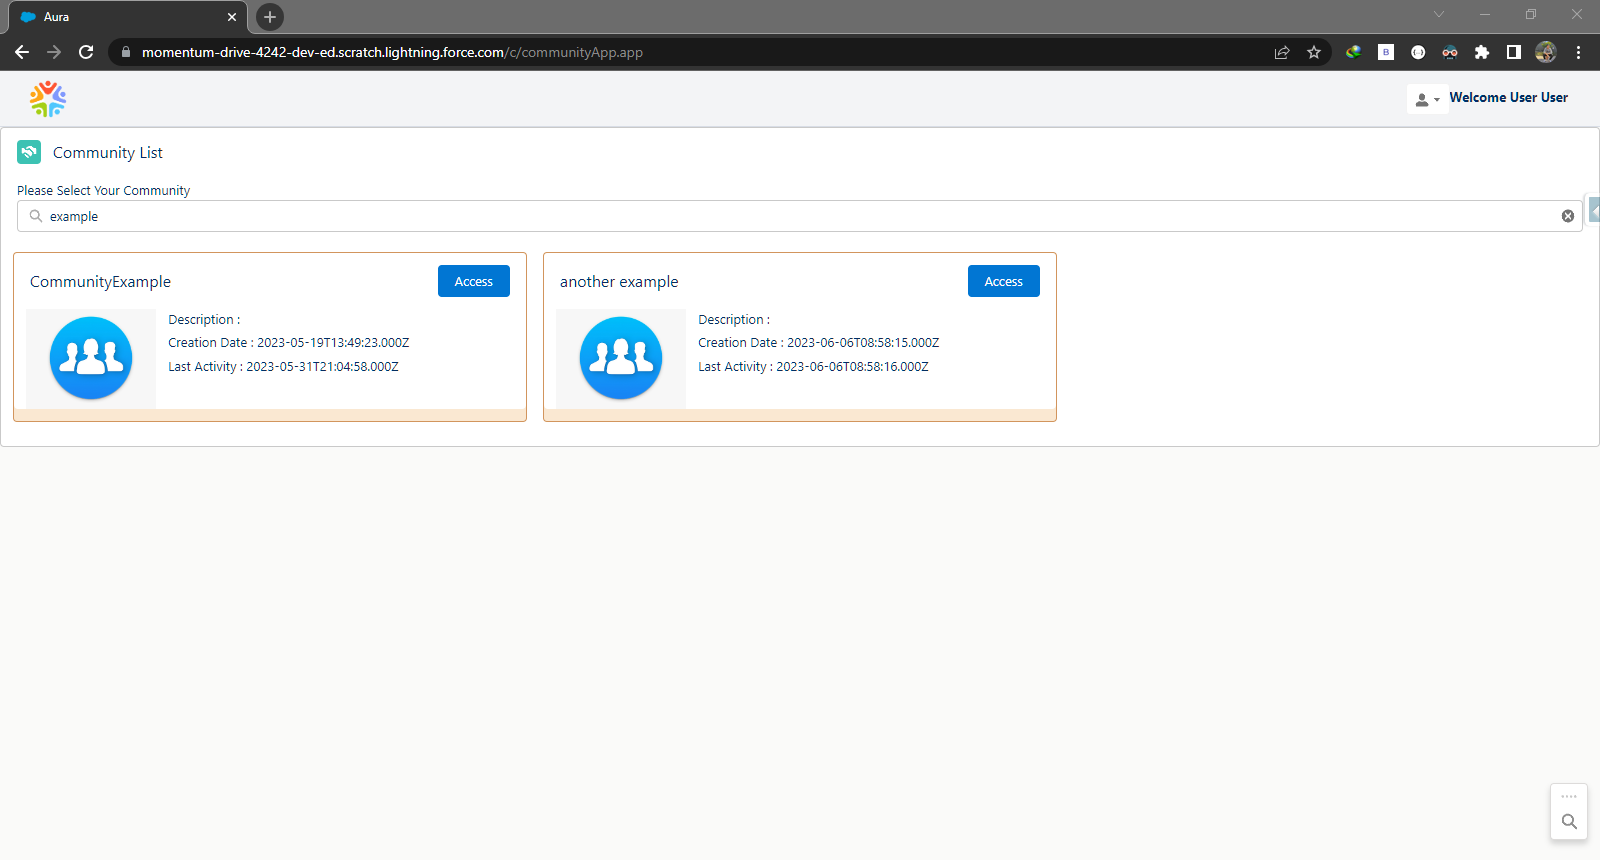
\includegraphics[scale=0.4]{home.png}
    \caption{Community selection interface (landing page of the application)}
\end{figure}
\subsection{Community Dashboard}
The following figure represents the community dashboard, that shows up upon accessing the selected community bu the user, containing KPIs charts that help the user monitor his community.\\
The following figure represents respectively the accounts distribution chart, Salesforce user licenses distribution chart, and login attempts status distribution chart for the current community.
\begin{figure}[H]%
    \center   
    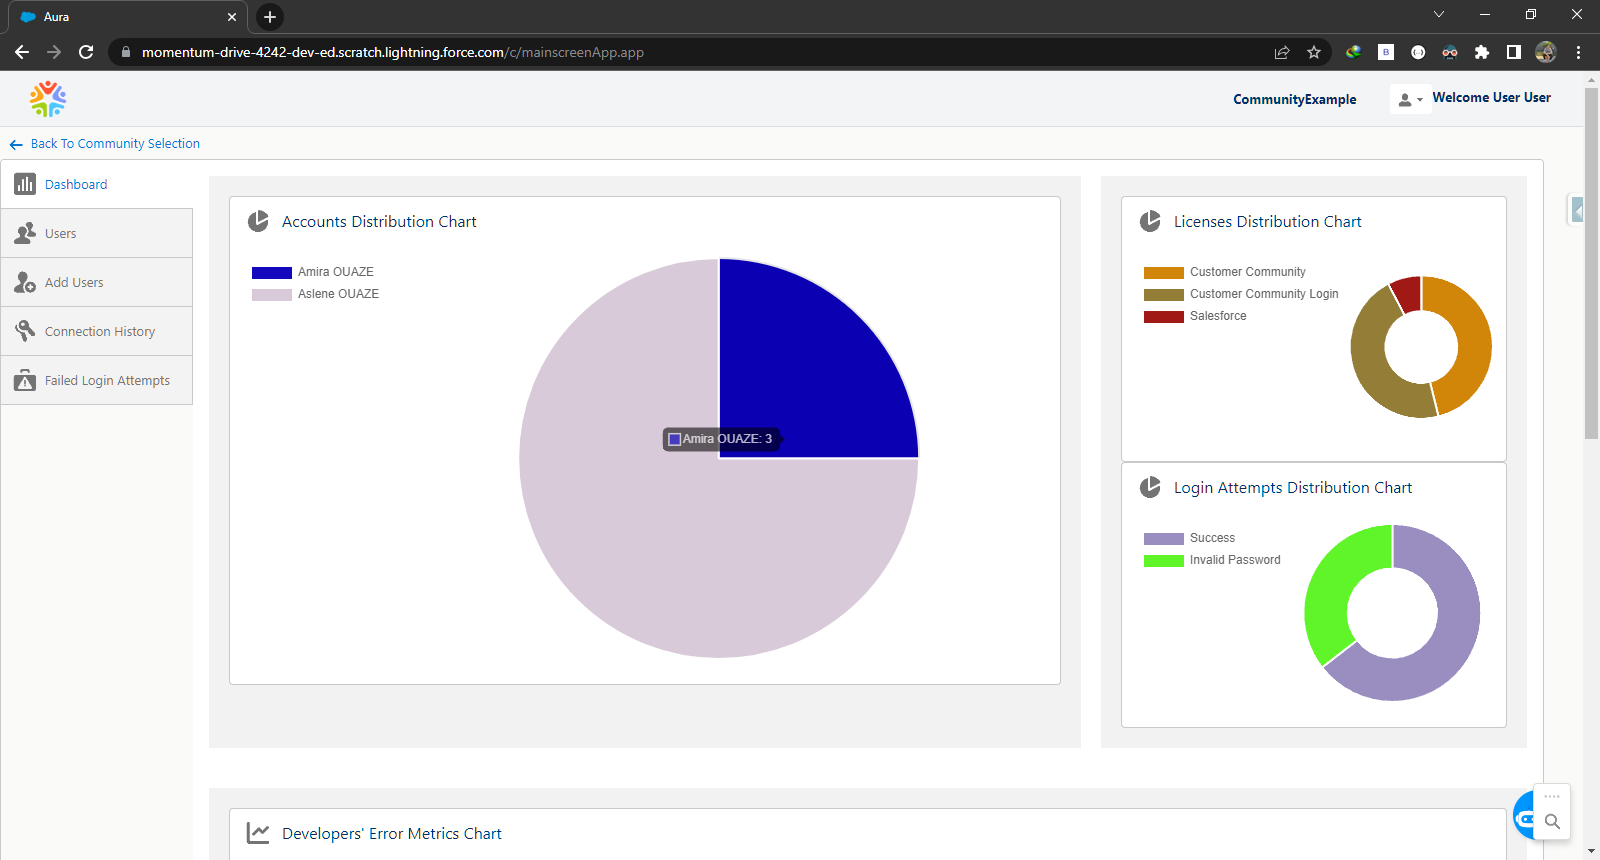
\includegraphics[scale=0.4]{dashboard1.png}
    \caption{Community dashboard interface (distribution charts)}
\end{figure}
The following figure represents the time spent in the community chart that shows the number of hours and minutes spent by each member when surfing the current community.
\begin{figure}[H]%
    \center   
    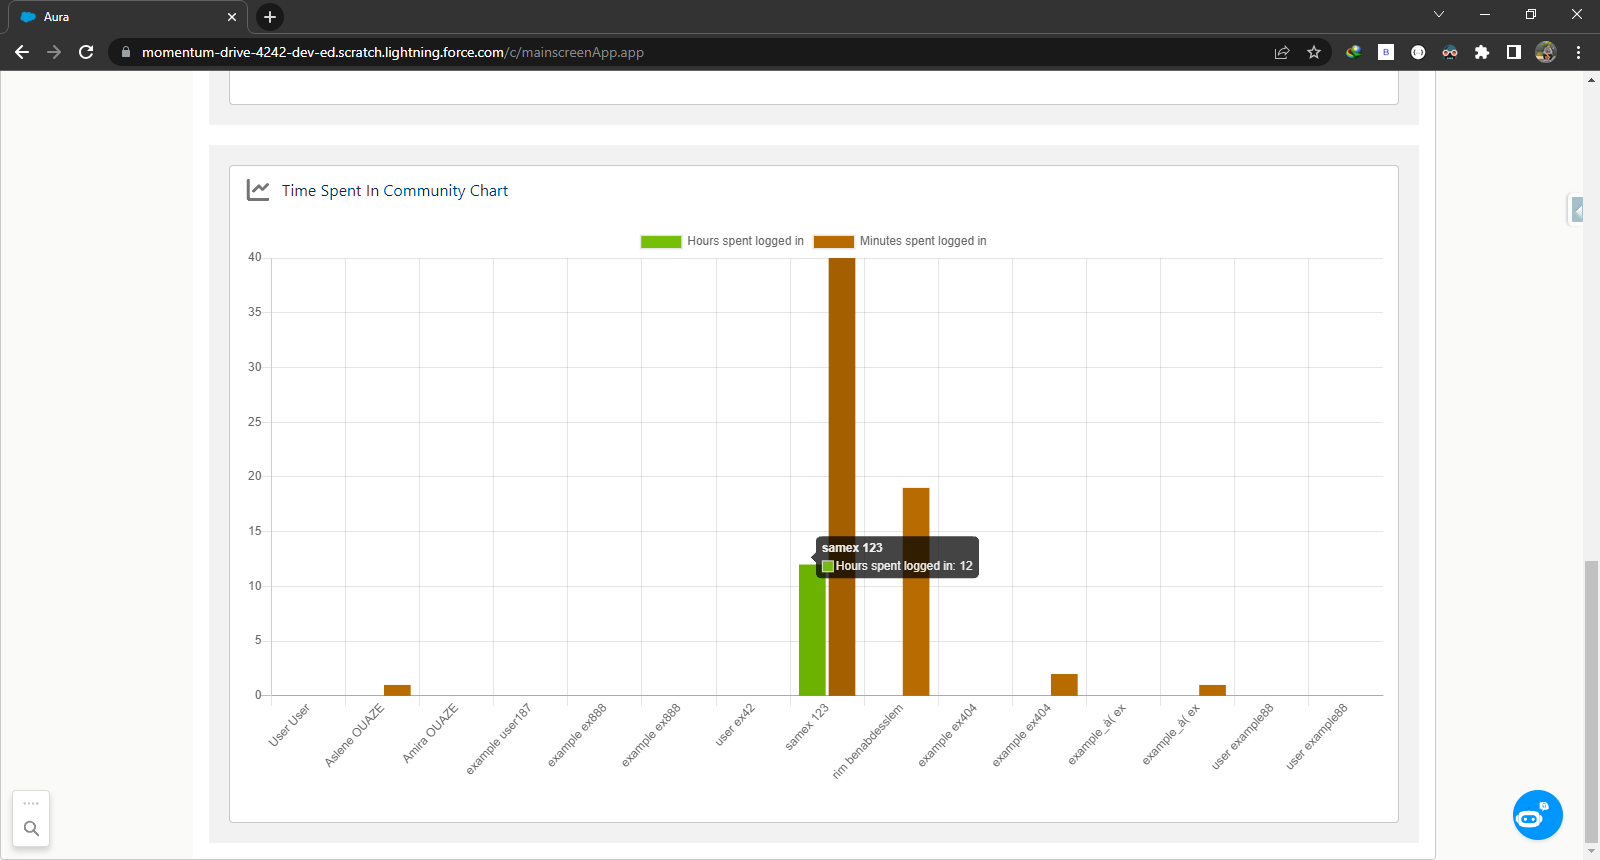
\includegraphics[scale=0.4]{dashboard2.png}
    \caption{Community dashboard interface (time spent in the community chart)}
\end{figure}
The following figure represents the community developers' error metrics chart that shows the number of programming errors faced by each developer working in the current community.
\begin{figure}[H]%
    \center   
    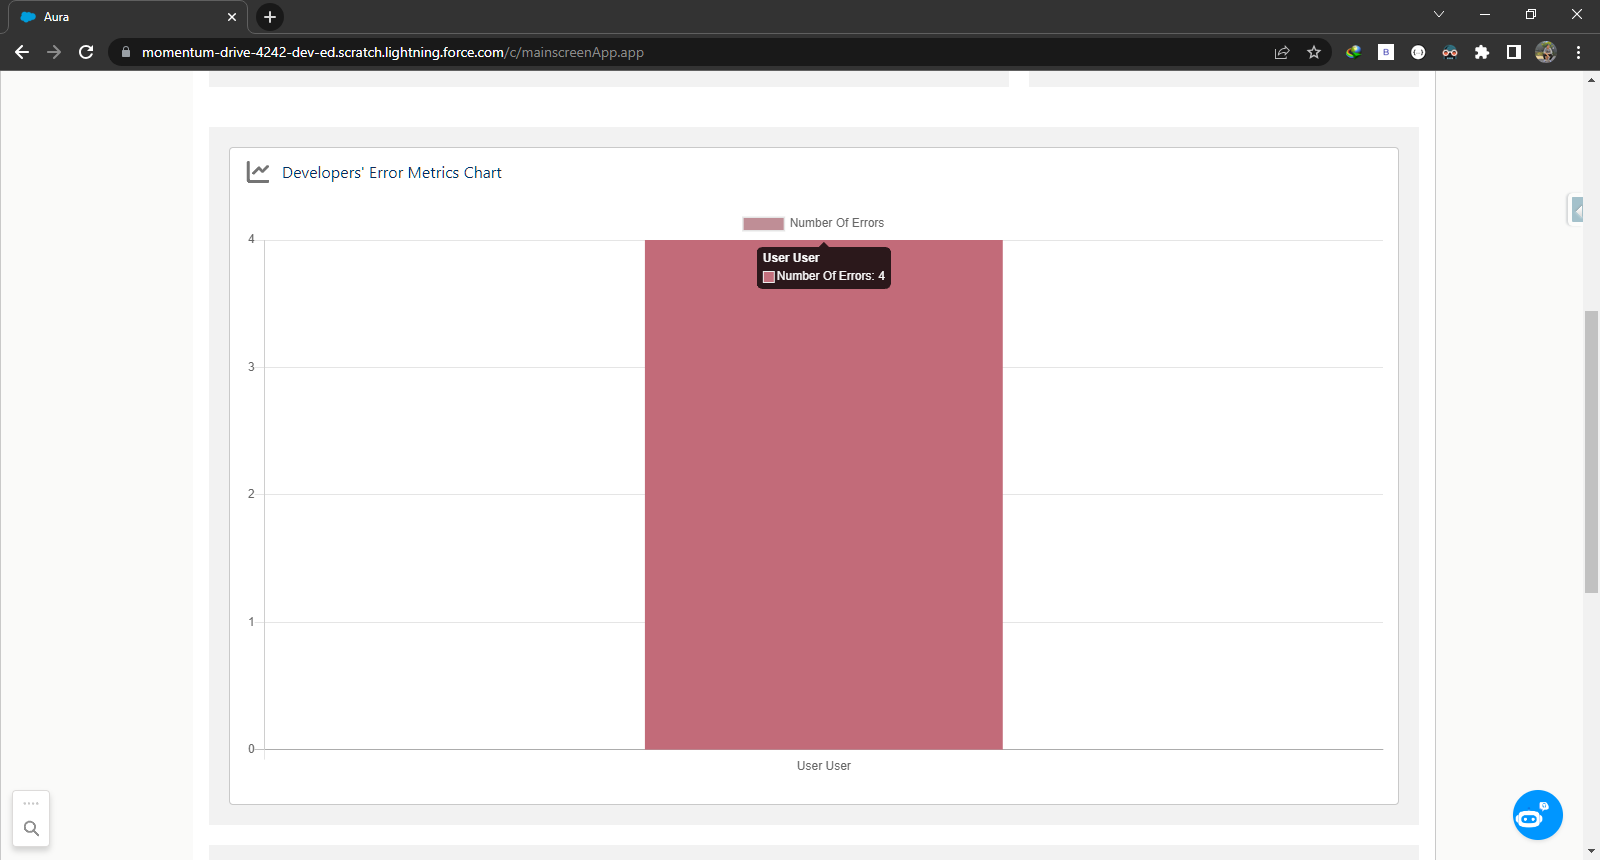
\includegraphics[scale=0.4]{dashboard3.png}
    \caption{Community dashboard interface (developers' error metrics chart)}
\end{figure}
Upon clicking on one of the bars displayed in the previous chart the complete error logs specific to the selected developer will be displayed as shown in the following figure.
\begin{figure}[H]%
    \center   
    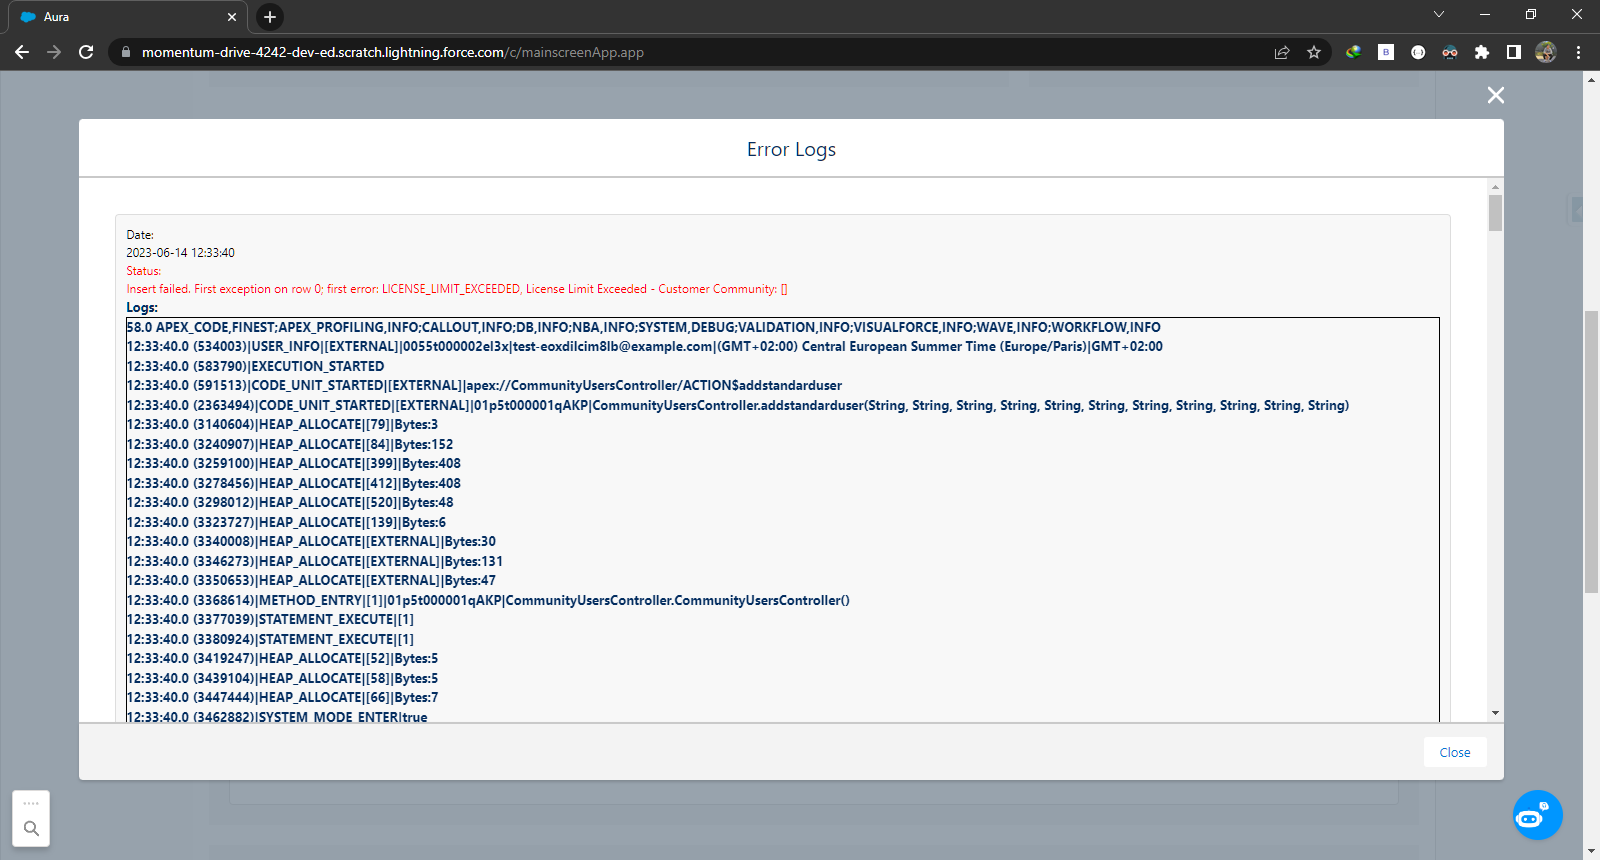
\includegraphics[scale=0.4]{dashboard4.png}
    \caption{Community developer error logs interface}
\end{figure}
\subsection{User list }
The following figure represents the community members list where the user can navigate through his community members' information using given pagination options. He may also filter displayed members by user status (active or inactive), account name, or profile label using the given combo boxes or search for a specific user using his Salesforce user name, full name, or email using the provided search bar. The user can perform actions on one or multiple members, these actions can be activating/deactivating selected members, sending welcome emails to selected members, or sending reset password reset emails to selected members. 

\begin{figure}[H]%
    \center   
    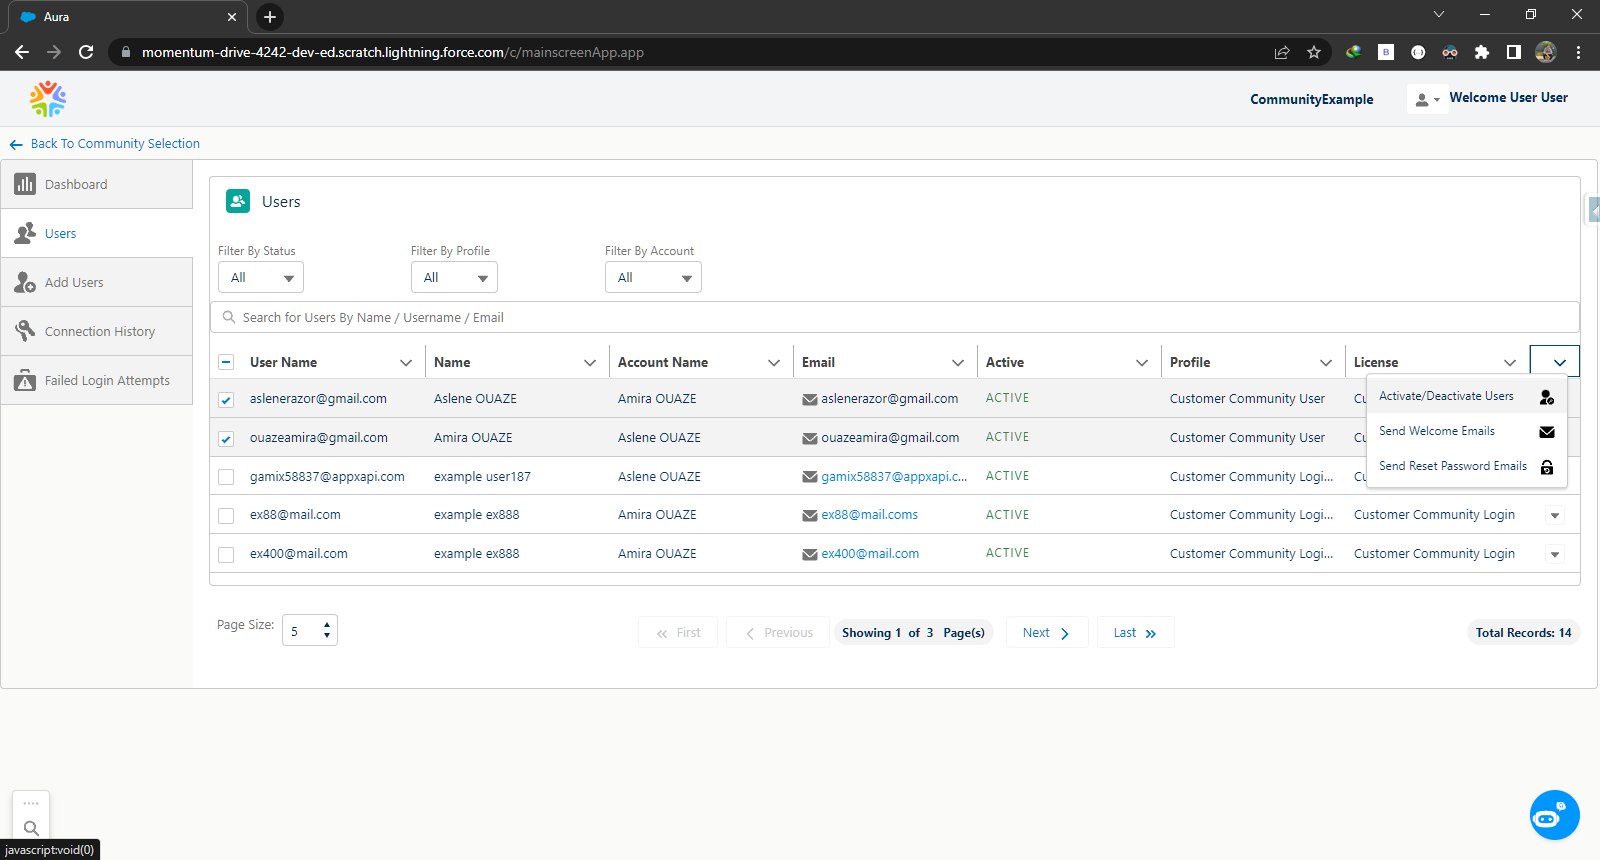
\includegraphics[scale=0.4]{userlist1.png}
    \caption{User list interface}
\end{figure}
The user may also consult details about a specific user as well as update said details as shown in the following figure, the show details action is only selectable when selecting one community member.
\begin{figure}[H]%
    \center   
    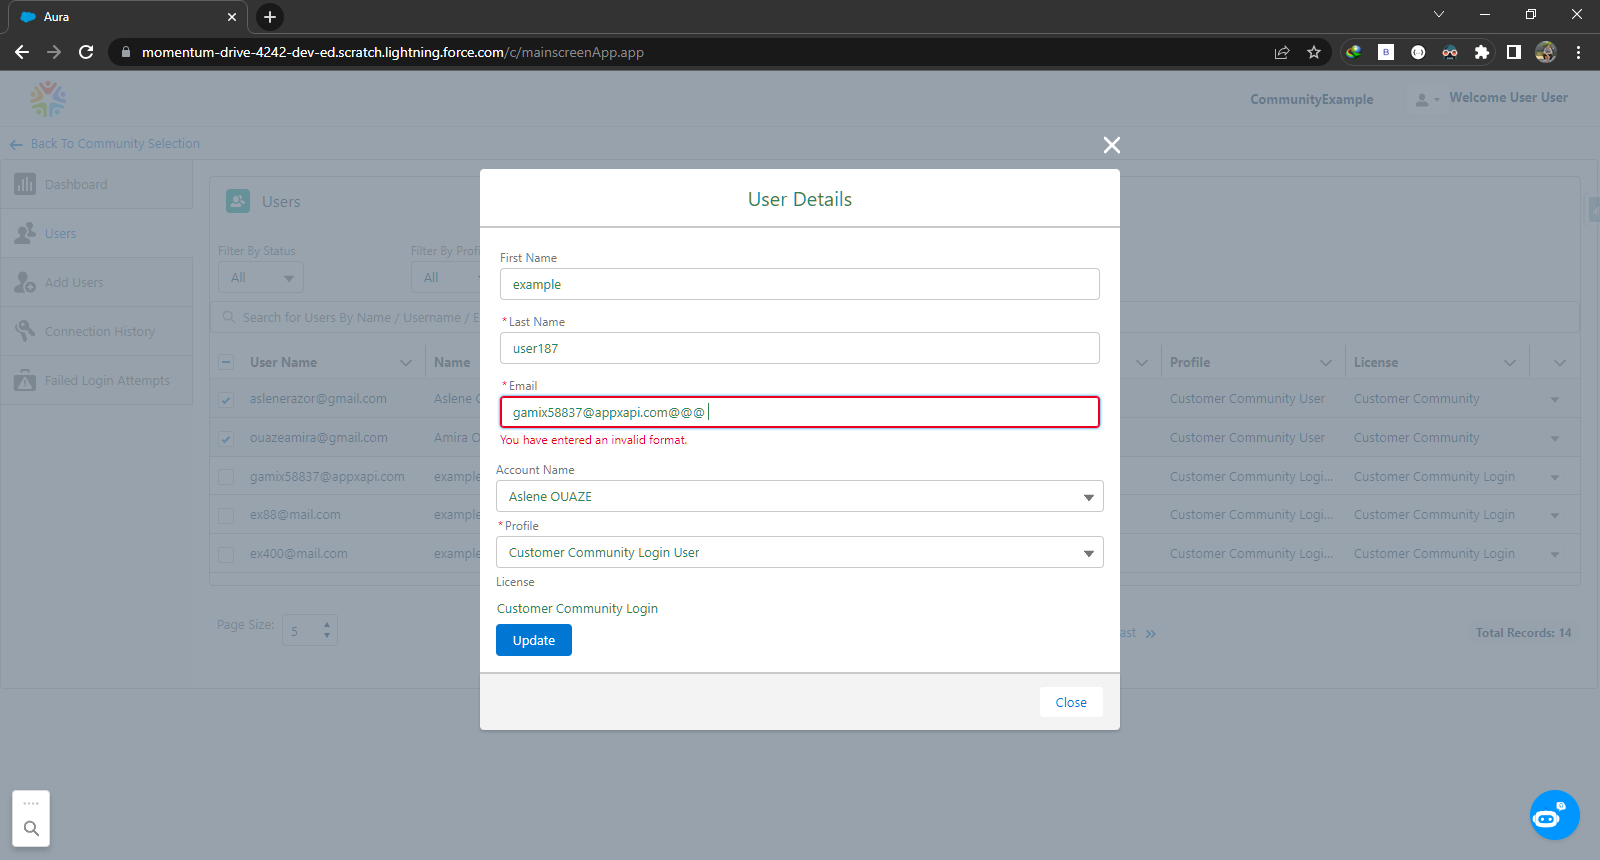
\includegraphics[scale=0.4]{userlist2.png}
    \caption{User details interface}
\end{figure}

\subsection{Add users}
The following figure represents the add users form interface where the user can add one or multiple users using the displayed form fields. The user can fill the initial given form and press the "submit all displayed forms" button where the system will prompt any error message if it exists or the success of the operation otherwise. The user is also able to clone the previously filled form, add a new empty one or delete the latest one using the given buttons.
\begin{figure}[H]%
    \center   
    
    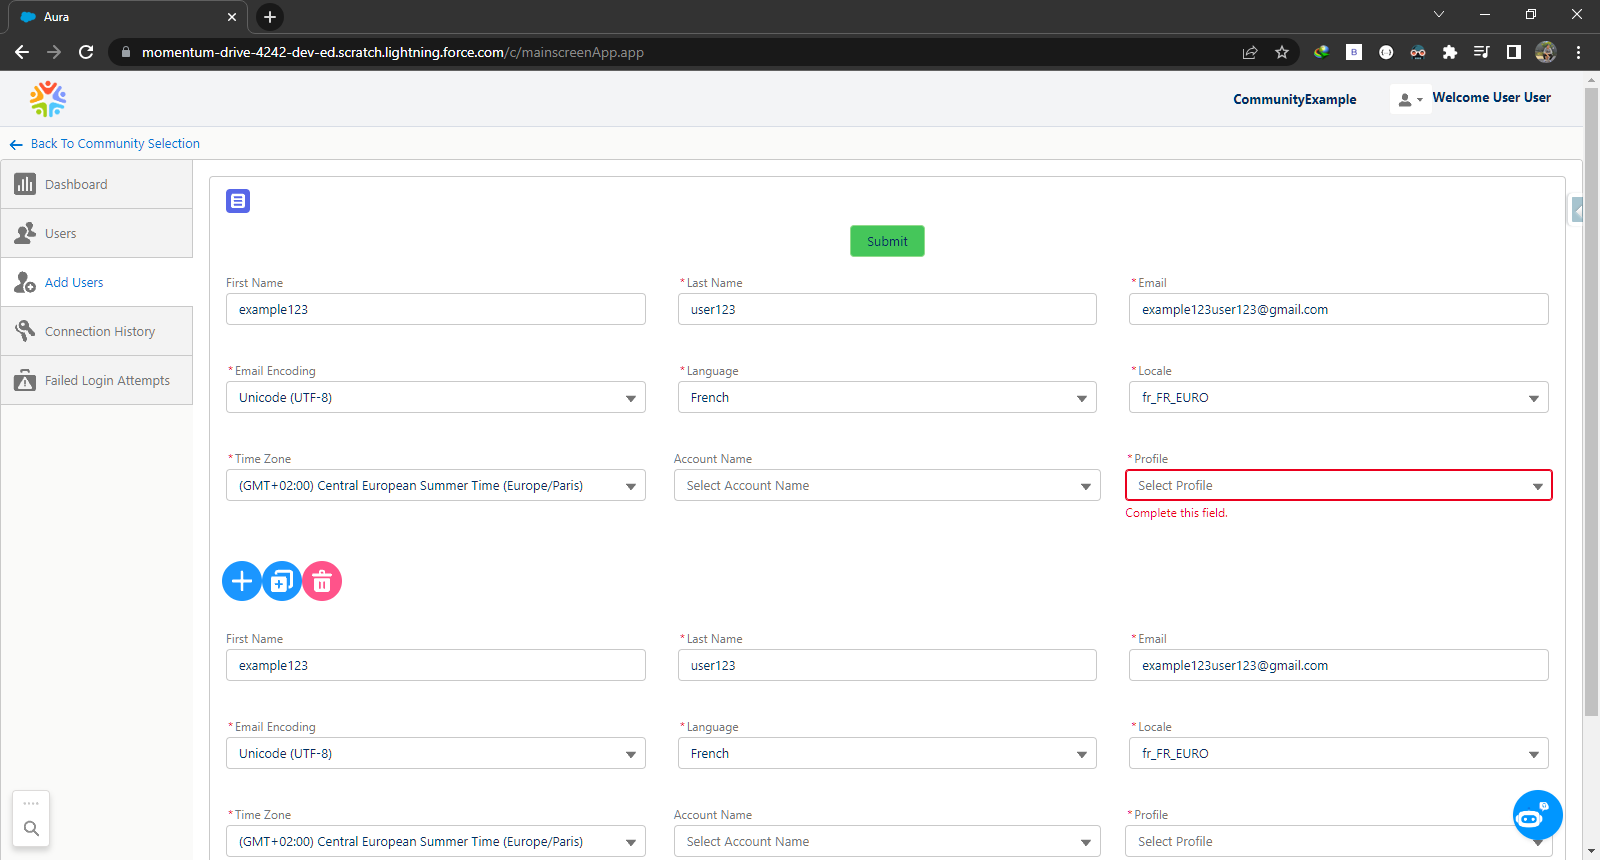
\includegraphics[scale=0.4]{useradd.png}
    \caption{Add users interface}
\end{figure}
\subsection{Connection history}
The following figure represents the connection history interface that shows the number of logins for each user based on the given "from" and "to" dates and time or the time range filter where the user can interact with both of these filters to change the displayed chart.  
\begin{figure}[H]%
    \center   
    
    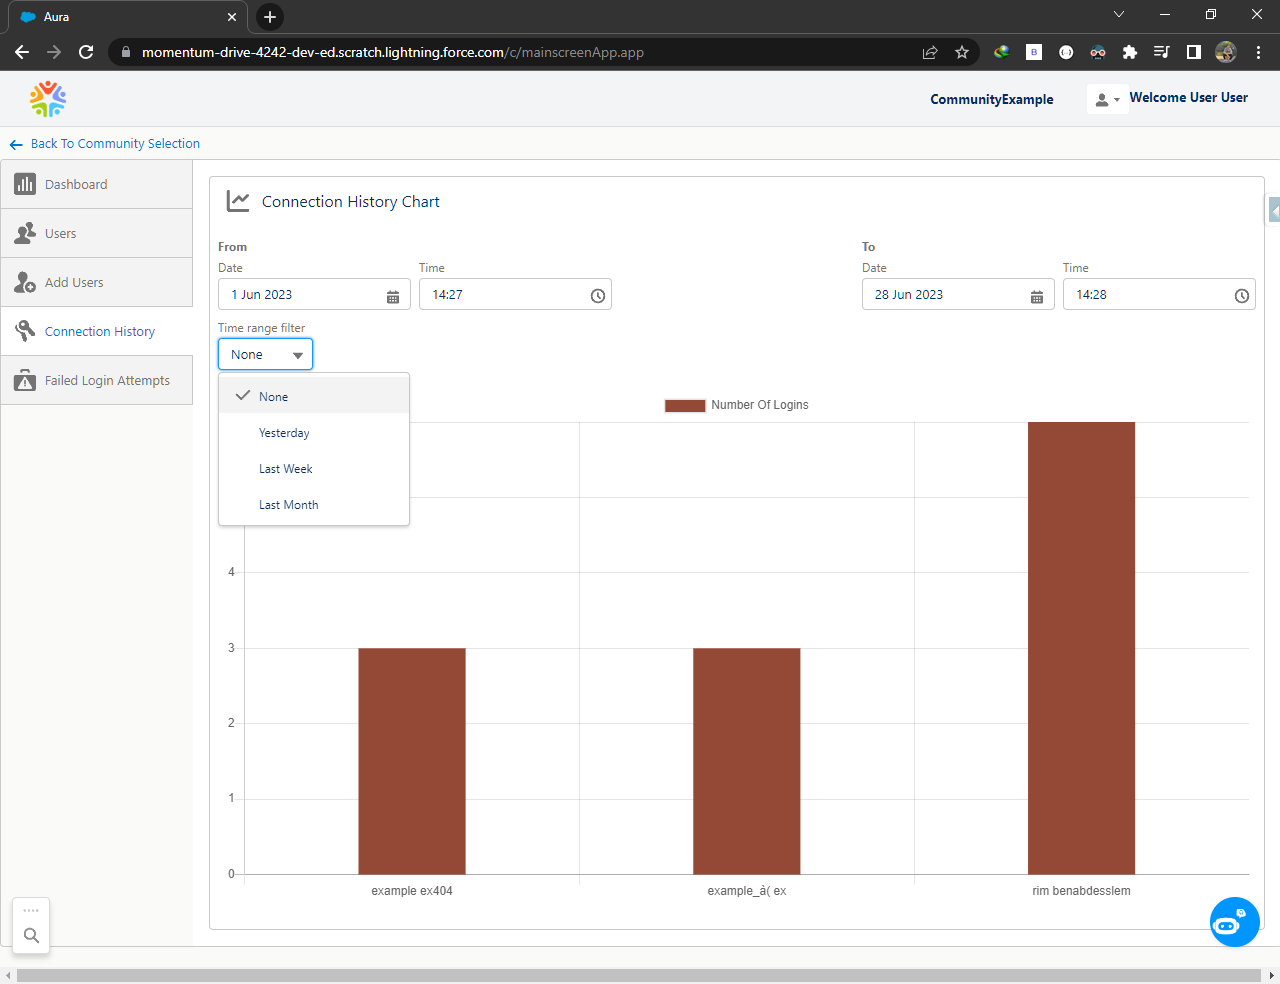
\includegraphics[scale=0.5]{history1.png}
    \caption{Connection history interface (chart)}
\end{figure}
The user may also click one of the displayed bars on the displayed chart to access brief details about the concerned user and update his Salesforce user license as shown in the following figure.
\begin{figure}[H]%
    \center   
    
    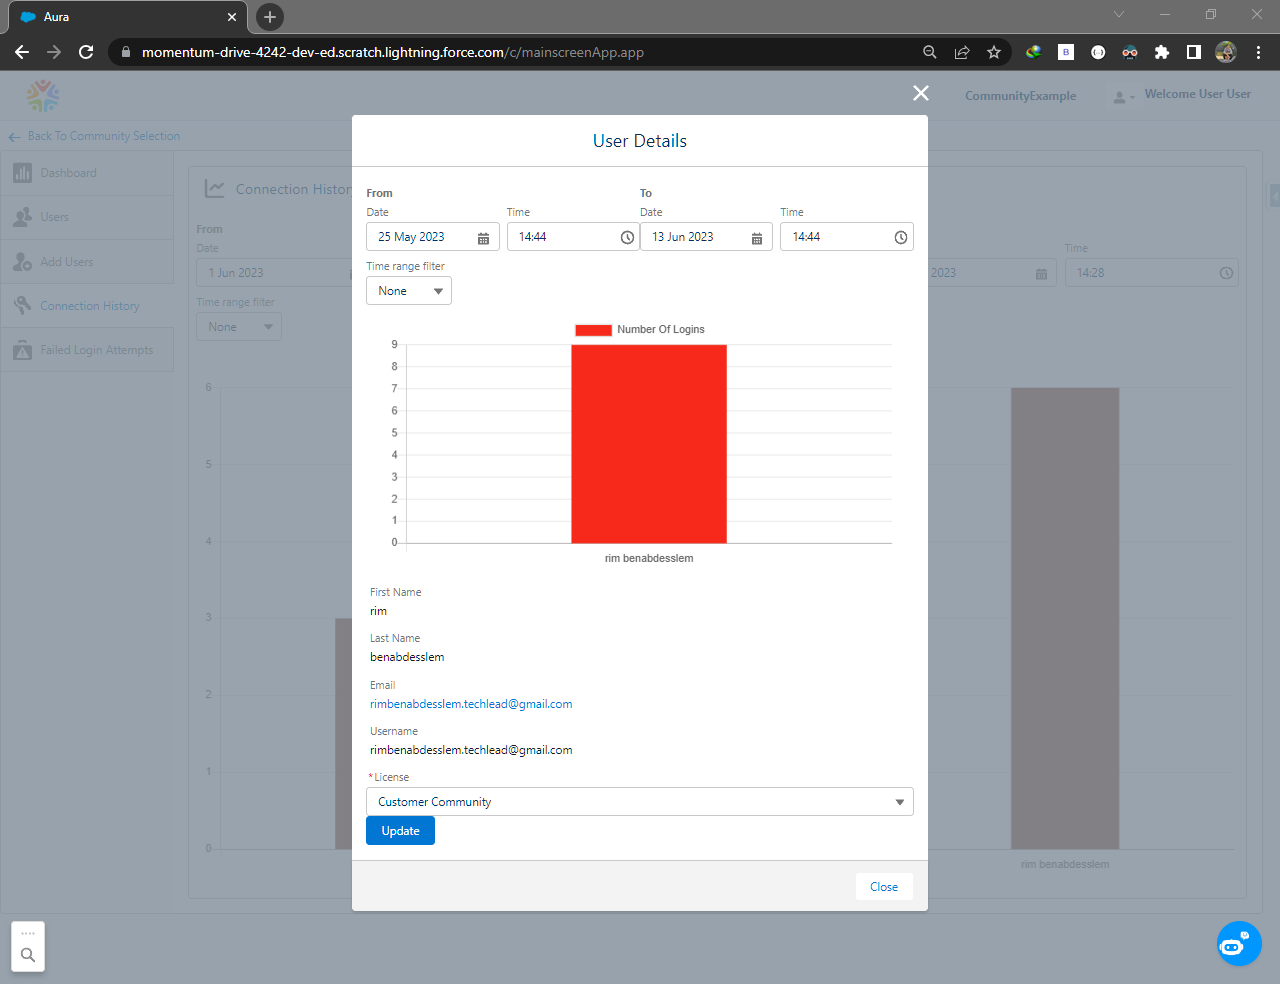
\includegraphics[scale=0.5]{history2.png}
    \caption{Connection history interface (user details)}
\end{figure}
\subsection{Failed login attempts}
The following figure represents the community members' failed login attempts list where the user can navigate through his community login events using given pagination options. He may also filter displayed events by status (invalid password, no community access etc) using the given combo box or search for a specific event using concerned user's Salesforce user name or full name using the provided search bar, he may also filter displayed results by date and time using the provided "from" and "to" filters.\\
The user can also choose to show more details about a specific login event or send a security warning email to the concerned user using the given action menu.

\begin{figure}[H]%
    \center   
    
    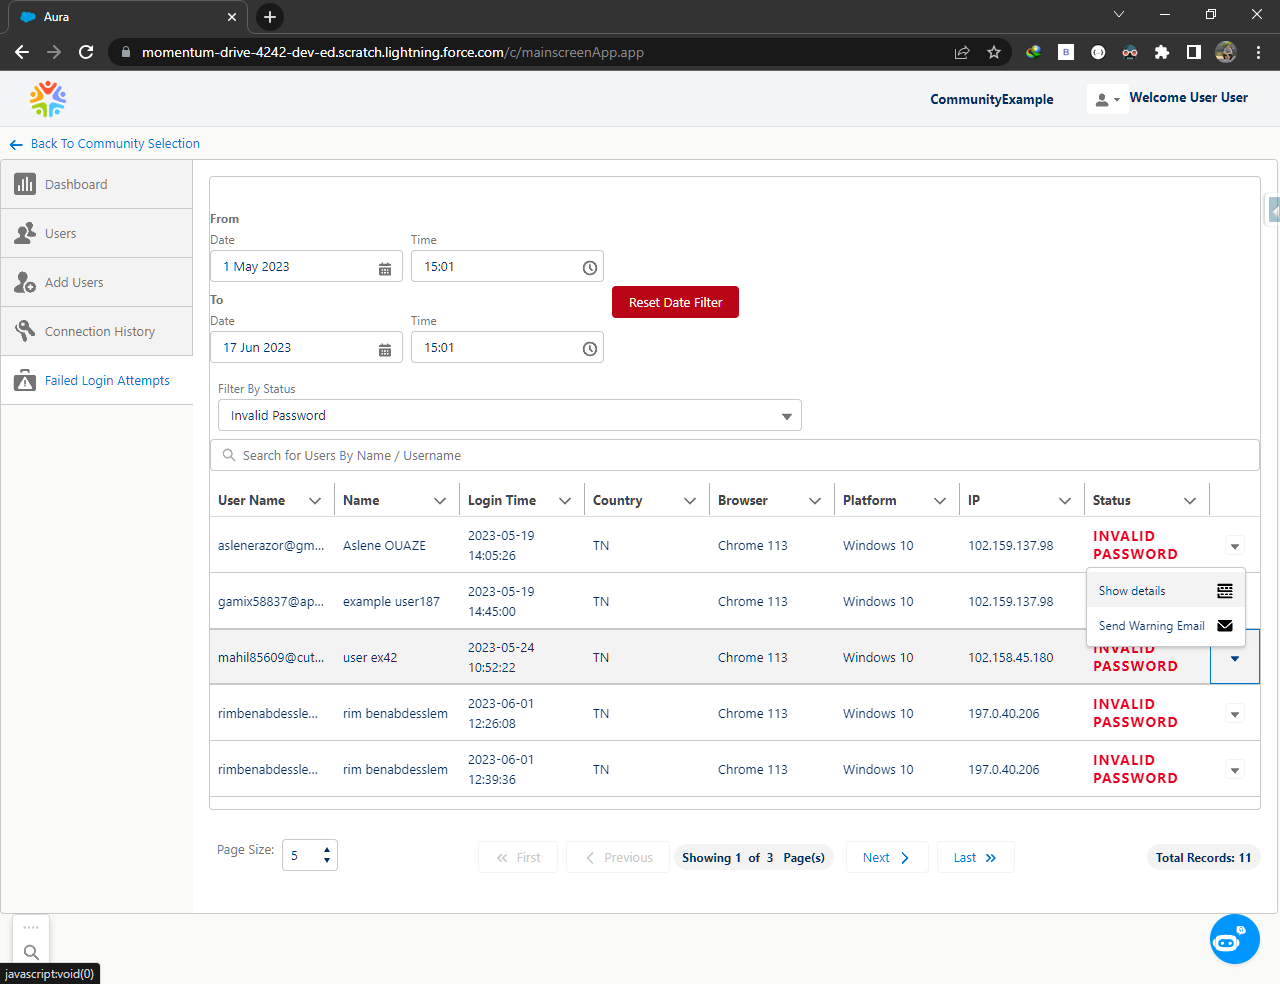
\includegraphics[scale=0.5]{loginattempts1.png}
    \caption{Failed login attempts interface (event list)}
\end{figure}
The following figure represents the selected login event's details interface where the user can navigate the map displaying the event's location in addition to consulting further details about it.
 \begin{figure}[H]%
    \center   
    
    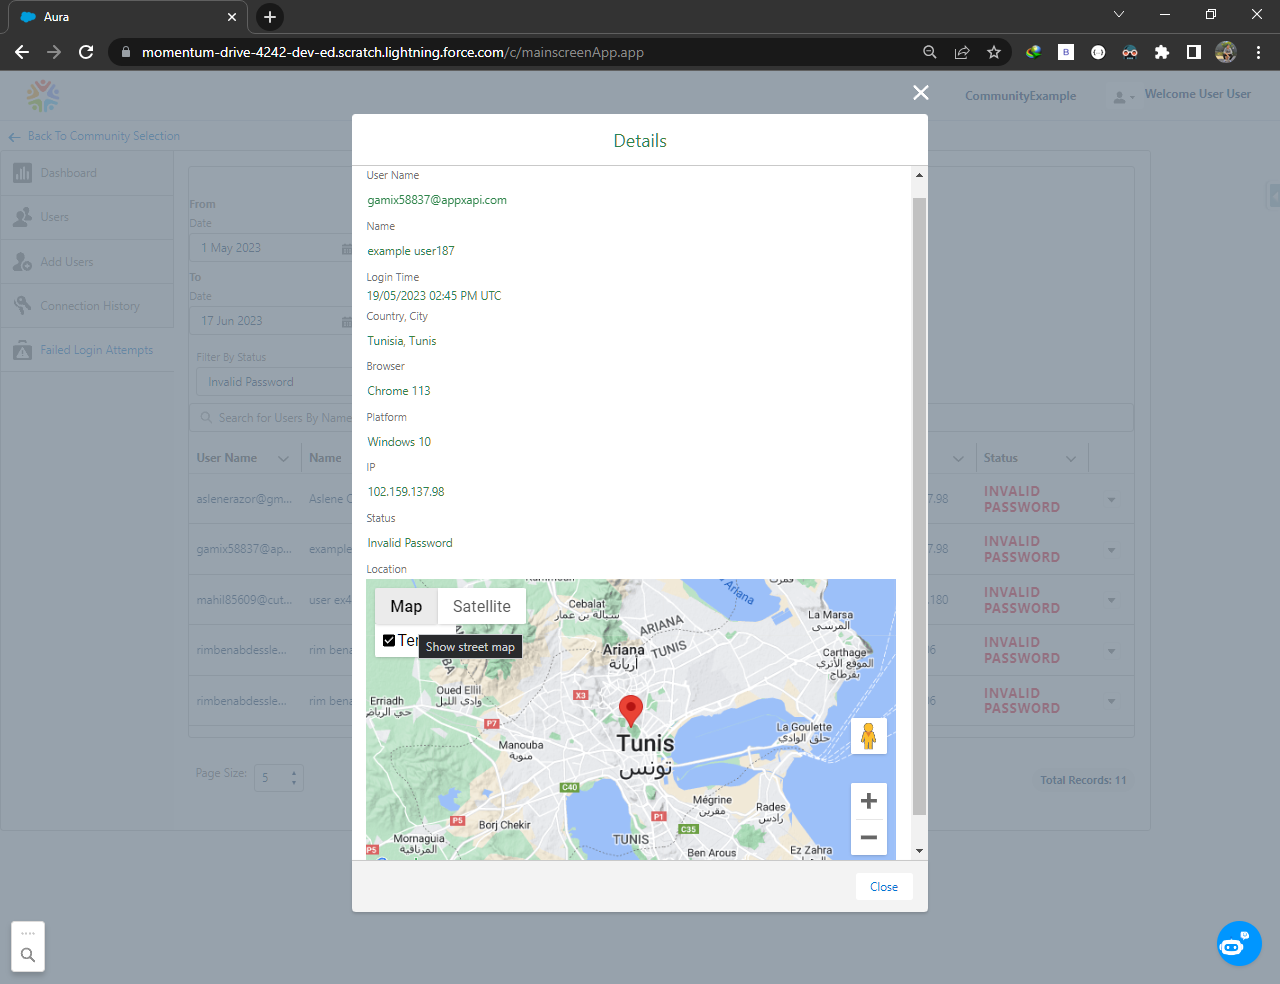
\includegraphics[scale=0.5]{loginattempts2.png}
    \caption{Failed login attempts interface (event details)}
\end{figure}
\subsection{Chatbot}
The following figure represents the Chatbot interface which is accessible from anywhere in the main screen of our application using the floating Chatbot button. In this interface the user may choose one of the predefined questions or type his own question, upon submitting the question the answer will be displayed on screen where the user may choose to give positive or negative feedback to the developers for future improvements.

\begin{figure}[H]%
    \center   
    
    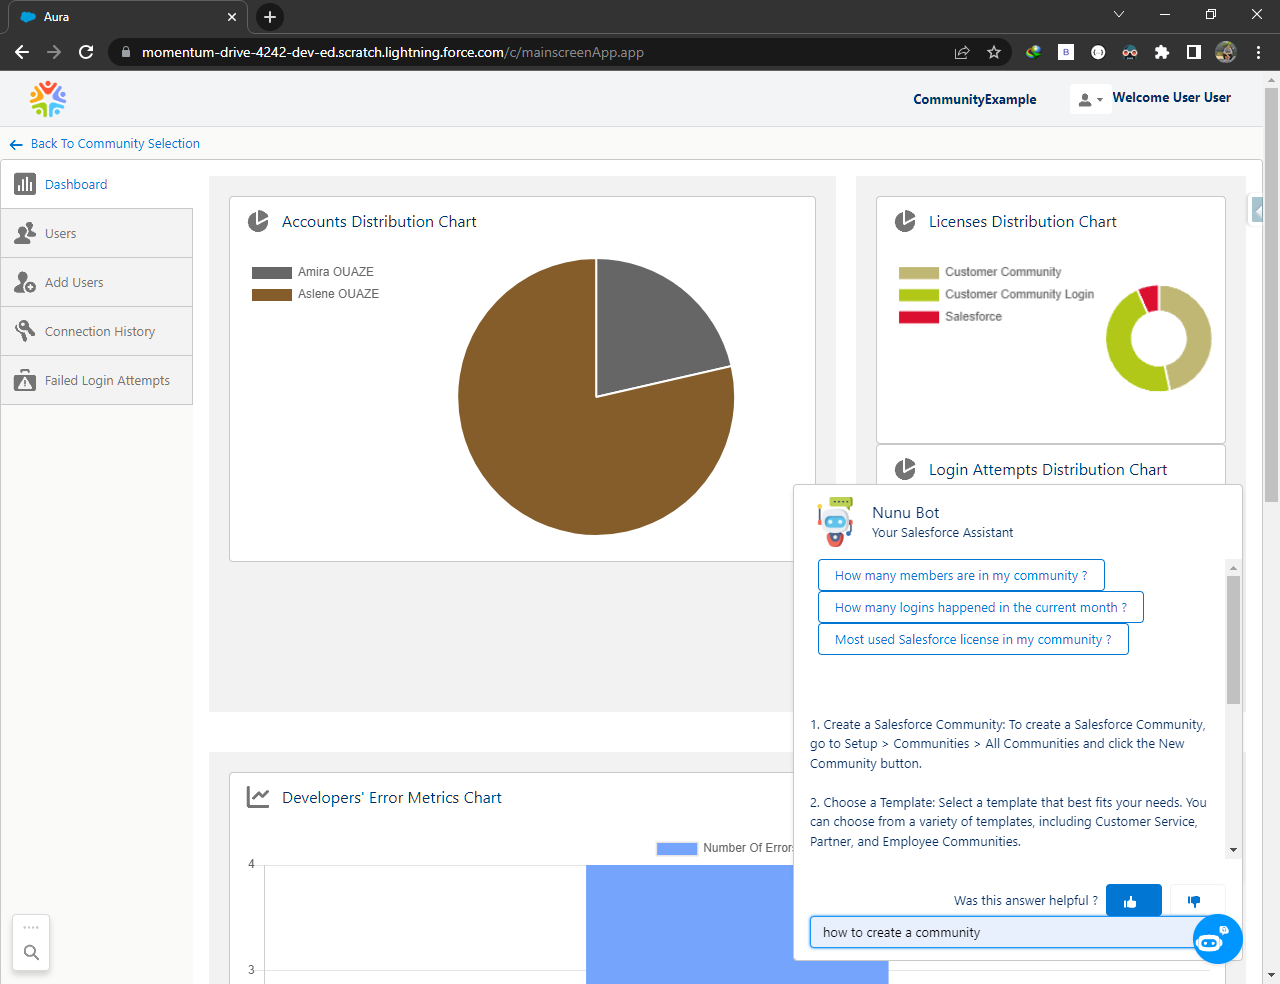
\includegraphics[scale=0.5]{chatbot.png}
    \caption{Chatbot interface}
\end{figure}
\section*{Conclusion}
In this chapter, we presented the technical specification of our
application through the introduction of hardware and software environments. Ultimately,
we have described the features of our application,
illustrated by screenshots of its user interfaces.
We end our report with the general conclusion and the different
prospects.
    \cleardoublepage%
    

    % \chapter{Specification of needs}
\section*{Introduction}
In this chapter, we will identify the actors, then we will specify the functional and non-functional needs that the proposed solution must meet. Finally, we present the use case diagrams explaining our application's main functionalities.
\section{Identification of actors}
An actor represents an external entity that interacts directly with the
system. It can be either a human person or a system. We distinguish
two types of actors, the main actor, and a secondary actor. Indeed,
a principal actor obtains an observable result of the system while a
secondary actor is asked for additional information.\\
\subsection*{Main actors}
\textbf{Community Manager}\\
The community manager is the first main user of our application who should be able to :
\begin{itemize}
\item[•] Choose the community that he has the right to access and manage.
\item[•] Consult users of a specific community inside a well-organized table with pagination options.
\item[•] Filter said users by name, user-name, Salesforce account name, status (active or not active), and Salesforce profile.
\item[•] Consult and update the details of each user.
\item[•] Activate users within a specific community.
\item[•] Deactivate users within a specific community.
\item[•] Send a "Welcome to community" email to a specific active user.
\item[•] Send a "Reset password" email to a specific active user.
\item[•] Add one or multiple users at once to a specific community.
\end{itemize}
In case when the community manager has a Salesforce role he will be also able to :
\begin{itemize}
\item[•] Add one or multiple users at once to a specific community.
\end{itemize}
\textbf{Salesforce Administrator}\\
The Salesforce administrator is the second main user of our application who should be able to :
\begin{itemize}
\item[•] Perform all the actions, mentioned above, that the community manager can.
\item[•] Consult a bar chart that shows the number of logins of each user within the selected community.
\item[•] Filter chart results by the period between two specific dates.
\item[•] Consult details about each user displayed in the chart.
\item[•] Update the Salesforce user license for each user displayed in the chart.
\item[•] Consult users failed login attempts to a specific community inside a well-organized table with pagination options.
\item[•] Filter said login attempts by name, user-name, status( Invalid password, No community access, etc... ) and event date and time.
\item[•] Consult detailed information about each login attempt.
\item[•] Send a security warning email to the account owner about the login attempt event.
\item[•] Access a Chatbot that provides information about the selected community or the Salesforce organization.


\end{itemize}
\subsection*{Secondary actors}
\textbf{Salesforce System}\\
This actor is the system, previously developed and deployed in a cloud server by the Salesforce organization, interactable through our application, and it's responsible for :
\begin{itemize}
\item[•] Sending an automatic "Welcome to community" email upon adding a new member to the community by our application user.  
\item[•] Sending an automatic "Welcome to community" email upon activating a previously deactivated user by our application user.
\item[•] Generating reset password URL upon sending a "Reset password" email to a community member by our application user.
\item[•] Tracking users' successful and failed login attempts and saving them to the organization database.

\end{itemize}
\section{Functional Needs}
Functional needs are expressed by the user of the application
which makes it possible to identify the functionalities of this application.\\
In our
case, the functional needs are:
\begin{itemize}
\item Choice of the community:\\
Select the community to which we will manage the users.

\item Manage users:\\
The system must allow users to be managed with the functionalities of activation,
deactivation, modification, and consultation of the list of users via a data table.
Creation of different filters that allow us to facilitate the navigation of the list of users.

\item Manage connection history:\\
Create a chart that shows the number of user connections per day, week, year, or
according to a well-determined date. This allows the administrator to modify the user’s license.


\item Offer a synthetic dashboard:\\
Allowing the system administrator / the community manager to visualize the KPIs (Key Performance Indicators) of his organization/community.


\end{itemize}
\section{Non-functional Needs}
Non-functional requirements represent the characteristics of the system.
They relate to the constraints to be taken into consideration to set up
an adequate solution.\\
For our application, the non-functional requirements are:
\begin{itemize}
\item Security:\\
Access to information is only possible after verification of privileges and access rights,
for example Authentication, Redirections.

\item Ergonomics and user-friendliness:\\
The application will provide a user-friendly and easy-to-use interface that does not
require any prerequisites, so it can be used by all types of users (even non-computer specialists).

\item Extensibility and maintainability:\\
The architecture of the application will allow the evolution and maintenance (addition
or deletion or update) at the level of its various modules in a flexible manner.

\item Performance:\\
The application must be efficient, i.e. the system must react within a period that does
not exceed 5 seconds, whatever the action of the application.

\item Availability:\\
The application will be available on 24/24 and 7/7 except during maintenance.

\end{itemize}
\section{Use case diagrams}
In this section, we will highlight the system's functionalities to be
from the functional needs mentioned above based on the UML(Unified Modeling Language) diagrams which group together all the system's use cases.
\subsection{Global use case diagram}
The following figure illustrates the global use case diagram of our application
\begin{figure}[H]%
    \center   
    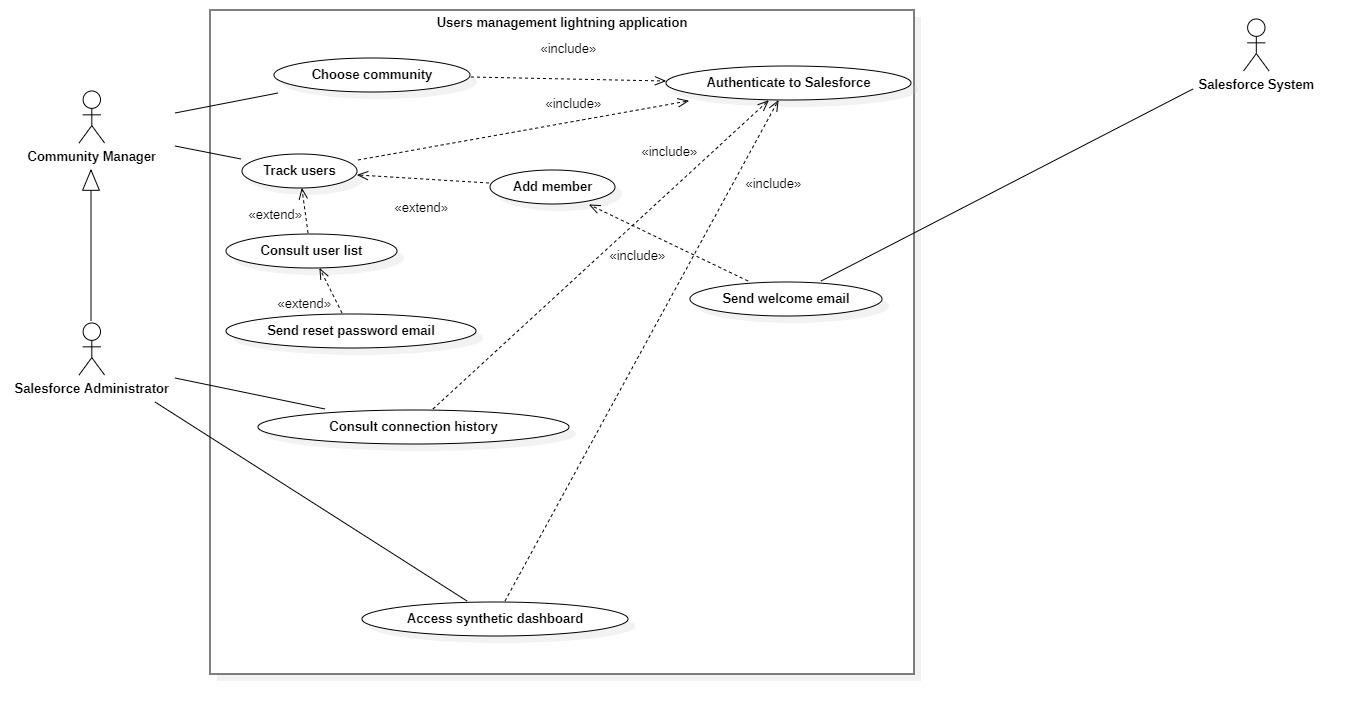
\includegraphics[scale=0.45]{Global UC.jpg}
    \caption{Global use case diagram}
\end{figure}
\subsection{Use case refinement}
In this section, we will detail the main use cases.
\subsubsection{Consult user list use case refinement}
In our application, the community manager and the system administrator can access a data table containing the full list of users within their respective communities.\\
The following figure shows the Consult user list use case diagram.
\begin{figure}[H]%
    \center   
    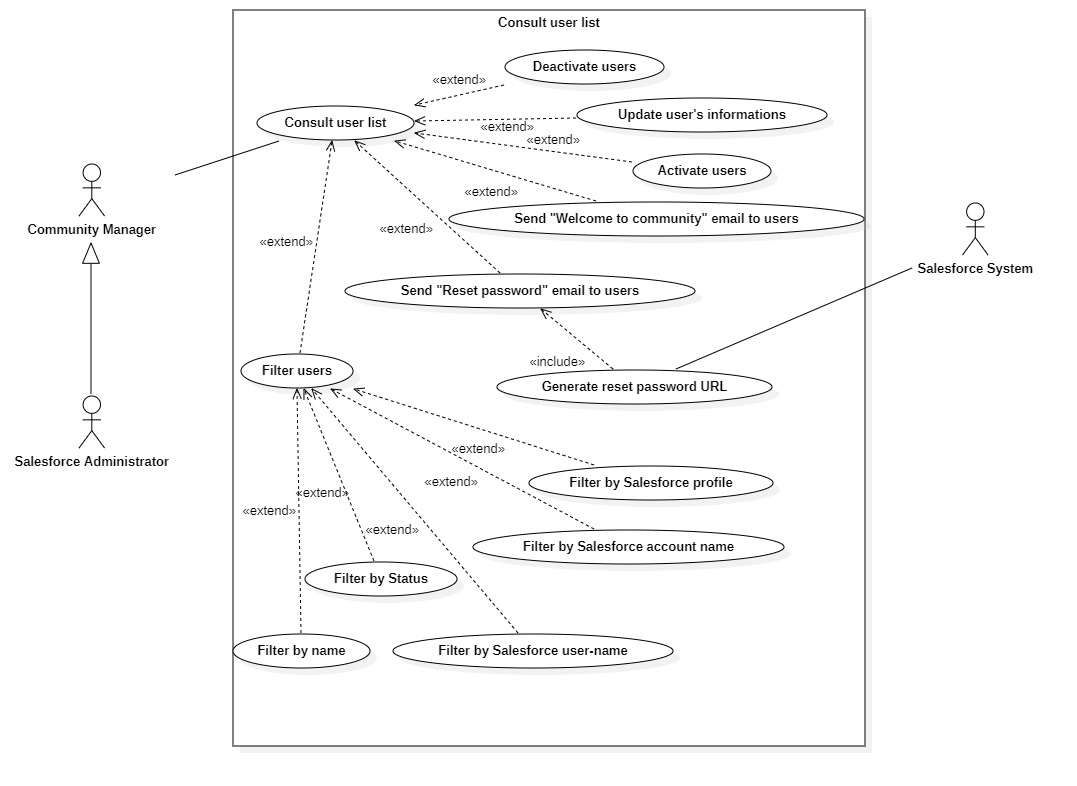
\includegraphics[scale=0.5]{Consult users list UC.jpg}
    \caption{Consult user list use case diagram}
\end{figure}
The following table details the tasks to be performed by the user to manage the user list.

\begin{table}[H]
\footnotesize% or \small or \scriptsize
\begin{tabular}{|ll|}
\hline
\multicolumn{2}{|c|}{\textbf{Summary}}                                                                                                                                                                                                                                                                                                                                                                                                                                                                                                                                                                                                                                                                                                                                                         \\ \hline
\multicolumn{1}{|l|}{Title}                      & Consult user list                                                                                                                                                                                                                                                                                                                                                                                                                                                                                                                                                                                                                                                                                                                           \\ \hline
\multicolumn{1}{|l|}{Objectif}                   & \begin{tabular}[c]{@{}l@{}}Allowing the community manager or the system administrator\\ to manage his community members\end{tabular}                                                                                                                                                                                                                                                                                                                                                                                                                                                                                                                                                                                                        \\ \hline
\multicolumn{1}{|l|}{Actors}                     & Community manager, System administrator                                                                                                                                                                                                                                                                                                                                                                                                                                                                                                                                                                                                                                                                                                     \\ \hline
\multicolumn{2}{|c|}{\textbf{Description of sequences}}                                                                                                                                                                                                                                                                                                                                                                                                                                                                                                                                                                                                                                                                                                                                        \\ \hline
\multicolumn{1}{|l|}{Pre-condition}              & \begin{tabular}[c]{@{}l@{}}- User should be authenticated to Salesforce\\ - User should be the owner of at least one community\end{tabular}                                                                                                                                                                                                                                                                                                                                                                                                                                                                                                                                                                                                 \\ \hline
\multicolumn{1}{|l|}{Post-condition}             & - Community members are well organized                                                                                                                                                                                                                                                                                                                                                                                                                                                                                                                                                                                                                                                                                                      \\ \hline
\multicolumn{1}{|l|}{Normal scenario}            & \begin{tabular}[c]{@{}l@{}}1. User accesses the user list interface\\ 2. User selects one or many community members\\ 3. User clicks the "activate/deactivate" button for selected members\\ 4. The system prompts the success of the operation\\ 5. The user clicks the "Send welcome email" button\\ for the selected members\\ 6. The system prompts the success of the operation\\ 7. The user clicks the "Send reset password" button\\ for the selected members\\ 8. The system prompts the success of the operation\\ 9. The user clicks the "show details" button for one member\\ 10. The member information interface pops up \\ 11. User updates the selected member information and complies\\ 12. System prompts the success of the operation\end{tabular} \\ \hline
\multicolumn{1}{|l|}{Alternative scenario}       & \begin{tabular}[c]{@{}l@{}}1. License limit exceeded when activating members: The system\\ sends an error message\\ 2. Sending a welcome email to a deactivated member: The system\\ sends an error message\\ 3. Changing member username to an existing one: The system\\ sends an error message\end{tabular}                                                                                                                                                                                                                                                                                                                                                                                                                              \\ \hline
\multicolumn{1}{|l|}{Non-functional constraints} & \begin{tabular}[c]{@{}l@{}}1. The interface must be ergonomic\\ 2. Error messages should be understandable and clear\end{tabular}                                                                                                                                                                                                                                                                                                                                                                                                                                                                                                                                                                                                           \\ \hline
\end{tabular}
\captionsetup{skip=5pt} % Adjust the skip value as per your needs
\caption{Consult user list use case}

\end{table}
\pagebreak
\subsubsection{Add members use case refinement}
In our application, the community manager and the system administrator can add one or multiple members at once to their respective communities.\\

The following table details the tasks to be performed by the user to add members to his community.

\begin{table}[H]
\begin{tabular}{|ll|}
\hline
\multicolumn{2}{|c|}{\textbf{Summary}}                                                                                                                                                                                                                                                                                                                                                                                                                                                                                                                                                                                                                                                                                      \\ \hline
\multicolumn{1}{|l|}{Title}                      & Add members                                                                                                                                                                                                                                                                                                                                                                                                                                                                                                                                                                                                                                                              \\ \hline
\multicolumn{1}{|l|}{Objectif}                   & \begin{tabular}[c]{@{}l@{}}Allowing the community manager or the system administrator to \\ add one or multiple members at once to his community\end{tabular}                                                                                                                                                                                                                                                                                                                                                                                                                                                                                                            \\ \hline
\multicolumn{1}{|l|}{Actors}                     & Community manager, System administrator                                                                                                                                                                                                                                                                                                                                                                                                                                                                                                                                                                                                                                  \\ \hline
\multicolumn{2}{|c|}{\textbf{Description of sequences}}                                                                                                                                                                                                                                                                                                                                                                                                                                                                                                                                                                                                                                                                     \\ \hline
\multicolumn{1}{|l|}{Pre-condition}              & \begin{tabular}[c]{@{}l@{}}- User should be authenticated to Salesforce\\ - User should be the owner of at least one community\\ - User should have a Salesforce role\end{tabular}                                                                                                                                                                                                                                                                                                                                                                                                                                                                                       \\ \hline
\multicolumn{1}{|l|}{Post-condition}             & - New member(s) are added to the owner's community                                                                                                                                                                                                                                                                                                                                                                                                                                                                                                                                                                                                                       \\ \hline
\multicolumn{1}{|l|}{Normal scenario}            & \begin{tabular}[c]{@{}l@{}}1. User accesses the add members interface\\ 2. The user fills the displayed form with information about the new member\\ 3. The user clicks the " add another member" button\\ 4. A new empty form, identical to the previous one, is displayed\\ 5. The user fills the new form with information about the next new member\\ 6. The user clicks the "clone member" button\\ 7. A new form containing the same values as the previous form is displayed\\ 8. The user clicks the "delete form" button\\ 9. The selected form is deleted from the screen\\ 10. The user clicks the "submit" button \\ 11. System prompts the success of the operations\end{tabular} \\ \hline
\multicolumn{1}{|l|}{Alternative scenario}       & \begin{tabular}[c]{@{}l@{}}1. Empty fields: The system sends an error message:\\ You must complete all the required fields\\ 2. The email entered is not valid: The system sends an error message\\ describing the validation conditions for this field\\ 3. Duplicate Salesforce user-name: The system sends an error message\end{tabular}                                                                                                                                                                                                                                                                                                                              \\ \hline
\multicolumn{1}{|l|}{Non-functional constraints} & \begin{tabular}[c]{@{}l@{}}1. The interface must be ergonomic\\ 2. Error messages should be understandable and clear\end{tabular}                                                                                                                                                                                                                                                                                                                                                                                                                                                                                                                                        \\ \hline
\end{tabular}
\captionsetup{skip=5pt} % Adjust the skip value as per your needs
\caption{Add members use case}

\end{table}
\subsubsection{Consult synthetic dashboard use case refinement}
In our application, the community manager and the system administrator can access a dashboard containing features that helps them to manage their respective communities.\\
The following figure shows the Consult synthetic use case diagram.
\begin{figure}[H]%
    \center   
    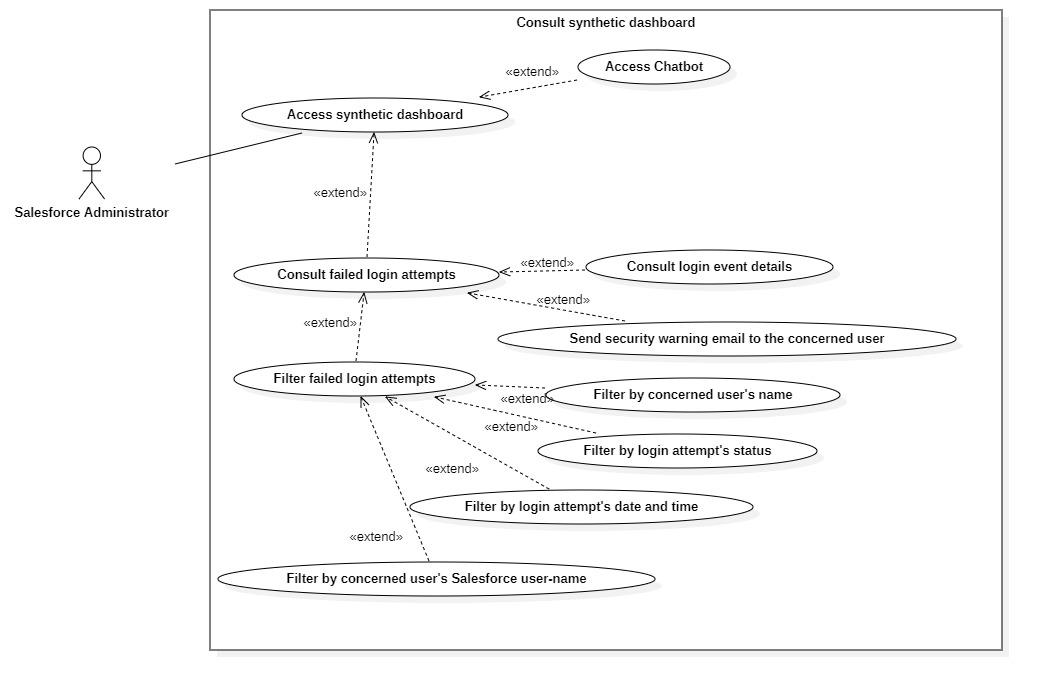
\includegraphics[scale=0.5]{Consult synthetic dashboard UC.jpg}
    \caption{Consult synthetic dashboard use case diagram}
\end{figure}

The following table details the tasks to be performed by the customer to consult the synthetic dashboard
in our application.
\begin{table}[H]
\begin{tabular}{|ll|}
\hline
\multicolumn{2}{|c|}{\textbf{Summary}}                                                                                                                                                                                       \\ \hline
\multicolumn{1}{|l|}{Title}                      & Consult synthetic dashboard                                                                                                                                               \\ \hline
\multicolumn{1}{|l|}{Objectif}                   & \begin{tabular}[c]{@{}l@{}}Allowing the system administrator\\ to access extra features that helps him to manage his communities\end{tabular} \\ \hline
\multicolumn{1}{|l|}{Actors}                     & System administrator                                                                                                                                   \\ \hline
\multicolumn{2}{|c|}{\textbf{Description of sequences}}                                                                                                                                                                      \\ \hline
\multicolumn{1}{|l|}{Pre-condition}              & \begin{tabular}[c]{@{}l@{}}- User should be authenticated to Salesforce\\ - User should be the owner of at least one community\end{tabular}                               \\ \hline
\multicolumn{1}{|l|}{Post-condition}             & \begin{tabular}[c]{@{}l@{}}- System administrator is well informed\\ about his respective community.\end{tabular}                                \\ \hline
\multicolumn{1}{|l|}{Normal scenario}            & \begin{tabular}[c]{@{}l@{}}1. User accesses the dashboard interface\\ 2. User selects the wanted feature \\ 3. The selected feature interface pops up.\end{tabular}       \\ \hline
\multicolumn{1}{|l|}{Alternative scenario}       &                                                                                                                                                                           \\ \hline
\multicolumn{1}{|l|}{Non-functional constraints} & 1. The interface must be ergonomic                                                                                                                                        \\ \hline
\end{tabular}
\caption{Consult synthetic dashboard use case}
\end{table}


The following table details the tasks to be performed by the customer to consult the failed login attempts
in our application.
\begin{table}[H]
\begin{tabular}{|ll|}
\hline
\multicolumn{2}{|c|}{\textbf{Summary}}                                                                                                                                                                                                                                                                                                                                                                                                                                                                                                                           \\ \hline
\multicolumn{1}{|l|}{Title}                      & Consult failed login attempts                                                                                                                                                                                                                                                                                                                                                                                                                                                                                 \\ \hline
\multicolumn{1}{|l|}{Objectif}                   & \begin{tabular}[c]{@{}l@{}}Allowing  the system administrator\\ to access failed login attempts and inform concerned users about them\end{tabular}                                                                                                                                                                                                                                                                                                                                                            \\ \hline
\multicolumn{1}{|l|}{Actors}                     & System administrator                                                                                                                                                                                                                                                                                                                                                                                                                                                                                          \\ \hline
\multicolumn{2}{|c|}{\textbf{Description of sequences}}                                                                                                                                                                                                                                                                                                                                                                                                                                                                                                          \\ \hline
\multicolumn{1}{|l|}{Pre-condition}              & \begin{tabular}[c]{@{}l@{}}- User should be authenticated to Salesforce\\ - User should be the owner of at least one community\end{tabular}                                                                                                                                                                                                                                                                                                                                                                   \\ \hline
\multicolumn{1}{|l|}{Post-condition}             & - Users are well-informed about their account security status.                                                                                                                                                                                                                                                                                                                                                                                                                                                \\ \hline
\multicolumn{1}{|l|}{Normal scenario}            & \begin{tabular}[c]{@{}l@{}}1. User accesses the failed login attempts interface\\ 2. The user clicks the "show details" button for a specific login event\\ 3. The "show details" interface for the selected login event pops up\\ 4. The user clicks the "send security warning email" button for\\ the specific login event\\ 5. The system prompts the success of the operation\\ 6. The concerned user receives the warning email, containing details\\ about the failed login attempt, in his email\end{tabular} \\ \hline
\multicolumn{1}{|l|}{Alternative scenario}       & \begin{tabular}[c]{@{}l@{}}1. Server error when sending the warning email: The system\\ sends an error message received from the server\end{tabular}                                                                                                                                                                                                                                                                                                                                                          \\ \hline
\multicolumn{1}{|l|}{Non-functional constraints} & \begin{tabular}[c]{@{}l@{}}1. The interface must be ergonomic\\ 2. Error messages should be understandable and clear\end{tabular}                                                                                                                                                                                                                                                                                                                                                                             \\ \hline
\end{tabular}
\caption{Consult failed login attempts use case}
\end{table}



\subsubsection{Access Chatbot use case refinement}
The following figure illustrates the use case diagram "Access Chatbot"

\begin{figure}[H]%
    \center   
    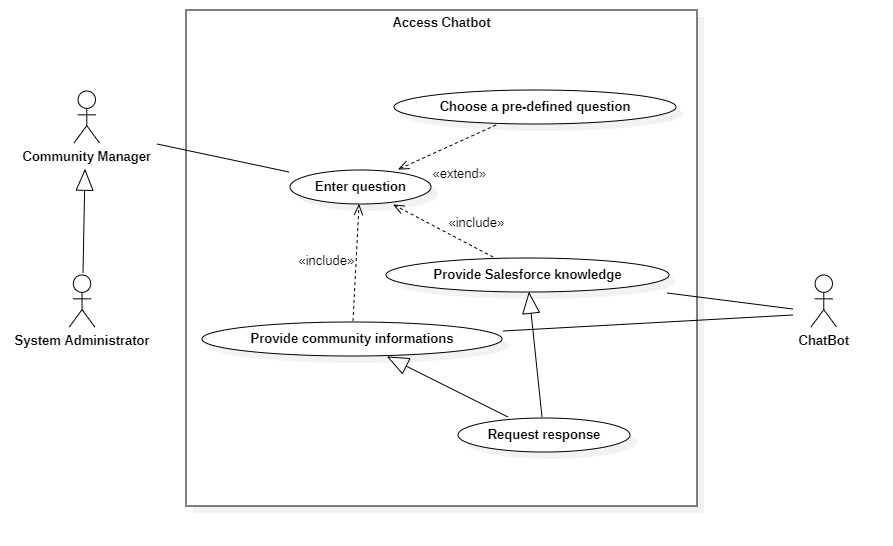
\includegraphics[scale=0.5]{Access Chatbot.jpg}
    \caption{Access Chatbot use case diagram}
\end{figure}

The following table details the tasks to be performed by the customer to Access the Chatbot within our app.
\begin{table}[H]
\begin{tabular}{|ll|}
\hline
\multicolumn{2}{|c|}{\textbf{Summary}}                                                                                                                                                                                                                                                                                                                              \\ \hline
\multicolumn{1}{|l|}{Title}                      & Access Chatbot                                                                                                                                                                                                                                                                                                   \\ \hline
\multicolumn{1}{|l|}{Objectif}                   & \begin{tabular}[c]{@{}l@{}}Trigger a Chatbot that responds to user requests \\ while providing informations about the current community\end{tabular}                                                                                                                                                             \\ \hline
\multicolumn{1}{|l|}{Actors}                     & System administrator, Chatbot                                                                                                                                                                                                                                                                                    \\ \hline
\multicolumn{2}{|c|}{\textbf{Description of sequences}}                                                                                                                                                                                                                                                                                                             \\ \hline
\multicolumn{1}{|l|}{Pre-condition}              & \begin{tabular}[c]{@{}l@{}}- User should be authenticated to Salesforce\\ - User should be the owner of at least one community\end{tabular}                                                                                                                                                                      \\ \hline
\multicolumn{1}{|l|}{Post-condition}             & \begin{tabular}[c]{@{}l@{}} - User question is answered\\ and the response is displayed on the screen. \end{tabular}                                                                                                                                                                                                                                             \\ \hline
\multicolumn{1}{|l|}{Normal scenario}            & \begin{tabular}[c]{@{}l@{}}1. User accesses the Chatbot interface\\ 2. User types a question or selects a predefined question.\\ 3. The chatbot is launched upon receipt of a request\\ 4. The chatbot analyzes the request\\5. The chatbot prepares the response\\ 6. The chatbot sends the response\end{tabular} \\ \hline
\multicolumn{1}{|l|}{Alternative scenario}       & 1. An error message is displayed if the question\\ is not recognized by the system.                                                                                                                                                                                                                                 \\ \hline
\multicolumn{1}{|l|}{Non-functional constraints} & \begin{tabular}[c]{@{}l@{}}1. The interface must be ergonomic\\ 2. Error messages should be understandable and clear\\ 3. The ChatBot must always be available.\end{tabular}                                                                                                                                     \\ \hline
\end{tabular}

\caption{Access Chatbot use case}
\end{table}

\pagebreak
\section*{Conclusion}
In this chapter, we have described the specification phases of the
needs of our developed application to identify the different actors
as well as the features and services that our application must provide.\\
We have detailed these features with use case diagrams. The next chapter will be devoted to the conception phase.
    % \cleardoublepage%

    % \chapter{Conception}
\section*{Introduction}
After identifying the functional and non-functional needs and the main functionalities of our application. We begin this part
of the conceptual study by describing the general architecture of our system and
it's detailed internal modeling through class and sequence diagrams.
\section{Global Architecture}
In this section, we will give an overview of the definition of the
the architectural pattern was chosen to model our application and we will
detail the projection of this pattern on our application.

\subsection{Definition of the Model-View-Controller design pattern}
Our chosen architecture of work for this project will be the MVC  architecture since it is recommended by the Salesforce developer’s community.\\
The model-view-controller (MVC) design pattern specifies that an application consists of a data model, presentation information, and control information.\cite{5} \\
The pattern requires that each of these be separated into different objects:
\begin{itemize}
\item \textbf{The model} (for example, the data information) contains only pure application data; it contains no logic describing how to present the data to a user. \cite{5}
\item \textbf{The view} (for example, the presentation information) presents the model's data to the user. The view knows how to access the model's data but does not know what this data means or what the user can do to manipulate it. \cite{5}
\item \textbf{The controller} (for example, the control information) exists between the view and the model. It listens to events triggered by the view (or another external source) and executes the appropriate reaction to these events. In most cases, the reaction is to call a method on the model. Since the view and the model are connected through a notification mechanism, the result of this action is then automatically reflected in the view.\cite{5}
\end{itemize}
Thanks to these principles, the components of the application become easy to
manage, test, modify, and reuse.\\
The following figure explains furthermore the role and the idea behind each component of the MVC pattern:

\begin{figure}[H]%
    \center   
    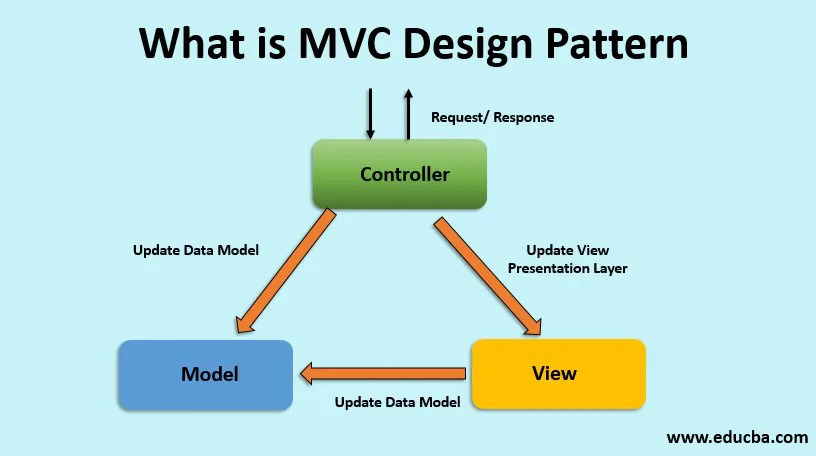
\includegraphics[scale=0.5]{mvc2.jpg}
    \caption{Understanding MVC Design Pattern, Source: \cite{7}}
\end{figure}
\subsection{Application of the "MVC" pattern}
We explain in this paragraph the details of the projection of the pattern
MVC on our app.\\
The following figure represents the class diagram which illustrates the binding
between entities (classes). Indeed, this diagram translates the content of the \textbf{Model} component, and it's based on the schema that is already established within the Salesforce infrastructure.
\begin{figure}[H]%
    \center   
    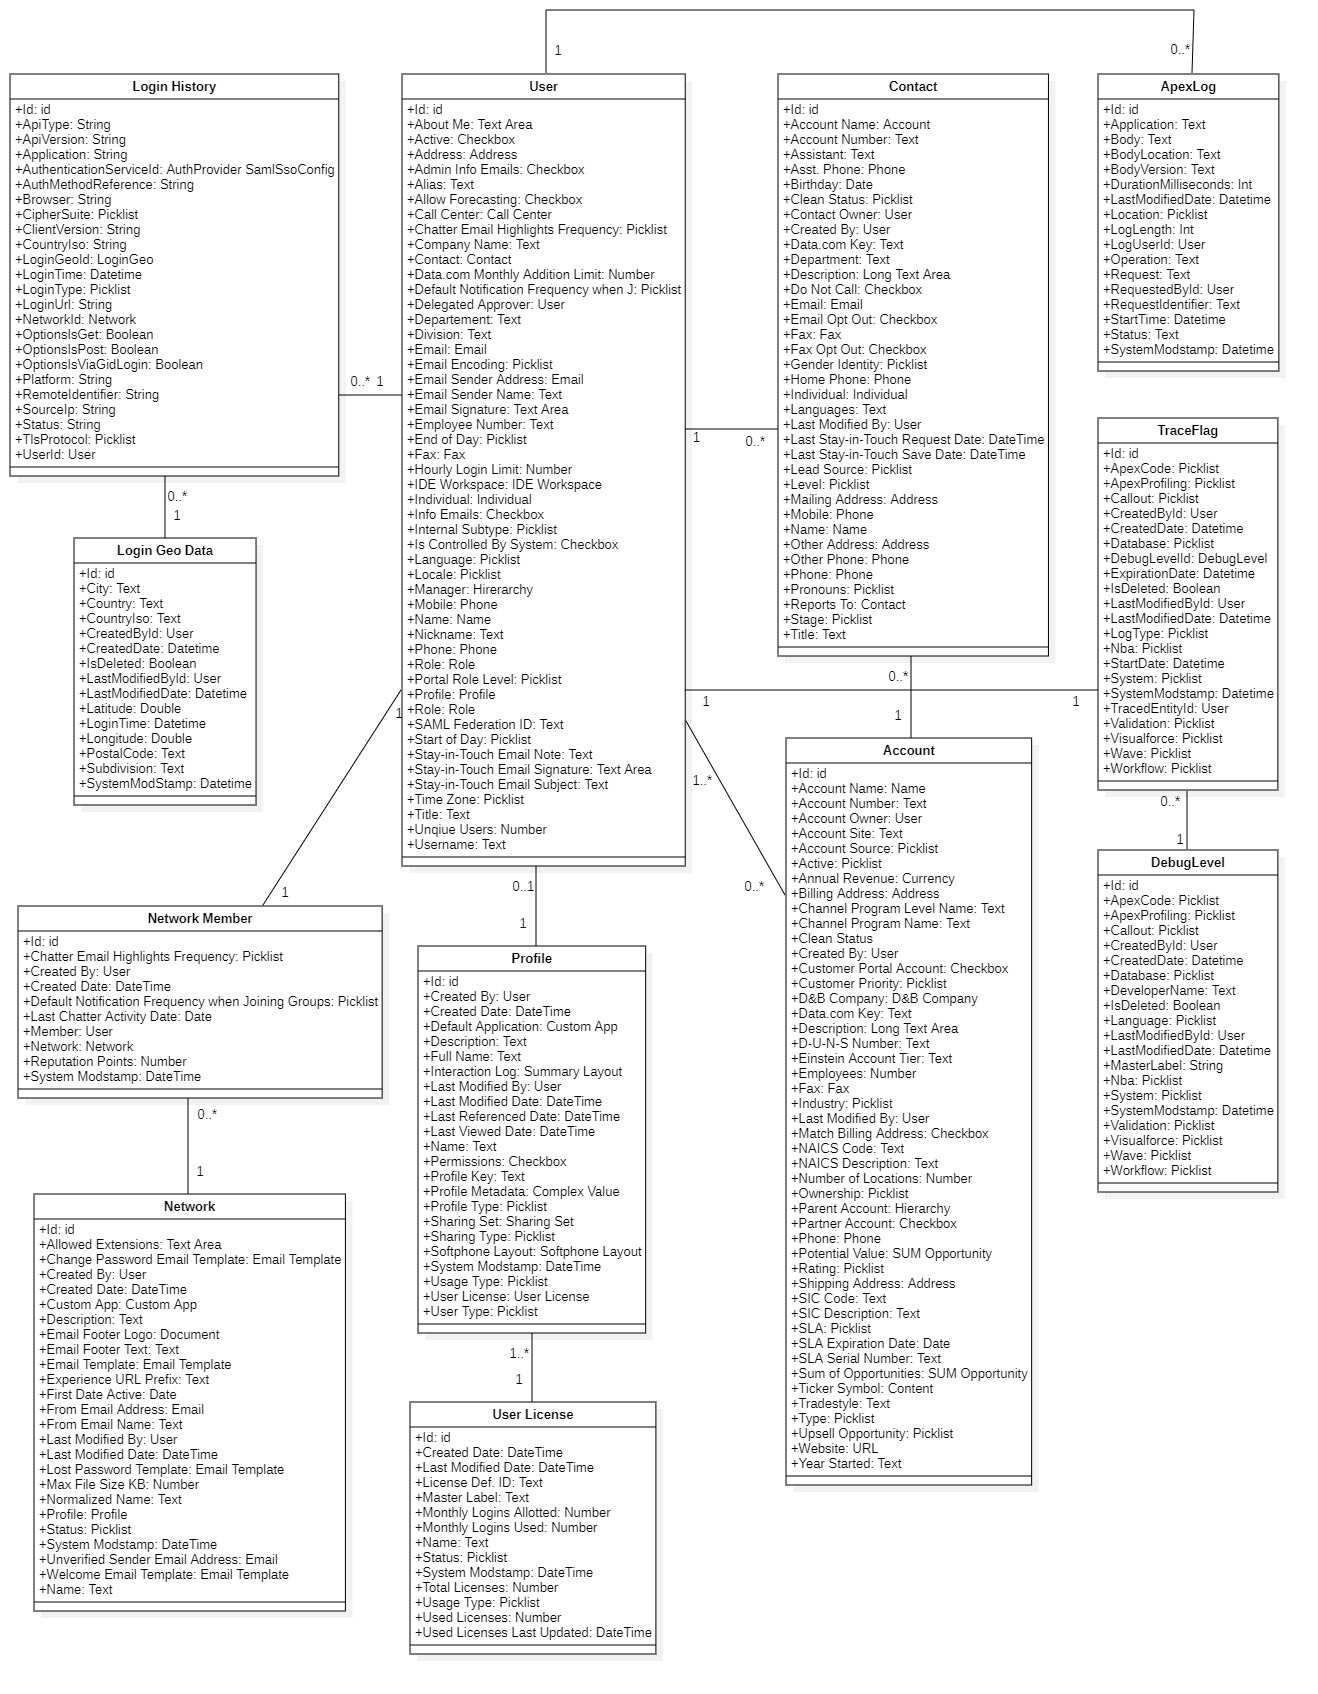
\includegraphics[scale=0.4]{ClassDiagram.jpg}
    \caption{Class diagram representing the "Model" component}
\end{figure}
\newpage
Description of classes representing our Model:
\begin{itemize}
\item \textbf{User:}\\
This class represents our application's Salesforce user, who is the main focus of the administrator and community managers main focus when working within our app. This class's most important attributes in our application are:
\begin{itemize}
\item[•] Id: the unique identification key for the user 
\item[•] Active: determines the status of the user (active or not active)
\item[•] Address: the full address of the user
\item[•] Alias: the alias of the user, usually composed of the first letter of his first name and his last name concatenated together
\item[•] Contact: a lookup field that connects the user to its corresponding Salesforce contact which is necessary to have to allow the user to access a community
\item[•] Email: the email of the user
\item[•] Email Encoding: the encoding of the user's email (for example UTF-8), useful for sending appropriate emails to the user
%\item[•] First Name: the first name of the user
\item[•] Is Portal Enabled: determines if the user can access a community or not
%\item[•] Last Name: the last name of the user
\item[•] Language: the preferred interface language of the user that will control the user interface of the accessed community
\item[•] Locale: the geolocation locale id of the user ( example Arabic(Tunisia) )
\item[•] Name: the full name of the user which is composed automatically by the Salesforce system by concatenating his first name and his last name
\item[•] Profile: a lookup field that connects the user to its corresponding Salesforce profile which controls the level of access provided to the user ( for example System Administrator which gives full access to all Salesforce objects and configurations )
\item[•] Role: the relative company role of the user ( for example CEO ), this field is required to be able to add a user to a community through our app
\item[•] Time Zone: the timezone of the user ( for example GMT+02:00 )
\item[•] Username: the unique Salesforce user name if the user usually identical to the user's email
\end{itemize}
\item \textbf{Contact:}\\
This class represents the Salesforce contacts connected to the community user in our application. This class's most important attributes in our application are:
\begin{itemize}
\item[•] Id: the unique identification key for the contact 
\item[•] Account Name: a lookup field that represents the Salesforce unique account connected to the contact
\item[•] Contact Owner: a lookup field that represents the user owning the Salesforce contact
\item[•] Created By:: a lookup field that represents the user who created the Salesforce contact
\item[•] Email: email of the contact
\item[•] Last Modified By: a lookup field that represents the last user to modify details of the contact
\item[•] Name: the full name of the contact

\end{itemize}
\item \textbf{Account}\\
This class represents the Salesforce account connected to the community user in our application. This class's most important attributes in our application are:
\begin{itemize}
\item[•] Id: the unique identification key for the account 
\item[•] Account Name: Salesforce account name
\item[•] Account Owner: a lookup field that represents the user owning the Salesforce account 
\item[•] Created By: a lookup field that represents the user who created the Salesforce account 
\item[•] Customer Portal Account: determines if the account can be connected to the community user
\item[•] Last Modified By: a lookup field that represents the last user to modify details of the account
\item[•] Parent Account: a self-lookup field that represents the parent account of this account through the Salesforce hierarchy
\end{itemize}
\item \textbf{Profile}\\
This class represents the Salesforce profile connected to the community user in our application. This class's most important attributes in our application are:
\begin{itemize}
\item[•] Id: the unique identification key for the profile 
\item[•] Created By: a lookup field that represents the user who created the Salesforce profile 
\item[•] Full Name: the full name of the profile that represents its usage context 
\item[•] Last Modified By: a lookup field that represents the last user to modify details of the profile
\item[•] Name: the name of the Salesforce profile that represents the main way of identifying the profile through other objects
\item[•] User License: a lookup field that represents the Salesforce purchased user license connected to the profile 

\end{itemize}
\item \textbf{User License}\\
This class represents the Salesforce purchased user license connected to the community user in our application. This class's most important attributes in our application are:
\begin{itemize}
\item[•] Id: the unique identification key for the user license 
\item[•] Name: the name of the Salesforce user license that represents the main way of identifying the user license through other objects
\item[•] Total Licenses: represents the total number of purchased user licenses dedicated to community users 
\item[•] Used Licenses: represents the number of used user licenses which determines if the administrator or the community manager can add more users to his community depending on how many purchased user licenses are left

\end{itemize}
\item \textbf{Network}\\
This class represents the community created by our application's administrator or the community manager. This class's most important attributes in our application are:
\begin{itemize}
\item[•] Id: the unique identification key for the network 
\item[•] Created By: a lookup field that represents the user who created the Salesforce community 
\item[•] Created Date: represents the date and time of the creation of the Salesforce community
\item[•] Description: a brief description of the community set by its creator to summarize its purpose
\item[•] From Email Address: represents the email that will be displayed when a user receives an email through our application
\item[•] From Email Name: represents the name that will be displayed when a user receives an email through our application
\item[•] Last Modified By: a lookup field that represents the last user to modify details or the content of the community
\item[•] Last Modified Date: represents the date and time of the last activity within the community
\item[•] Lost Password Template: represents the email template that will be used when sending a "Reset password" email through our application
\item[•] Name: the name of the Salesforce community that represents the main way of identifying the community through other objects
\item[•] Profile: a lookup field that represents the Salesforce profiles that are allowed to access the community
\item[•] Welcome Email Template: represents the email template that will be used when sending a "Welcome to community" email through our application
\end{itemize}
\item \textbf{Network Member}\\
This class represents the users that are considered members of a Salesforce community in our application. This class's most important attributes in our application are:
\begin{itemize}
\item[•] Id: the unique identification key for the network member
\item[•] Created By: a lookup field that represents the user who added the new member to the Salesforce community 
\item[•] Member: a lookup field that represents the user representing the member of the community, this field is used to access all the details about the user within the Network Member object
\item[•] Network: a lookup field that represents the community that the member is considered a part of, this field is used to access all the details about the community within the Network Member object


\end{itemize}

\item \textbf{Login History}\\
This class represents the login event details that are recorded by Salesforce regarding users' activity and will be used to track the activities of the members of any Salesforce community in our application. This class's most important attributes in our application are:
\begin{itemize}
\item[•] Id: the unique identification key for the login history
\item[•] Browser: represents the commercial name and the version of the web browser that the login vent happened from ( for example Chrome 112 ) 
\item[•] CountryIso: the first two letters of the country where the login event happened from ( for example TN stands for Tunisia )
\item[•] LoginGeoId: a lookup field that represents the geographic location connected to the login event
\item[•] LoginTime: the exact date and time of the login event
\item[•] NetworkId:  a lookup field that represents the community that the user wanted to access when the login event was recorded
\item[•] Platform: represents the commercial name and the version of the platform that the login vent happened from ( for example Windows 10 )
\item[•] SourceIp: the IP address of the user that tried to access the community 
\item[•] Status: the state of the login attempt ( for example Invalid Password )
\item[•] UserId: a lookup field that represents the user concerned with the login event, this field is used to send security warning emails, within our application, to users concerned with a failed login attempt 

\end{itemize}
\item \textbf{LoginGeo}\\
This class represents the login event's geographic location details that are recorded by Salesforce regarding users' activity and will be used to track the geographic location of the activities of the members of any Salesforce community in our application. This class's most important attributes in our application are:
\begin{itemize}
\item[•] Id: the unique identification key for the loginGeo
\item[•] City: represents the city when the login event happened (for example Mahdia)
\item[•] Country: represents the country when the login event happened (for example Tunisia)
\item[•] CountryIso: the first two letters of the country where the login event happened from ( for example TN stands for Tunisia )
\item[•] Latitude: represents the geographic latitude of the login event
\item[•] Longitude: represents the geographic longitude of the login event

\end{itemize}
\item \textbf{TraceFlag}\\
This class represents the tracked users and entities regarding monitoring logs for programming errors and bugs committed by developers in the community and will be used to register said users so that their error logs will be monitored by the administrator. This class's most important attributes in our application are:
\begin{itemize}
\item[•] Id: the unique identification key for the traceFlag
\item[•] StartDate: represents the tracking event's starting date for the created trace flag
\item[•] ExpirationDate: represents the expiration date for the created trace flag
\item[•] DebugLevelId: a lookup field that connects the traceflag to the Debulevel object in Salesforce, in our application this field will have the default value of the SFDC DevConsole's Id 
\item[•] LogType: determines the type of logging that will be returned when requesting it, in our application, it will take the default value of "USER \_ DEBUG" since we will be tracking users' error logs
\item[•] TracedEntityId: represents the id of the tracked user

\end{itemize}
\item \textbf{DebugLevel}\\
This class represents a configuration setting that determines the level of detail for debugging and logging activities in the system. This class's most important attributes in our application are:
\begin{itemize}
\item[•] Id: the unique identification key for the debugLevel
\item[•] MasterLabel: represents debugLevel main label that will be used in our application to retrieve the id of the object and connect it to the TraceFlag object

\end{itemize}
\item \textbf{ApexLog}\\
This class represents the detailed logs of the execution of all Apex code run by the tracked user within the community, and it will be used in our application to provide said logs to the administrator. This class's most important attributes in our application are:
\begin{itemize}
\item[•] Id: the unique identification key for the apexLog
\item[•] Body: represents the plain text containing execution traces, debug operations and outputs, and errors provided by the called Apex methods
\item[•] LogUserId: a lookup field representing the user who ran the Apex code which generated the ApexLog
\item[•] StartDate: represents the date and time marking the beginning of the Apex code's execution
\item[•] Status: represents the title of the main event's log (for example out of bound exception)

\end{itemize}
\end{itemize}
%End of page 35 in the Selma report%
The classes we have defined in the "Model" component are related to the Salesforce object infrastructure, and employable in various types of features in our application. Thus, we made the
principle of independence between the business rules and the application rules.\\


\section{Dynamic view of the application}
In this section, we will describe the internal dynamic of our application using sequence diagrams 
\subsection{Detailed sequence diagram of the "Choose community" use case}
The following figure illustrates the detailed sequence diagram of the use case
"Choose community".
This use case starts with opening a community list interface
for the user. Then, the user may enter his searched community name or a few letters of it.
The system displays an error message if there are no communities found with the entered name otherwise it displays found communities. Then the user may choose to access one of the displayed communities, then the system redirects the user to that community dashboard. 
\begin{figure}[H]%
    \center   
    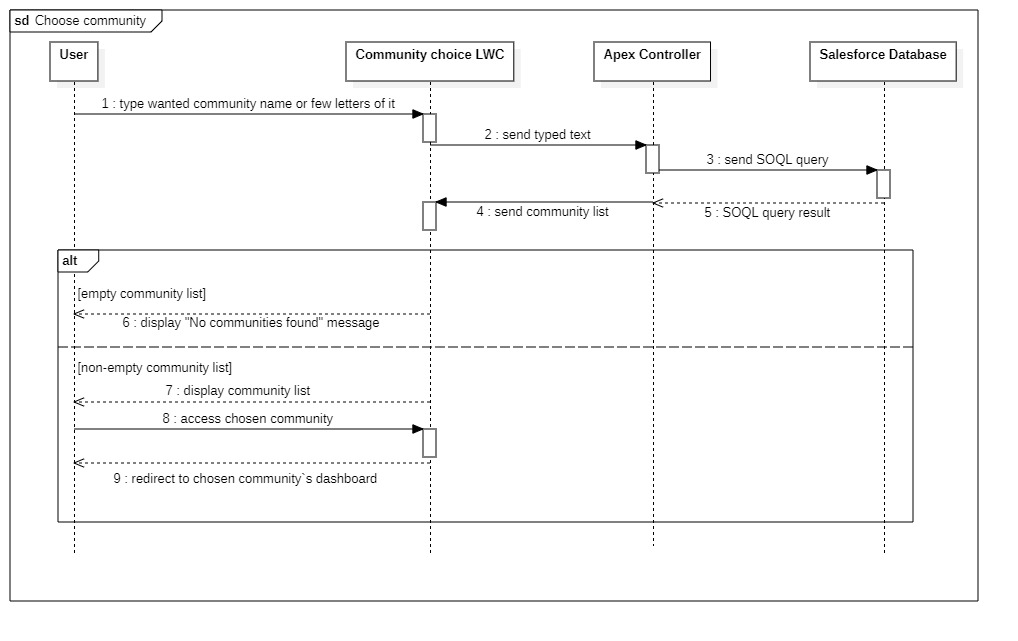
\includegraphics[scale=0.5]{Choose community_seq.jpg}
    \caption{Detailed sequence diagram of the "Choose community" use case}
\end{figure}
\subsection{Detailed sequence diagram of the "Access synthetic dashboard" use case}
The following figure illustrates the detailed sequence diagram of the use case
"Access synthetic dashboard".
This use case starts with opening a dashboard interface specific to the community chosen
by the user. The user may consult the account distribution chart, licenses distribution chart, login attempts distribution chart, time spent in community chart, and developers' error metrics chart where he will be able to select a specific user to monitor their error logs.
  \begin{figure}[H]%
    \center   
    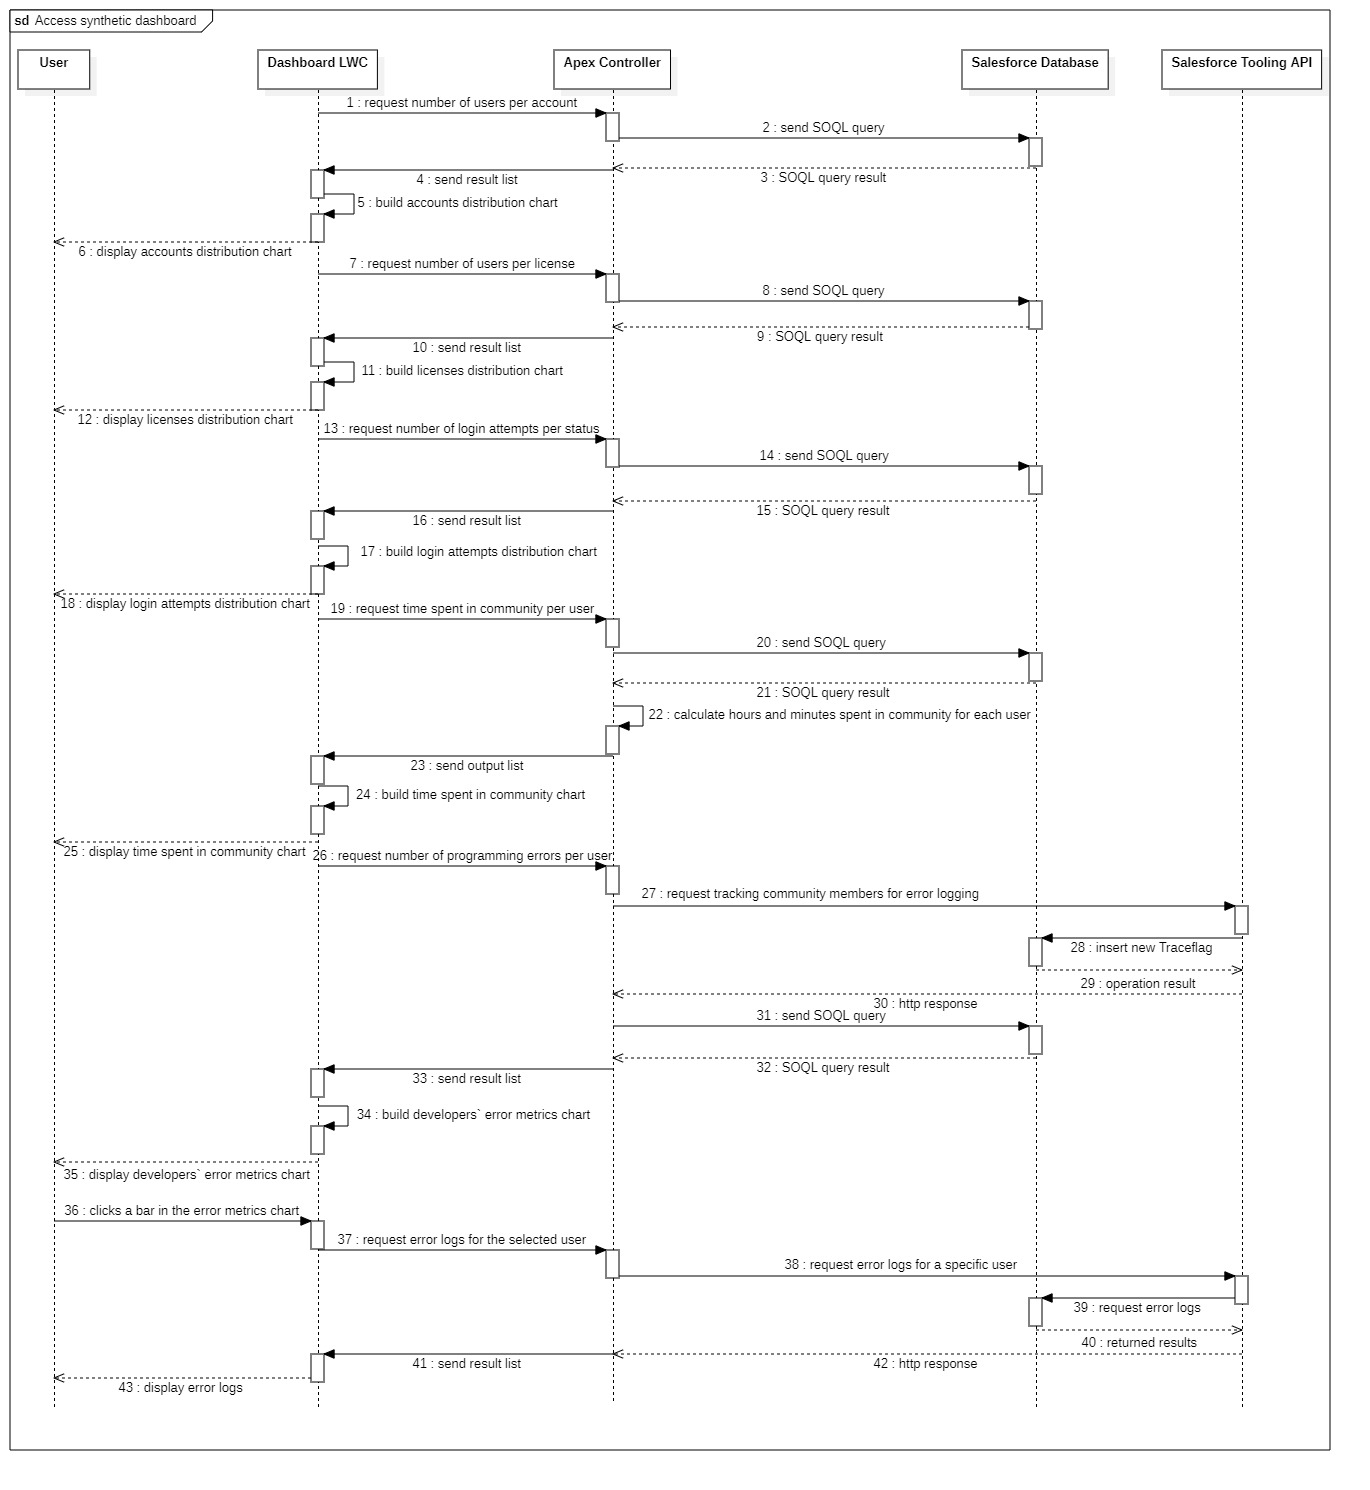
\includegraphics[scale=0.38]{Access synthetic dashboard_seq.jpg}
    \caption{Detailed sequence diagram of the "Access synthetic dashboard" use case}
\end{figure}

\subsection{Detailed sequence diagram of the "Consult users List" use case}
The following figure illustrates the detailed sequence diagram of the use case
"Consult users List".
This use case starts with opening an interface displaying a data table containing information about the user's community members. Then the user may search for a specific user using his Salesforce user name, full name, or his email address, he may also filter given results by account name, user status (active or not active), profile name, or account name. For the displayed members the user may choose to send welcome emails, send reset password emails to selected members as well as update their current status and their information.
 \begin{figure}[H]%
    \center   
    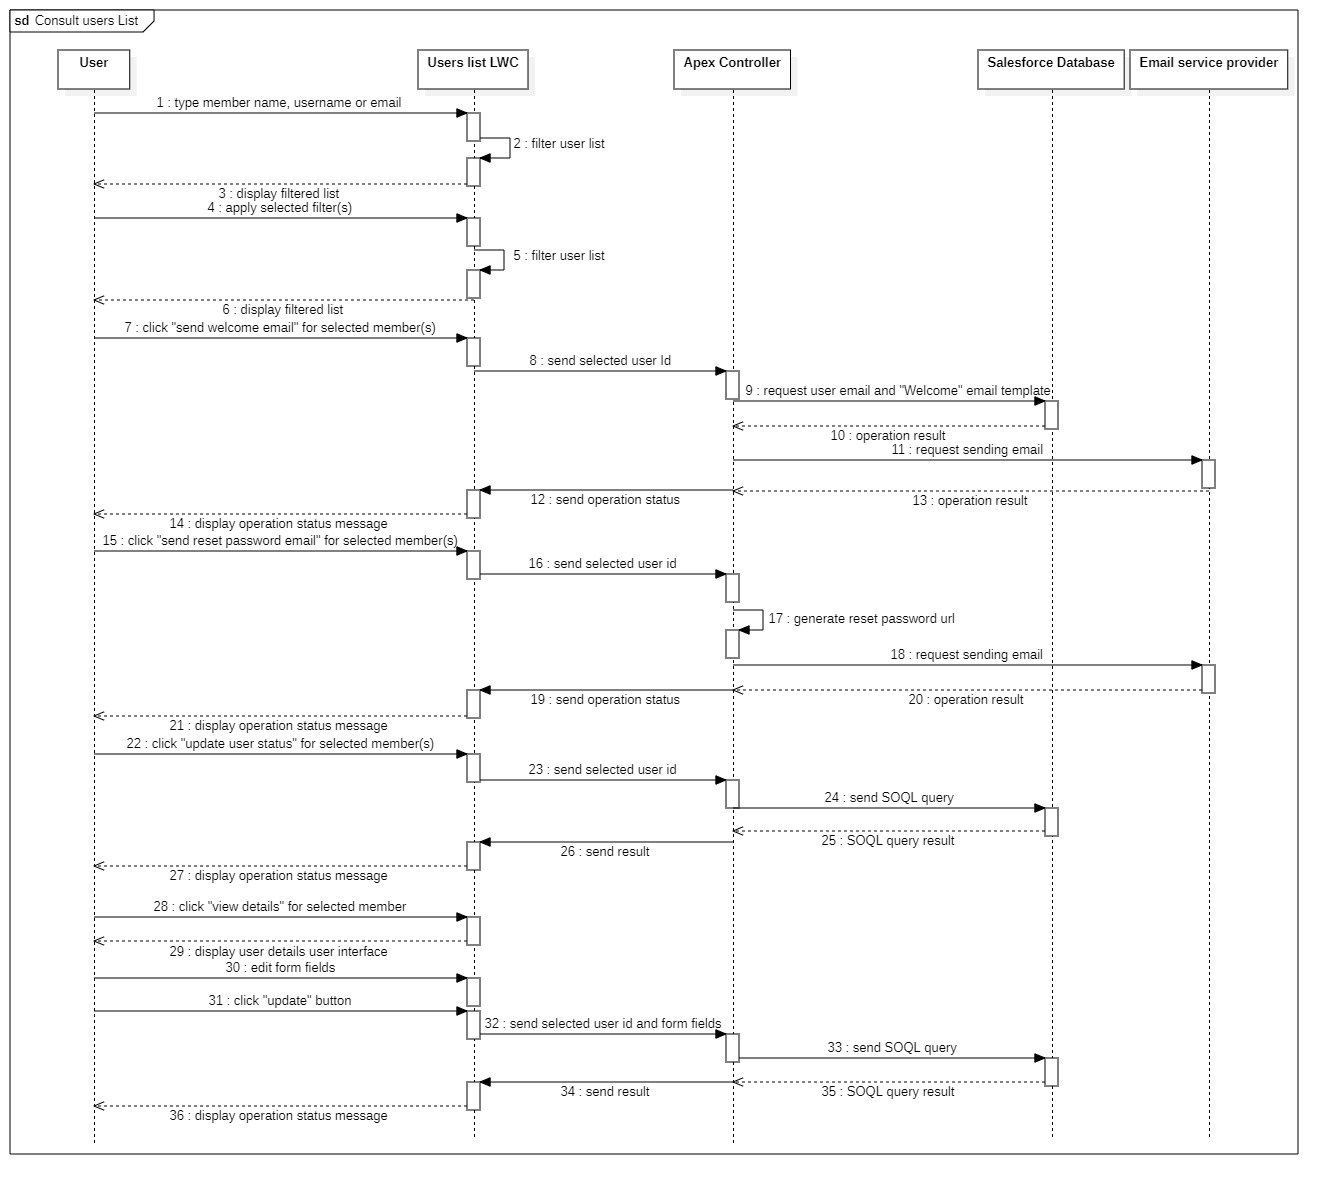
\includegraphics[scale=0.38]{Consult users List_seq.jpg}
    \caption{Detailed sequence diagram of the "Consult users List" use case}
\end{figure}
\subsection{Detailed sequence diagram of the "Add members" use case}
The following figure illustrates the detailed sequence diagram of the use case
"Add members".
This use case starts with opening an interface displaying an empty form containing input fields representing required and optional information about the new community member, the user may choose to add another empty form, add another form containing the same values as the previous one or delete the last form. Afterward, the user may choose to submit all forms where the system will prompt an error message in case one or more required fields are missing, the type user name already exists or the license limits are exceeded, otherwise, the system will prompt the success of the insert operation and will refresh the users' list. 
 \begin{figure}[H]%
    \center   
    \includegraphics[scale=0.4]{Add members_seq.jpg}
    \caption{Detailed sequence diagram of the "Add members" use case}
\end{figure}

\subsection{Detailed sequence diagram of the "Consult failed login attempts" use case}
The following figure illustrates the detailed sequence diagram of the use case
"Consult failed login attempts".
This use case starts with opening an interface displaying a data table containing information about the failed login attempts committed by the user's community members. Then the user may search for a specific login event using the member's Salesforce user name or his full name, he may also filter given results by login event status (invalid password, no community access, etc) or by its date and time. For the displayed events the user may choose to send welcome security warning email to the concerned member or consult details about the full login event.
\begin{figure}[H]%
    \center   
    \includegraphics[scale=0.4]{Consult failed login attempts_seq.jpg}
    \caption{Detailed sequence diagram of the "Consult failed login attempts" use case}
\end{figure}
\subsection{Detailed sequence diagram of the "Consult connection history" use case}
The following figure illustrates the detailed sequence diagram of the use case
"Consult connection history".
This use case starts with opening an interface containing a bar chart displaying the number of logins for each member, the user may filter displayed results by date and time or by time range (yesterday, last week, or last month). For the displayed results the user may select a specific member to access further information about him where he will also be able to update his Salesforce user license.
\begin{figure}[H]%
    \center   
    \includegraphics[scale=0.45]{Consult connection history_seq.jpg}
    \caption{Detailed sequence diagram of the "Consult connection history" use case}
\end{figure}
\subsection{Detailed sequence diagram of the "Access Chatbot" use case}
The following figure illustrates the detailed sequence diagram of the use case
"Access Chatbot".
This use case starts with opening a chat interface where the user may type any question that he wants to ask the digital assistant, he may also select one of the predefined questions proposed by the system, then the system will prompt the answer given by the Chatbot or display an error in case there is one. Next, the user will be asked for feedback regarding the given answer and he will be able to click the like or the dislike button, the given feedback will be saved in the current Salesforce organization database and will be exploited for future updates of the Chatbot.
\begin{figure}[H]%
    \center   
    \includegraphics[scale=0.5]{Access Chatbot_seq.jpg}
    \caption{Detailed sequence diagram of the "Access Chatbot" use case}
\end{figure}
\section*{Conclusion}
This chapter presents one of the most important phases of the process of
development of a project: conception subdivided into the overall conception
and detailed conception.\\
We presented an MVC pattern and we
explained its application in our case. We have described the dynamic view
of the system through a set of sequence diagrams.\\
The following chapter will deal with the implementation of the project illustrated by screenshots of different interfaces. We will describe the environment of
work and the tools used too.
    % \cleardoublepage%

    % Back matter
    % @Author: Jacem Chaieb
% @Date:   2015-07-26 13:42:06
% @Last Modified by:   Jacem Chaieb
% @Last Modified time: 2016-04-12 15:45:56

\chapter*{Conclusion and perspectives }
\addcontentsline{toc}{chapter}{Conclusion and perspectives}

\markboth{\MakeUppercase{Conclusion and perspectives}}{}%
Admittedly, the diversity of lightning applications is an enrichment
world of Salesforce extensions, where everything goes through these applications
to facilitate tasks, bring more comfort, and gain in
time and money.\\
The objective of this report is to present the application carried out
during our end of studies internship project within the company TechLead. Our application facilitates the task of managing the members of Salesforce communities for community managers and administrators. The app
carried out also integrates a smart Salesforce digital assistant and a synthetic dashboard for community directors.\\
This internship allowed us to improve our technical Salesforce knowledge given
that we used a variety of technologies associated with said platform.
On the other hand, during this
internship, we got used to professional life and teamwork as well as time management regarding software development.
To conclude, our realized application can be extended by further improving the Chatbot feature, as well as adding an event notification system.
It is also possible to make our application multilingual in future updates.
    \cleardoublepage%

   

    % @Author: Jacem Chaieb
% @Date:   2015-07-26 13:42:06
% @Last Modified by:   Jacem Chaieb
% @Last Modified time: 2016-04-12 15:35:09

%%%%%%%%%%%%%%%%%%%%%%%%%%%%%%%%%%%%%%%%%%%%%%%%%%%%
% Don't touch this, it is auto generated
%%%%%%%%%%%%%%%%%%%%%%%%%%%%%%%%%%%%%%%%%%%%%%%%%%%%
\nocite{*}

\phantomsection{}
\addcontentsline{toc}{chapter}{Webography}
\printbibliography[title={Webography},type=online]

\phantomsection{}
\addcontentsline{toc}{chapter}{Bibliography}
\printbibliography[title={Bibliography},nottype=online]

    \cleardoublepage%

    

    \addtocontents{toc}{\protect\setcounter{tocdepth}{3}}

  \end{pfe-enis}
  
  \begin{thebibliography}{9}
\bibitem{1}
Get Started with the Salesforce Platform.
[\href{https://trailhead.salesforce.com/content/learn/modules/starting_force_com/starting_intro}{trailhead.salesforce.com}].
\bibitem{2}
Discover Use Cases for the Platform.
[\href{https://trailhead.salesforce.com/content/learn/modules/starting_force_com/starting_discovering}{trailhead.salesforce.com}].
\bibitem{3}
Understand the Salesforce Architecture.
[\href{https://trailhead.salesforce.com/content/learn/modules/starting_force_com/starting_understanding_arch}{trailhead.salesforce.com}].
\bibitem{4}
Oumayma LAZREG : Rapport PFE, Conception et développement
d'une application mobile
intelligente de e \_ consulation et
d'estimation des maladies.
(ISSAT de Sousse), 2019.
\bibitem{5}
Model-View-Controller design pattern.
[\href{https://help.hcltechsw.com/commerce/9.1.0/developer/concepts/csdmvcdespat.html}{help.hcltechsw.com}].
\bibitem{6}
Model–view–controller
[\href{https://en.wikipedia.org/wiki/Model-view-controller}{en.wikipedia.org}].
\bibitem{7}
What is MVC Design Pattern?
[\href{https://www.educba.com/what-is-mvc-design-pattern/}{www.educba.com}].
\bibitem{8}
What is Apex?
[\href{https://developer.salesforce.com/docs/atlas.en-us.apexcode.meta/apexcode/apex_intro_what_is_apex.htm}{developer.salesforce.com}].
\bibitem{9}
Lightning Aura Components Developer Guide
[\href{https://developer.salesforce.com/docs/atlas.en-us.lightning.meta/lightning/intro_components.htm}{developer.salesforce.com}].





\end{thebibliography}
\end{document}